\documentclass[12pt]{book}
%\usepackage{pdf14}
%Paper saving
%\documentclass[12pt,openany]{book}
%\documentclass[10pt,openany]{book}
%\documentclass[8pt,openany]{extbook}

\usepackage[T1]{fontenc}

% Footnotes should use symbols, not numbers.  Numbered footnotes are
% evil
\usepackage[perpage,symbol*]{footmisc}

%\usepackage{enumerate}
\usepackage[shortlabels]{enumitem}
\usepackage{ifpdf}
\usepackage{amsmath}
\usepackage{amsfonts}
\usepackage{amssymb}
\usepackage{amsthm}
\usepackage[pdftex]{graphicx}
%\usepackage{color}
%\usepackage{graphics}
\usepackage[headings]{fullpage}
%\usepackage{url}
\usepackage{varioref}
%\usepackage{floatflt}
%\usepackage{wrapfig}
\usepackage{makeidx}
\usepackage[pdftex]{hyperref}
\usepackage[all]{hypcap}
\usepackage[shortalphabetic]{amsrefs}
\usepackage[all]{xy}
\usepackage{nicefrac}
\usepackage{microtype}

\usepackage{tikz}
\usepackage{rotating}



% Times
%\usepackage{txfonts}
% Times, but symbol/cm/ams math fonts
\usepackage{mathptmx}
% But we do want helvetica for sans
\usepackage{helvet}

%enumitem global options
\setlist{leftmargin=*,itemsep=0.5\itemsep,parsep=0.5\parsep,topsep=0.5\topsep,partopsep=0.5\partopsep}


% useful
\newcommand{\ignore}[1]{}

% analysis/geometry stuff
\newcommand{\ann}{\operatorname{ann}}
\renewcommand{\Re}{\operatorname{Re}}
\renewcommand{\Im}{\operatorname{Im}}
\newcommand{\Orb}{\operatorname{Orb}}
\newcommand{\hol}{\operatorname{hol}}
\newcommand{\aut}{\operatorname{aut}}
\newcommand{\codim}{\operatorname{codim}}
\newcommand{\sing}{\operatorname{sing}}

% reals
\newcommand{\esssup}{\operatorname{ess~sup}}
\newcommand{\essran}{\operatorname{essran}}
\newcommand{\innprod}[2]{\langle #1 | #2 \rangle}
\newcommand{\linnprod}[2]{\langle #1 , #2 \rangle}
\newcommand{\supp}{\operatorname{supp}}
\newcommand{\Nul}{\operatorname{Nul}}
\newcommand{\Ran}{\operatorname{Ran}}
\newcommand{\sabs}[1]{\lvert {#1} \rvert}
\newcommand{\snorm}[1]{\lVert {#1} \rVert}
\newcommand{\abs}[1]{\left\lvert {#1} \right\rvert}
\newcommand{\norm}[1]{\left\lVert {#1} \right\rVert}

% sets (some)
\newcommand{\C}{{\mathbb{C}}}
\newcommand{\R}{{\mathbb{R}}}
\newcommand{\Z}{{\mathbb{Z}}}
\newcommand{\N}{{\mathbb{N}}}
\newcommand{\Q}{{\mathbb{Q}}}
\newcommand{\D}{{\mathbb{D}}}
\newcommand{\F}{{\mathbb{F}}}

% consistent
\newcommand{\bB}{{\mathbb{B}}}
\newcommand{\bC}{{\mathbb{C}}}
\newcommand{\bR}{{\mathbb{R}}}
\newcommand{\bZ}{{\mathbb{Z}}}
\newcommand{\bN}{{\mathbb{N}}}
\newcommand{\bQ}{{\mathbb{Q}}}
\newcommand{\bD}{{\mathbb{D}}}
\newcommand{\bF}{{\mathbb{F}}}
\newcommand{\bH}{{\mathbb{H}}}
\newcommand{\bO}{{\mathbb{O}}}
\newcommand{\bP}{{\mathbb{P}}}
\newcommand{\bK}{{\mathbb{K}}}
\newcommand{\bV}{{\mathbb{V}}}
\newcommand{\CP}{{\mathbb{CP}}}
\newcommand{\RP}{{\mathbb{RP}}}
\newcommand{\HP}{{\mathbb{HP}}}
\newcommand{\OP}{{\mathbb{OP}}}
\newcommand{\sA}{{\mathcal{A}}}
\newcommand{\sB}{{\mathcal{B}}}
\newcommand{\sC}{{\mathcal{C}}}
\newcommand{\sF}{{\mathcal{F}}}
\newcommand{\sG}{{\mathcal{G}}}
\newcommand{\sH}{{\mathcal{H}}}
\newcommand{\sM}{{\mathcal{M}}}
\newcommand{\sO}{{\mathcal{O}}}
\newcommand{\sP}{{\mathcal{P}}}
\newcommand{\sQ}{{\mathcal{Q}}}
\newcommand{\sR}{{\mathcal{R}}}
\newcommand{\sS}{{\mathcal{S}}}
\newcommand{\sI}{{\mathcal{I}}}
\newcommand{\sL}{{\mathcal{L}}}
\newcommand{\sK}{{\mathcal{K}}}
\newcommand{\sU}{{\mathcal{U}}}
\newcommand{\sV}{{\mathcal{V}}}
\newcommand{\sX}{{\mathcal{X}}}
\newcommand{\sY}{{\mathcal{Y}}}
\newcommand{\sZ}{{\mathcal{Z}}}
\newcommand{\fS}{{\mathfrak{S}}}

\newcommand{\interior}{\operatorname{int}}

% Topo stuff
\newcommand{\id}{\textit{id}}
\newcommand{\im}{\operatorname{im}}
\newcommand{\rank}{\operatorname{rank}}
\newcommand{\Tor}{\operatorname{Tor}}
\newcommand{\Torsion}{\operatorname{Torsion}}
\newcommand{\Ext}{\operatorname{Ext}}
\newcommand{\Hom}{\operatorname{Hom}}

%extra thingies
\newcommand{\mapsfrom}{\ensuremath{\text{\reflectbox{$\mapsto$}}}}
\newcommand{\from}{\ensuremath{\leftarrow}}
\newcommand{\dhat}[1]{\hat{\hat{#1}}}
\newcommand{\spn}{\operatorname{span}}

% San Serif fonts
%\renewcommand{\familydefault}{\sfdefault}

% To allow skrinking to 5.5 x 8.5 inches without whitespaces
% Make sure to rerun makeindex as well
% Useful for printing on lilu.com and saving on paper
%\addtolength{\textheight}{2.13in}
%\addtolength{\paperheight}{2.13in}

% unfortunatley colorlinks prints, and ocgcolorlinks doesn't split links
% or typeset all links well, etc..
\hypersetup{
    %colorlinks,
    pdfborderstyle={/S/U/W 0.5},
    %citecolor=black,
    %filecolor=black,
    %linkcolor=black,
    %urlcolor=black,
    pdfkeywords={real analysis, Riemann integral, derivative, limit, sequence},
    pdfsubject={Real Analysis},
    pdftitle={Basic Analysis III: Introduction to Real Analysis, Volume III},
    pdfauthor={Jiri Lebl}
}

% Set up our index
\makeindex

% Very simple indexing
\newcommand{\myindex}[1]{#1\index{#1}}

% define this to be empty to kill notes
\newcommand{\sectionnotes}[1]{\noindent \emph{Note: #1} \medskip \par}

% Define this to be empty to not skip page before the sections to
% save some paper
\newcommand{\sectionnewpage}{\clearpage}
%\newcommand{\sectionnewpage}{}

\author{Ji\v{r}\'i Lebl}

\title{Basic Analysis III: Introduction to Real Analysis, Volume III}

% Don't include subsections
\setcounter{tocdepth}{1}

\theoremstyle{plain}
\newtheorem{thm}{Theorem}[section]
\newtheorem{lemma}[thm]{Lemma}
\newtheorem{prop}[thm]{Proposition}
\newtheorem{cor}[thm]{Corollary}

\theoremstyle{remark}
\newtheorem{remark}[thm]{Remark}

\theoremstyle{definition}
\newtheorem{defn}[thm]{Definition}

\newtheoremstyle{exercise}% name
  {}% Space above
  {}% Space below
  {\itshape \small}% Body font
  {}% Indent amount 1
  {\bfseries \itshape \small}% Theorem head font
  {:}% Punctuation after theorem head
  {.5em}% Space after theorem head 2
  {}% Theorem head spec (can be left empty, meaning "normal")

\newenvironment{exnote}{\small}{}

\theoremstyle{exercise}
\newtheorem{exercise}{Exercise}[section]

\newtheoremstyle{example}% name
  {}% Space above
  {}% Space below
  {}% Body font
  {}% Indent amount 1
  {\bfseries}% Theorem head font
  {:}% Punctuation after theorem head
  {.5em}% Space after theorem head 2
  {}% Theorem head spec (can be left empty, meaning "normal")

\theoremstyle{example}
\newtheorem{example}[thm]{Example}

% referencing
\newcommand{\figureref}[1]{\hyperref[#1]{Figure~\ref*{#1}}}
\newcommand{\tableref}[1]{\hyperref[#1]{Table~\ref*{#1}}}
\newcommand{\chapterref}[1]{\hyperref[#1]{chapter~\ref*{#1}}}
\newcommand{\Chapterref}[1]{\hyperref[#1]{Chapter~\ref*{#1}}}
\newcommand{\sectionref}[1]{\hyperref[#1]{\S\ref*{#1}}}
\newcommand{\exerciseref}[1]{\hyperref[#1]{Exercise~\ref*{#1}}}
\newcommand{\exampleref}[1]{\hyperref[#1]{Example~\ref*{#1}}}
\newcommand{\thmref}[1]{\hyperref[#1]{Theorem~\ref*{#1}}}
\newcommand{\propref}[1]{\hyperref[#1]{Proposition~\ref*{#1}}}
\newcommand{\lemmaref}[1]{\hyperref[#1]{Lemma~\ref*{#1}}}
\newcommand{\corref}[1]{\hyperref[#1]{Corollary~\ref*{#1}}}
\newcommand{\defnref}[1]{\hyperref[#1]{Definition~\ref*{#1}}}

\begin{document}

\setcounter{chapter}{0}
\refstepcounter{chapter}
\label{rn:chapter}
\refstepcounter{chapter}
\label{seq:chapter}
\refstepcounter{chapter}
\label{lim:chapter}
\refstepcounter{chapter}
\label{der:chapter}
\refstepcounter{chapter}
\label{int:chapter}
\refstepcounter{chapter}
\label{fs:chapter}
\refstepcounter{chapter}
\label{ms:chapter}

\refstepcounter{chapter}
\refstepcounter{chapter}
\refstepcounter{chapter}

%\let\oldchapter\chapter
%\renewcommand*{\chapter}[1]{\oldchapter[#1]{#1 \hspace{\fill} {\rm \normalsize \today}}}

\ifpdf
  \pdfbookmark{Title Page}{title}
\fi
\newlength{\centeroffset}
\setlength{\centeroffset}{-0.5\oddsidemargin}
\addtolength{\centeroffset}{0.5\evensidemargin}
%\addtolength{\textwidth}{-\centeroffset}
\thispagestyle{empty}
\vspace*{\stretch{1}}
\noindent\hspace*{\centeroffset}\makebox[0pt][l]{\begin{minipage}{\textwidth}
\flushright
{\Huge\bfseries \sffamily Basic Analysis III }
\noindent\rule[-1ex]{\textwidth}{5pt}\\[2.5ex]
\hfill\emph{\Large \sffamily Introduction to Real Analysis, Volume III}
\end{minipage}}

\vspace{\stretch{1}}
\noindent\hspace*{\centeroffset}\makebox[0pt][l]{\begin{minipage}{\textwidth}
\flushright
{\bfseries 
by Ji{\v r}\'i Lebl\\[3ex]} 
\today
\end{minipage}}

%\addtolength{\textwidth}{\centeroffset}
\vspace{\stretch{2}}


\pagebreak

\vspace*{\fill}

%\begin{small} 
\noindent
Typeset in \LaTeX.

\bigskip

\noindent
Copyright \copyright 2012--2016 Ji{\v r}\'i Lebl

\bigskip

%\begin{floatingfigure}{1.4in}
%\vspace{-0.05in}
\noindent

\includegraphics[width=1.38in]{license}
%\end{floatingfigure}

\bigskip

\noindent
This work is licensed under the Creative Commons
Attribution-Non\-commercial-Share Alike 3.0 United States License. To view a
copy of this license, visit
\url{http://creativecommons.org/licenses/by-nc-sa/3.0/us/} or send a letter to
Creative Commons, 171 Second Street, Suite 300, San Francisco, California,
94105, USA.
%\end{small}

\bigskip

\noindent
You can use, print, duplicate, share these notes as much as you want.  You can
base your own notes on these and reuse parts if you keep the license the
same.  If you plan to use these commercially (sell them for more than just
duplicating cost), then you need to contact me and we will work something out.
If you are printing a course pack for your students, then it is fine if the 
duplication service is charging a fee for printing and selling the printed
copy.  I consider that duplicating cost.

\bigskip

\noindent
During the writing of these notes, 
the author was in part supported by NSF grant DMS-1362337.

\bigskip

\noindent
See \url{http://www.jirka.org/ra2/} for more information
(including contact information).


% For large print do this
%\large

\microtypesetup{protrusion=false}
\tableofcontents
\microtypesetup{protrusion=true}

\newpage

%%%%%%%%%%%%%%%%%%%%%%%%%%%%%%%%%%%%%%%%%%%%%%%%%%%%%%%%%%%%%%%%%%%%%%%%%%%%%%
%%%%%%%%%%%%%%%%%%%%%%%%%%%%%%%%%%%%%%%%%%%%%%%%%%%%%%%%%%%%%%%%%%%%%%%%%%%%%%
%%%%%%%%%%%%%%%%%%%%%%%%%%%%%%%%%%%%%%%%%%%%%%%%%%%%%%%%%%%%%%%%%%%%%%%%%%%%%%

\chapter*{Introduction}
\addcontentsline{toc}{chapter}{Introduction}
\markboth{INTRODUCTION}{INTRODUCTION}

%%%%%%%%%%%%%%%%%%%%%%%%%%%%%%%%%%%%%%%%%%%%%%%%%%%%%%%%%%%%%%%%%%%%%%%%%%%%%%

\section*{About this book}

This book is the continuation of ``Basic Analysis''.  The book is meant to
be a seamless continuation, so the chapters are numbered to start where the
first volume left off.

This book is unfinished, and at this point is likely in a state of
constant flux, and will have possibly more topics added on the end (or even
in the middle).
Numbering will
change, things will get reshuffled.  Do not expect constancy, that is,
at least for now.  At
some point in the future, this book will also become stable, but until then,
you have been warned.

%%%%%%%%%%%%%%%%%%%%%%%%%%%%%%%%%%%%%%%%%%%%%%%%%%%%%%%%%%%%%%%%%%%%%%%%%%%%%%


%%%%%%%%%%%%%%%%%%%%%%%%%%%%%%%%%%%%%%%%%%%%%%%%%%%%%%%%%%%%%%%%%%%%%%%%%%%%%%
%%%%%%%%%%%%%%%%%%%%%%%%%%%%%%%%%%%%%%%%%%%%%%%%%%%%%%%%%%%%%%%%%%%%%%%%%%%%%%
%%%%%%%%%%%%%%%%%%%%%%%%%%%%%%%%%%%%%%%%%%%%%%%%%%%%%%%%%%%%%%%%%%%%%%%%%%%%%%

\chapter{Sequences and series of functions} \label{seqser:chapter}

%%%%%%%%%%%%%%%%%%%%%%%%%%%%%%%%%%%%%%%%%%%%%%%%%%%%%%%%%%%%%%%%%%%%%%%%%%%%%%

\section{Complex numbers}
\label{sec:complexnums}

\sectionnotes{FIXME4 lectures}

A complex number is just a pair $(x,y) \in \R^2$ on which we define
multiplication below.
We call the set of complex numbers $\C$.
We identify $x \in \R$ with $(x,0) \in \C$.
The $x$-axis is then called the \emph{real axis} and the $y$-axis is
called the \emph{imaginary axis}.  The set $\C$ is sometimes called the
\emph{complex plane}.

%\bnote{DRAW complex plane}
%\textbf{FIXME: DRAW complex plane}

Define
\begin{align*}
& (x,y) + (s,t) := (x+s,y+t) \\
& (x,y) (s,t) := (xs-yt,xt+ys)
\end{align*}
Under the identification above we have $0 = (0,0)$ and $1 = (1,0)$.  These
properties then give a field.

\begin{exercise}
Check that these give a field.
\end{exercise}

Generally, we write complex number $(x,y)$ as $x+iy$, where we
define\footnote{Note that engineers use $j$ instead of $i$.}
\begin{equation*}
i := (0,1) .
\end{equation*}
Notice that $i^2 = (0,1)(0,1) = (0-1,0+0) = -1$.
So we have a solution to the polynomial equation
\begin{equation*}
z^2+1=0 .
\end{equation*}
From now on, we will not use the notation $(x,y)$ and use only $x+iy$.

We generally use $x,y,r,s,t$ for real values and $z,w,\xi,\zeta$
for complex values, although that is not a hard and fast rule.  In
particular $z$ is often just used as a third real variable in $\R^3$.

\begin{defn}
Let $z= x+iy$.
Define
the \emph{\myindex{real part}} of $z$ as $x$, and the
the \emph{\myindex{imaginary part}} of $z$ as $y$.  We write
\begin{align*}
& \Re z := x , \\
& \Im z := y .
\end{align*}
Define the
\emph{\myindex{complex conjugate}} as
\begin{equation*}
\bar{z} := x-iy .
\end{equation*}
Similarly define \emph{\myindex{modulus}} as
\begin{equation*}
\abs{z} := \sqrt{x^2+y^2} .
\end{equation*}
\end{defn}

Think of the complex conjugate as a reflection across the real axis.
We note that the real numbers are precisely those for which the imaginary
part $y=0$.  In particular they are precisely those numbers which satisfy
the equation
\begin{equation*}
z = \bar{z} .
\end{equation*}
That is, real numbers are precisely those numbers fixed by the reflection.

As $\C$ is really $\R^2$, we let the metric on $\C$ be the standard
euclidean metric on $\R^2$.
In particular,
\begin{equation*}
\abs{z} = d(z,0) , \qquad 
\text{and also} \qquad 
\abs{z-w} = d(z,w) .
\end{equation*}
We therefore think of $\abs{z-w}$ as our metric, and the topology on $\C$ is
the same topology we get on $\R^2$ with the euclidean metric.
We therefore immediately get

\begin{prop}[Triangle inequality]
\begin{align*}
\abs{z+w} & \leq \abs{z}+\abs{w} \\
\big\lvert \abs{z}-\abs{w} \big\rvert & \leq \abs{z-w}
\end{align*}
\end{prop}

The complex conjugate and the modulus are even more intimately related:
\begin{equation*}
\abs{z}^2 =
x^2+y^2 =
(x+iy)(x-iy) =
z \bar{z} .
\end{equation*}

\begin{remark}
It is good to notice that there is no natural ordering on the complex numbers.
Definitely no ordering that makes the complex numbers into an ordered field.
Ordering is one of the major things we lose when we go from real to complex
numbers.
\end{remark}


Most things that we proved about real numbers that did not require
the ordering carries over.  Also, the standard topology on $\C$ is
just the standard topology on $\R^2$, using the modulus for our distance
as above.  Hence we can carry over all that we know about the metric
space $\R^2$ to $\C$.  In particular we know what limits of
sequences mean, we know about complex-valued functions and their continuity,
we know that $\C$ is a \textbf{complete metric space},
etc...

It is also not hard to show that the algebraic operations are
continuous.  This is because convergence in 
$\R^2$ is the same as convergence for each component.  So for example:
let $z_n = x_n + iy_n$ and
$w_n = s_n + it_n$ and suppose that
$\lim z_n = z = x+iy$ and $\lim w_n = w = s+it$.
Let us show that
$$
\lim_{n\to\infty} z_n w_n = zw
$$
Note that as topology on $\C$ is the same as on $\R^2$, then
$x_n \to x$, $y_n \to y$, $s_n \to s$, and $t_n \to t$.  Then
$$
z_n w_n = (x_ns_n-y_nt_n) + i(x_nt_n+y_ns_n)
$$
now 
$\lim (x_ns_n-y_nt_n) = xs-yt$ and
$\lim (x_nt_n+y_ns_n) = xt+ys$ and
$(xs-yt)+i(xt+ys) = zw$ so
$$
\lim_{n\to\infty} z_n w_n = zw
$$
The rest is left to student.  

Similarly the modulus, and complex conjugate are continuous functions.

FIXME: the above should be a proposition.

It is often useful to extend the definition of the exponential to complex
numbers.  We define the \emph{\myindex{complex exponential}} as
\begin{equation*}
e^{x+iy} := e^x \bigl( \cos(y) + i \sin(y) \bigr) .
\end{equation*}
It should be noted that at this point we assume that cosine and sine
have been somehow defined.  We will get to rigorously
construct cosine and sine later using power series.  In fact,
the way we will define cosine and sine is to define 
$e^{x+iy}$ for all complex numbers using power series and then simply
extract cosine and sine out of it.

With this notation you can write complex number in polar coordinates
as
\begin{equation*}
x+iy = r e^{i\theta} .
\end{equation*}
Here, $r \geq 0$ is the modulus of $x+iy$ and $\theta$ is what is called
the \emph{\myindex{argument}}.

FIXME

FIXME: convergence of series

FIXME: integration of complex valued functions


%%%%%%%%%%%%%%%%%%%%%%%%%%%%%%%%%%%%%%%%%%%%%%%%%%%%%%%%%%%%%%%%%%%%%%%%%%%%%%

\sectionnewpage
\section{Continuity of limits}
\label{sec:FIXME}

\sectionnotes{FIXME4 lectures}

Let us get back to swapping on limits.  Let $\{ f_n \}$ be a sequence
of functions $f_n \colon X \to Y$ for a set $X$ and a metric space $Y$.
Let $f \colon X \to Y$ be a
function and for every $x \in X$ suppose that
\begin{equation*}
f(x) = \lim_{n\to \infty} f_n(x) .
\end{equation*}
We say the sequence $\{ f_n \}$ \emph{converges pointwise} to
$f$.

Question is:
If $f_n$ are all continuous, is $f$ continuous?  Differentiable?
Integrable?  What are the derivatives or integrals of $f$?

For example for continuity of the pointwise limitwe are asking if
\begin{equation}
\lim_{x\to x_0} \lim_{n\to\infty} f_n(x)
\overset{?}{=}
\lim_{n\to\infty} \lim_{x\to x_0} f_n(x)
\end{equation}
We don't even know a priory if both sides exist, let alone equal each other.

\begin{example}
The functions $f_n \colon \R \to \R$,
\begin{equation*}
f_n(x) := \frac{1}{1+nx^2}
\end{equation*}
converge pointwise to
\begin{equation*}
f(x) = 
\begin{cases}
1 & \text{ if $x=0$} \\
0 & \text{ else}
\end{cases}
\end{equation*}
which is not continuous of course.
\end{example}

Similarly if $Y=\C$, we can have a pointwise convergence of a series,
for every $x \in X$ we can have
\begin{equation*}
f(x) = \lim_{n\to \infty} \sum_{k=1}^n f_k(x) =
\sum_{k=1}^\infty f_k(x) .
\end{equation*}

We saw continuity is preserved if we require a stronger convergence,
that is, we require uniform convergence.

Let $f_n \colon X \to Y$ be functions.  Then
$\{f_n\}$ \emph{converges uniformly} to $f$ if
for every $\epsilon > 0$, there exists an $M$ such that
for all $n \geq M$ and all $x \in X$ we have
\begin{equation*}
d\bigl(f_n(x),f(x)\bigr) < \epsilon
\end{equation*}
If we are dealing with complex-valued functions then
\begin{equation*}
\abs{f_n(x)-f(x)} < \epsilon .
\end{equation*}

Similarly a series of functions converges uniformly if the sequence of
partial sums converges uniformly, that is for every $\epsilon > 0$
there exists an $M$ such that
for all $n \geq M$ and all $x \in X$ we have
\begin{equation*}
\abs{\left(\sum_{k=1}^nf_k(x)\right)-f(x)} < \epsilon .
\end{equation*}

Again recall from chapter FIXME that this is stronger than pointwise
convergence.  Pointwise convergence can be stated as:
$\{f_n\}$ \emph{\myindex{converges pointwise}} to $f$ if
for every $x \in X$ and
every $\epsilon > 0$, there exists an $M$ such that
for all $n \geq M$ we have
\begin{equation*}
d\bigl(f_n(x),f(x)\bigr) < \epsilon .
\end{equation*}

Note that for uniform convergence $M$ does not depend on $x$.  We need to
have one $M$ that works for all $M$.

\begin{thm}
%\medskip
%\textbf{Theorem 7.8:}
Let $f_n \colon X \to \C$ be functions.  Then $\{ f_n \}$ converges
uniformly if and only if for every $\epsilon > 0$, there is an $M$ such that
for all $n, m \geq M$, and all $x \in X$ we have
\begin{equation*}
\abs{f_n(x)-f_m(x)} < \epsilon .
\end{equation*}
\end{thm}

\begin{proof}
Suppose that $\{f_n\}$ converges uniformly to some $f \colon X \to \C$.  Then 
find $M$ such that for all $n \geq M$ we have
\begin{equation*}
\abs{f_n(x)-f(x)} < \frac{\epsilon}{2} \qquad \text{for all $x \in X$.}
\end{equation*}
Then for all $m,n \geq M$ we have
\begin{equation*}
\abs{f_n(x)-f_m(x)}
\leq
\abs{f_n(x)-f(x)} + \abs{f(x)-f_m(x)} < \frac{\epsilon}{2} + \frac{\epsilon}{2}
= \epsilon .
\end{equation*}

For the other direction, first fix $x$.
The sequence
of complex numbers $\{ f_n(x) \}$ is Cauchy and so has a limit
$f(x)$.

Given $\epsilon > 0$ find an $M$ such that
for all $n, m \geq M$, and all $x \in X$ we have
\begin{equation*}
\abs{f_n(x)-f_m(x)} < \epsilon
\end{equation*}
We know that $\lim f_m(x) = f(x)$, so
as compositions of continuous functions are continuous
and algebraic operations and the modulus are continuous we have
\begin{equation*}
\abs{f_n(x)-f(x)} \leq \epsilon .
\end{equation*}
The nonstrict inequality is no trouble.
\end{proof}

Sometimes we write for $f \colon X \to \C$
\begin{equation*}
\snorm{f}_u = \sup_{x \in X} \abs{f(x)} .
\end{equation*}
This is the \emph{\myindex{supremum norm}} or \emph{\myindex{uniform norm}}.
Then we have that
$f_n \colon X \to \C$ converge to $f$ if and only if
\begin{equation*}
\lim_{n\to \infty} \snorm{f_n-f}_u = 0
\end{equation*}
That is if
\begin{equation*}
\lim_{n\to \infty} \left( \sup_{x \in X} \abs{f_n(x)-f(x)} \right) = 0
\end{equation*}

The supermum norm satisfies the triangle inequality:
\begin{equation*}
\abs{f(x)+g(x)} \leq
\abs{f(x)}+\abs{g(x)} \leq
\snorm{f(x)}_u+\snorm{g(x)}_u .
\end{equation*}
Now take a supremum on the left to get
\begin{equation*}
\snorm{f(x)+g(x)}_u \leq
\snorm{f(x)}_u+\snorm{g(x)}_u .
\end{equation*}

For a compact $X$,
the uniform norm is a norm on the vector space $C(X,\C)$.
If $f \colon X \to \C$ is continuous and $X$ is compact then $f$
is bounded and so $\snorm{f}_u < \infty$.
So we can also think of $C(X,\C)$ as a metric space with the
metric $d(f,g) = \snorm{f-g}_u$.
Convergence in the metric space $C(X,\C)$ is
uniform convergence.

\begin{thm}[\myindex{Weierstrass M-test}]
%\medskip
%\textbf{Theorem 7.10} (Weierstrass M-test)
Suppose that $f_n \colon X \to \C$ are functions,
$$
\abs{f_n(x)}\leq M_n
$$
and
$$
\sum_{n=1}^\infty M_n
$$
converges.
Then
$$\sum_{n=1}^\infty f_n(x)$$
converges uniformly.
\end{thm}

Note that the converse of this theorem is not true.

\begin{proof}
Suppose that $\sum M_n$ converges.  Given $\epsilon > 0$,
we have that the partial sums of $\sum M_n$ are Cauchy so for
there is an $N$ such that for all $m, n \geq N$ with $m \geq n$ we have
$$
\sum_{k=n+1}^m M_k < \epsilon
$$
Now let us look at a Cauchy difference of the partial
sums of the functions
$$
\abs{\sum_{k=n+1}^m f_k(x)} \leq
\sum_{k=n+1}^m \abs{f_k(x)} \leq
\sum_{k=n+1}^m M_k < \epsilon .
$$
And we are done by Theorem 7.8.
\end{proof}

\textbf{Examples:}

\begin{example}
The series
\begin{equation*}
\sum_{n=1}^\infty \frac{\sin(nx)}{n^2}
\end{equation*}
converges uniformly on $\R$. (Note: this is a Fourier series,
we will see more of these later).  That is because
\begin{equation*}
\abs{\frac{\sin(nx)}{n^2}} \leq 
\frac{1}{n^2}
\end{equation*}
and
\begin{equation*}
\sum_{n=1}^\infty \frac{1}{n^2}
\end{equation*}
converges.
\end{example}

\begin{example}
\begin{equation*}
\sum_{n=0}^\infty \frac{1}{n!} x^n
\end{equation*}
converges uniformly on any bounded interval.  For
example take the interval $[-r,r] \subset \R$  (any bounded interval
is in such an interval)
\begin{equation*}
\abs{\frac{1}{n!} x^n} \leq 
\frac{r^n}{n!}
\end{equation*}
and
\begin{equation*}
\sum_{n=1}^\infty \frac{r^n}{n!}
\end{equation*}
converges by the quotient rule
\begin{equation*}
\frac{r^{n+1} ~ / ~ (n+1)!}{r^{n} ~ / ~ n!}
=
\frac{r}{n+1}
\to 0
\quad \text{as} \quad n \to \infty
\end{equation*}
\end{example}

Now we would love to say something about the limit.  For example, is it
continuous?

%\medskip
%
%We have defined cluster points (limit points) and continuous limits on the
%real line.  It is the same in a metric space.
%
%$x \in X$ is a \emph{cluster point} (or limit point) of $X$
%$B(x,\epsilon) \setminus \{ x \}$ is nonempty for all $\epsilon > 0$.
%
%Of course for a subset $E \subset X$, the definition of cluster point
%is that $x \in E$ is a cluster point of $E$ if it is a cluster point
%of $E$ using the subset topology on $E$.
%
%If $x_0 \in X$ is a cluster point of $X$ and $f \colon X \to Y$ is a function.
%Suppose that there is a $y \in U$ such that
%for every $\epsilon > 0$ there exists a $\delta > 0$
%such that
%$$
%f\bigl(B(x_0,\delta) \setminus \{ x_0 \}\bigr) \subset B(y,\epsilon)
%$$
%then we say
%$$
%\lim_{x \to x_0} f(x_0) = y .
%$$
%
%The condition can be stated as saying that if $x \not= x_0$ is such 
%that $d(x,x_0) < \delta$ then $d(f(x),y) < \epsilon$.

\medskip

The following theorem would work with an arbitrary complete metric space
rather than just the complex numbers.  We use complex numbers for
simplicity.

\medskip

\begin{thm}
%\textbf{Theorem 7.11:}
%Let $f_n \colon X \to Y$ be functions and $X$, $Y$ metric spaces.
%Suppose that $\{ f_n \}$ converges uniformly to $f \colon X \to Y$.  
%Let $x_0 \in X$ be a limit point of $X$ and suppose that
%\begin{equation*}
%a_n = \lim_{x \to x_0} f_n(x)
%\end{equation*}
%exist.  Then
%$\{a_n\}$ converges and 
%\begin{equation*}
%\lim_{x \to x_0} f(x) = \lim_{n\to\infty} a_n
%\end{equation*}
Let $X$ be a metric space and
$f_n \colon X \to \C$ be functions.
Suppose that $\{ f_n \}$ converges uniformly to $f \colon X \to \C$.  
Let $\{ x_k \}$ be a sequence in $X$ and $x = \lim x_k$.  Suppose
that
\begin{equation*}
a_n = \lim_{k \to \infty} f_n(x_k)
\end{equation*}
exists for all $n$.  Then
$\{a_n\}$ converges and 
\begin{equation*}
\lim_{k \to \infty} f(x_k) = \lim_{n\to\infty} a_n
\end{equation*}
\end{thm}

In other words
\begin{equation*}
\lim_{k \to \infty} \lim_{n\to\infty} f_n(x_k) =
\lim_{n \to \infty} \lim_{k\to\infty} f_n(x_k)
\end{equation*}

\begin{proof}
First we have to show that $\{ a_n \}$ converges.  We know that
$\{ f_n \}$ is uniformly Cauchy (Theorem 7.8). 
Let $\epsilon > 0$ be given.  There is
an $M$ such that for all $m,n \geq M$ we have
\begin{equation*}
\abs{f_n(x_k)-f_m(x_k)} < \epsilon \qquad \text{for all $k$} .
\end{equation*}
Letting $k \to \infty$ we obtain that
$$
\abs{a_n-a_m} \leq \epsilon .
$$
Hence $\{a_n\}$ is Cauchy and hence converges.  Let us
write
$$
a = \lim_{n\to\infty} a_n .
$$

Now find a $k \in \N$ such that
\begin{equation*}
\abs{f_k(y)-f(y)} < \nicefrac{\epsilon}{3}
\end{equation*}
for all $y \in X$.  We can assume that $k$ is large enough
so that
\begin{equation*}
\abs{a_k-a} < \nicefrac{\epsilon}{3}  .
\end{equation*}
We find an $N \in \N$ such that for $m \geq N$
we have 
\begin{equation*}
\abs{f_k(x_m)-a_k} < \nicefrac{\epsilon}{3}  .
\end{equation*}
Then for
$m \geq N$ we have
\begin{equation*}
\abs{f(x_m)-a}
\leq
\abs{f(x_m)-f_k(x_m)}+ \abs{f_k(x_m)-a_k}+ \abs{a_k-a}
<
\nicefrac{\epsilon}{3} +
\nicefrac{\epsilon}{3} +
\nicefrac{\epsilon}{3} = \epsilon .
\end{equation*}
\end{proof}

\begin{thm}
%\textbf{Theorem 7.12:}
Let $f_n \colon X \to \C$ be continuous functions
such that
$\{ f_n \}$ converges uniformly to $f \colon X \to \C$.  
Then $f$ is continuous.
\end{thm}

Proof is immediate application of FIXME(7.11).  Note that the theorem also holds
for an arbitrary target metric space rather than just the complex numbers,
although that would have to be
proved directly.

Converse is not true.  Just because the limit is continuous doesn't mean
that the convergence is uniform.  For example:
$f_n \colon (0,1) \to \R$ defined by $f_n(x) = x^n$ converge to
the zero function, but not uniformly.

A combination of FIXME:7.8 and FIXME:7.12 shows that for a compact $X$, $C(X,\C)$ is a
complete metric space.  By FIXME:7.8 we have that a Cauchy sequence in $C(X,\C)$
converges uniformly to a function that is continuous by FIXME:7.12.
%This is Theorem 7.15 in Rudin.

\begin{example}
We have seen that the example Fourier series 
\begin{equation*}
\sum_{n=1}^\infty \frac{\sin(nx)}{n^2}
\end{equation*}
converges uniformly and hence is continuous by 7.12.  We note that this
can be extended to show that if there is a constant $C$ such that
if $\alpha > 1$
\begin{equation*}
\abs{a_n} \leq \frac{C}{\abs{n}^\alpha}
\end{equation*}
for nonzero $n \in \Z$, then the general Fourier series
\begin{equation*}
\sum_{n=-\infty}^\infty a_n e^{inx}
\end{equation*}
is a continuous function on $\R$.
(Note that $e^{ix} = \cos(x)+i\sin(x)$ to write the series in terms of sines
and cosines.  The condition on those coefficients is the same).
Also note that the standard way to sum a series with two infinite limits
is
\begin{equation*}
\sum_{n=-\infty}^\infty c_n
=
\left(
\lim_{N \to \infty}
\sum_{n=1}^{N} c_{-n}
\right)
+
\left(
\lim_{N \to \infty}
\sum_{n=0}^N c_n
\right) ,
\end{equation*}
although for Fourier series we often sum it as
\begin{equation*}
\lim_{N\to\infty}
\sum_{n=-N}^N a_n e^{inx} .
\end{equation*}
When the series converges absolutely it does not matter how we sum it.
\end{example}

Let us see that we can have extra conditions when a converse of FIXME:7.12 works.

\begin{thm}[Dini's theorem]
%\textbf{Theorem 7.13:} (Dini's theorem)
Suppose that $X$ is compact and $f_n \colon X \to \R$ is a sequence of
continuous functions converging pointwise to a continuous $f \colon X \to
\R$ and such that
\begin{equation*}
f_n(x) \geq f_{n+1}(x).
\end{equation*}
Then
$\{ f_n \}$ converges to $f$ uniformly.
\end{thm}

\begin{proof}
Let $g_n = f_n-f$.  The $g_n$ are continuous, go to 0 pointwise, and
$g_n(x) \geq g_{n+1}(x) \geq 0$.  If we show that $\{ g_n \}$ converges
uniformly to 0, then $\{ f_n \}$ converges uniformly.

Let $\epsilon > 0$ be given.
Take the set
\begin{equation*}
U_n = \{ x \in X : g_n(x) < \epsilon \} =
g_n^{-1}\bigl((-\infty,\epsilon)\bigr).
\end{equation*}
$U_n$ are open (inverse image of open sets by a continuous function).  Now for every $x \in X$,
since $\{g_n\}$ converges pointwise to 0, there must be some $n$ such that
$g_n(x) < \epsilon$ or in other words $x \in U_n$.  Therefore, $\{ U_n \}$
are an open cover, so there is a finite subcover.
$$
X = U_{n_1} \cup U_{n_2} \cup \cdots \cup U_{n_k}
$$
for some $n_1 < n_2 < \cdots < n_k$.  As $\{g_n\}$ is decreasing
we get that $U_n \subset U_{n+1}$ so
$$
X = U_{n_1} \cup U_{n_2} \cup \cdots \cup U_{n_k} = U_{n_k} .
$$
Write $N = n_k$.  Hence
$g_N(x) < \epsilon$ for all $x$.  As $\{ g_n(x) \}$ is always
decreasing we have that for all $n \geq N$ we have for all $x \in X$
\begin{equation*}
\abs{g_n(x) - 0}
=
g_n(x) \leq g_N(x) < \epsilon .
\end{equation*}
So $\{ g_n \}$ goes to 0 uniformly.
\end{proof}

Compactness is necessary.  For example,
\begin{equation*}
f_n(x) = \abs{\frac{x}{n}}
\end{equation*}
are all continuous on $\R$, monotonically converge to 0 as above, but
the convergence is of course not uniform.

If $f_n$'s are not continuous the theorem doesn't hold either.  For example,
if $f_n \colon [0,1] \to \R$
\begin{equation*}
f_n(x) = \begin{cases}
x^2 & \text{ if $x < 1$}\\
0 & \text{ else}
\end{cases}
\end{equation*}
then $\{f_n\}$ goes monotonically pointwise to 0, and the domain is compact, but the convergence is not
uniform (Exercise: see where the proof breaks).

Finally,
\begin{equation*}
f_n(x) = \frac{nx}{1+n^2x^2}
\end{equation*}
are continuous, they go to zero pointwise (but not monotonically).  If we
take $X=[0,1]$ then the domain is compact, yet the convergence is not uniform
since
\begin{equation*}
f_n(\nicefrac{1}{n}) = \nicefrac{1}{2} \qquad \text{for all $n$.}
\end{equation*}

\subsection{Exercises}

\begin{exercise}
FIXME
\end{exercise}

FIXME

%%%%%%%%%%%%%%%%%%%%%%%%%%%%%%%%%%%%%%%%%%%%%%%%%%%%%%%%%%%%%%%%%%%%%%%%%%%%%%

\sectionnewpage
\section{Integration and differentiation}
\label{sec:FIXME}

\sectionnotes{FIXME4 lectures}

\subsection{Integration}

\begin{prop}
If $f_n \colon X \to \C$ are bounded functions and converge uniformly to $f
\colon X \to \C$, then $f$ is bounded.
\end{prop}

\begin{proof}
There must exist an $n$ such that
\begin{equation*}
\abs{f_n(x)-f(x)} < 1
\end{equation*}
for all $x$.
Now find $M$ such that $\abs{f_n(x)} \leq M$ for all $x$.
By reverse triangle inequality
\begin{equation*}
\abs{f(x)} < 1+ \abs{f_n(x)} \leq 1+M .
\end{equation*}
\end{proof}

\medskip

We have seen Riemann integrals of real-valued functions.  For complex-valued
function $f \colon [a,b] \to \C$, we write $f(x) = u(x) + iv(x)$
where $u$ and $v$ are real-valued.  We say $f$ is Riemann integrable
if both $u$ and $v$ are, in which case
$$
\int_a^b f = \int_a^b u + i \int_a^b v
$$
So most statements about real-valued Riemann integrable functions just
carry over immediately to complex-valued functions.

%We will not do Riemann-Stieltjes integration like Rudin, just Riemann.

%\medskip

\begin{thm}
%\textbf{Theorem 7.16:}
Suppose that $f_n \colon [a,b] \to \C$
are Riemann integrable and suppose that $\{ f_n \}$ converges
uniformly to $f \colon [a,b] \to \C$.  Then $f$ is Riemann integrable
and
\begin{equation*}
\int_a^b f = \lim_{n\to \infty} \int_a^b f_n
\end{equation*}
\end{thm}

%\medskip

FIXME: apply previous theorem for proof.

%\begin{proof}
%Without loss of generality suppose that $f_n$, and hence $f$, are all real-valued.
%As $f_n$ are all bounded, we have that $f$ is bounded by above proposition.
%
%Let $\epsilon > 0$ be given.
%As $f_n$ goes to $f$ uniformly, we find an $M \in \N$ such that
%for all $n \geq M$ we have 
%$\abs{f_n(x)-f(x)} < \frac{\epsilon}{2(b-a)}$ for all $x \in [a,b]$.
%Note that $f_n$ is integrable and compute
%\begin{equation*}
%\begin{split}
%\overline{\int_a^b} f
%-
%\underline{\int_a^b} f
%& =
%\overline{\int_a^b} \bigl( f(x) - f_n(x) + f_n(x) \bigr)\,dx
%-
%\underline{\int_a^b} \bigl( f(x) - f_n(x) + f_n(x) \bigr)\,dx
%\\
%& \leq
%\overline{\int_a^b} \bigl( f(x) - f_n(x) \bigr)\,dx +  \overline{\int_a^b}
%f_n(x) \,dx
%-
%\underline{\int_a^b} \bigl( f(x) - f_n(x) \bigr)\,dx -  \underline{\int_a^b}
%f_n(x) \,dx
%\\
%& =
%\overline{\int_a^b} \bigl( f(x) - f_n(x) \bigr)\,dx +  \int_a^b f_n(x) \,dx
%-
%\underline{\int_a^b} \bigl( f(x) - f_n(x) \bigr)\,dx -  \int_a^b f_n(x) \,dx
%\\
%& =
%\overline{\int_a^b} \bigl( f(x) - f_n(x) \bigr)\,dx
%-
%\underline{\int_a^b} \bigl( f(x) - f_n(x) \bigr)\,dx
%\\
%& \leq
%\frac{\epsilon}{2(b-a)} (b-a) + 
%\frac{\epsilon}{2(b-a)} (b-a) = \epsilon .
%\end{split}
%\end{equation*}
%The first inequality is left as an exercise.
%The second inequality follows from
%the fact that for all $x \in [a,b]$ we have
%$\frac{-\epsilon}{2(b-a)} < f(x)-f_n(x) < \frac{\epsilon}{2(b-a)}$.
%As $\epsilon > 0$ was arbitrary, $f$ is Riemann integrable.
%
%Finally we compute $\int_a^b f$.  Again, for $n \geq M$ (where $M$ is the same as above) we have
%\begin{equation*}
%\begin{split}
%\abs{\int_a^b f - \int_a^b f_n} & = 
%\abs{ \int_a^b \bigl(f(x) - f_n(x)\bigr)\,dx}
%\\
%& \leq
%\frac{\epsilon}{2(b-a)} (b-a) = \frac{\epsilon}{2} < \epsilon .
%\end{split}
%\end{equation*}
%Therefore $\{ \int_a^b f_n \}$ converges to $\int_a^b f$.
%\end{proof}

\begin{cor}
Suppose that $f_n \colon [a,b] \to \C$
are Riemann integrable and suppose that
\begin{equation*}
\sum_{n=1}^\infty f_n(x)
\end{equation*}
converges uniformly.  Then the series is Riemann integrable on $[a,b]$
and
\begin{equation*}
\int_a^b \sum_{n=1}^\infty f_n(x) \,dx
=
\sum_{n=1}^\infty \int_a^b f_n(x) \,dx
\end{equation*}
\end{cor}

\begin{example}
Let us show how to integrate a Fourier series.
used for convenience.
\begin{equation*}
\int_{0}^x \sum_{n=1}^\infty \frac{\cos(nt)}{n^2} \,dt
=
\sum_{n=1}^\infty \int_{0}^x \frac{\cos(nt)}{n^2}\,dt
=
\sum_{n=1}^\infty \frac{\sin(nx)}{n^3}
\end{equation*}
The swapping of integral and sum is possible because of uniform convergence,
which we have proved before using the $M$ test.
\end{example}

Note that we can swap integrals and limits under far less stringent hypotheses,
but for that we would need a stronger integral than Riemann integral.  E.g.\
the Lebesgue integral.

\subsection{Differentiation}

\begin{example}
Let $f_n(x) = \frac{1}{1+nx^2}$.  We know this converges
pointwise to a function that is zero except at the origin.
Now note that
\begin{equation*}
f_n'(x) %= \frac{d}{dx} \frac{1}{1+n x^2}
= \frac{-2 n x}{(1+ n x^2)^2}
\end{equation*}
No matter what $x$ is $\lim_{n\to\infty} f_n'(x) = 0$.  So the derivatives
converge pointwise to 0 (not uniformly on any closed interval containing 0),
while the limit of $f_n$ is not even differentiable at 0 (not even
continuous).
\end{example}


\begin{example}
Let $f_n(x) = \frac{\sin(n^2x)}{n}$, then
$f_n \to 0$ uniformly on $\R$ (easy).  However
\begin{equation*}
f_n'(x) = n\cos(n^2x)
\end{equation*}
And for example at $x=0$, this doesn't even converge.  So we need something
stronger than uniform convergence of $f_n$.
\end{example}

For complex-valued functions, again, the derivative of $f \colon [a,b] \to
\C$ where $f(x) = u(x)+iv(x)$ is
\begin{equation*}
f'(x) = u'(x)+iv'(x) .
\end{equation*}

\begin{thm}
%\textbf{Theorem 7.17:}
Suppose $f_n \colon [a,b] \to \C$ are differentiable on $[a,b]$.
Suppose that there is some point $x_0 \in [a,b]$ such that $\{ f_n(x_0) \}$
converges, and such that $\{ f_n' \}$ converge uniformly.
Then there is a differentiable function $f$ such that
$\{ f_n \}$ converges uniformly to $f$, and furthermore
\begin{equation*}
f'(x) = \lim_{n\to\infty} f_n'(x) \qquad \text{for all $x \in [a,b]$.}
\end{equation*}
\end{thm}

\begin{proof}
Let $\epsilon > 0$ be given.
We have that $\{ f_n(x_0) \}$ is Cauchy so there is an $N$ such that
for $n,m \geq N$ we have
\begin{equation*}
\abs{f_n(x_0)-f_m(x_0)} < \nicefrac{\epsilon}{2}
\end{equation*}
We also that that $\{ f_n' \}$ converge uniformly and hence is
uniformly Cauchy, so also assume that for all $x$ we have
\begin{equation*}
\abs{f_n'(x)-f_m'(x)} < \frac{\epsilon}{2(b-a)}
\end{equation*}

Now we have the mean value theorem (for complex-valued function just apply
the theorem on both real and imaginary parts separately)
for the differentiable function
$f_n-f_m$, so for $x_0, x$ in $[a,b]$ there is a $t$ between $x_0$ and $x$
such that
\begin{equation*}
\bigl(f_n(x_0)-f_m(x_0)\bigr)-\bigl(f_n(x)-f_m(x)\bigr) =
\bigl(f_n'(t)-f_m'(t)\bigr)(x_0-x) .
\end{equation*}
So
\begin{equation*}
\abs{\bigl(f_n(x_0)-f_m(x_0)\bigr)-\bigl(f_n(x)-f_m(x)\bigr)} =
\abs{f_n'(t)-f_m'(t)}\, \abs{x_0-x}
<
\frac{\epsilon}{2(b-a)}\, \abs{x_0-x}
\leq
\frac{\epsilon}{2} .
\end{equation*}
By inverse triangle inequality
\begin{equation*}
\abs{f_n(x)-f_m(x)} \leq
\abs{\bigl(f_n(x_0)-f_m(x_0)\bigr)-\bigl(f_n(x)-f_m(x)\bigr)} + 
\abs{f_n(x_0)-f_m(x_0)}
<
\frac{\epsilon}{2}
+
\frac{\epsilon}{2}
=\epsilon .
\end{equation*}
This was true for all $x \in [a,b]$ so
$\{f_n\}$ is uniformly Cauchy and so the sequence
converges uniformly to some $f \colon [a,b] \to \C$.

So what we are still missing is that $f$ is differentiable and 
that its derivative is the right thing.

Call $g \colon [a,b] \to \C$ the limit of $\{ f_n' \}$. 
Fix $x \in [a,b]$ and take the functions
$$
\varphi_n(t) =
\begin{cases}
\frac{f_n(x)-f_n(t)}{x-t} & \text{if $t \not= x$,}\\
f_n'(x) & \text{if $t = x$,}
\end{cases}
$$
$$
\varphi(t) =
\begin{cases}
\frac{f(x)-f(t)}{x-t} & \text{if $t \not= x$,}\\
g(x) & \text{if $t = x$.}
\end{cases}
$$
The functions $\varphi_n(t)$ are continuous (in particular continuous at $x$).
Given an $\epsilon > 0$ we get that
there is some $N$ such that for $m,n \geq N$ we have that
$\abs{f_n'(y) - f_m'(y)} < \epsilon$ for all $y \in [a,b]$.
Then by the same logic as above
using the mean value theorem we get for all $t$
\begin{equation*}
\abs{\bigl(f_n(x)-f_n(t)\bigr) - \bigl(f_m(x)-f_m(t)\bigr)} = 
\abs{\bigl(f_n(x)-f_m(x)\bigr) - \bigl(f_n(t)-f_m(t)\bigr)}
<
\epsilon \abs{x-t}
\end{equation*}
Or in other words
$$
\abs{\varphi_n(t) - \varphi_m(t)} < \epsilon \qquad \text{ for all $t$}.
$$
So $\{ \varphi_n \}$ converges uniformly.  The limit is therefore
a continuous function.  It is easy to see that for a fixed $t \not= x$,
$\lim \varphi_n(t) = \varphi(t)$ and since $g$ is the limit of $\{ f_n' \}$
also $\lim \varphi_n(x) = \varphi(x)$.  Therefore, $\varphi$ is the limit
and is therefore continuous.  This means that $f$ is differentiable at $x$
and that $f'(x) = g(x)$.  As $x$ was arbitrary we are done.
\end{proof}

\medskip

Note that continuity of $f_n'$ would make the proof far easier and could be
done by fundamental theorem of calculus, and the passing of limit under the
integral.  The trick above is that we have no
such assumption.


\begin{example}
Let us see what this means for Fourier series
$$
\sum_{n=-\infty}^\infty
a_n e^{inx}
$$
and suppose that for some $C$ and some $\alpha > 2$ that for all nonzero $n \in \Z$ we have
$$
\abs{a_n} \leq \frac{C}{\abs{n}^\alpha} .
$$
Not only does the series converge, but it is also
continuously differentiable, and the derivative is obtained by 
differentiation termwise.

The trick to this is that 1) At $x=0$ we converge (duh!).  2) If we
differentiate the partial sums the resulting partial sums converge
absolutely as we are looking at sums such as
$$
\sum_{n=m}^{M}
i n a_n e^{inx}
$$
where we are letting $m$ go to $-\infty$ and $M$ go to $\infty$.
So for the coefficients we have $$\abs{ina_n} \leq \frac{C}{\abs{n}^{\alpha-1}}$$ and
the differentiated series will converge uniformly by the M-test.
\end{example}


\begin{example}
Let us construct a continuous nowhere differentiable function.  (Theorem 7.18)

Define
$$
\varphi(x) =\abs{x} \qquad \text{for $x \in [-1,1]$}
$$
we can extend the definition to all of $\R$ by making $\varphi$ 2-periodic
($\varphi(x) = \varphi(x+2)$).  $\varphi \colon \R \to \R$
is continuous as $\abs{\varphi(x)-\varphi(y)} \leq \abs{x-y}$ (not hard to
prove).

As $\sum {\left(\frac{3}{4}\right)}^n$ converges and $\abs{\varphi(x)} \leq
1$ for all $x$, we have by the M-test that
\begin{equation*}
f(x) = \sum_{n=0}^\infty 
{\left(\frac{3}{4}\right)}^n \varphi(4^n x)
\end{equation*}
converges uniformly and hence is continuous.

Fix $x$ and
define
$$
\delta_m = \pm \frac{1}{2} 4^{-m}
$$
where the sign is chosen in such a way so that there is no integer
between $4^m x$ and $4^m(x+\delta_m)$, which can be done
since $4^m\abs{\delta_m} = \frac{1}{2}$.

If $n > m$, then as $4^n\delta_m$ is an even integer.  Then as $\varphi$
is 2-periodic we get that
\begin{equation*}
\gamma_n =
\frac{\varphi\bigl(4^n(x+\delta_m)\bigr)-\varphi(4^nx)}{\delta_m} = 0
\end{equation*}
Furthermore, because there is no integer between 
$4^mx\pm\nicefrac{1}{2}$ and $4^mx$ we have that
$\abs{\varphi(4^mx\pm\nicefrac{1}{2})-\varphi(4^mx)} =
\abs{4^mx\pm\nicefrac{1}{2})-4^mx} = \nicefrac{1}{2}$.  Therefore
\begin{equation*}
\abs{\gamma_m} =
\abs{
\frac{\varphi(4^mx\pm\nicefrac{1}{2})-\varphi(4^mx)}{\pm (\nicefrac{1}{2}) 4^{-m}}
}
= 4^m .
\end{equation*}
Similarly, if $n < m$ we, since $\abs{\varphi(s) -\varphi(t)} \leq \abs{s-t}$
\begin{equation*}
\abs{\gamma_n} =
\abs{\frac{\varphi\bigl(4^nx\pm(\nicefrac{1}{2})4^{n-m}\bigr)-\varphi(4^nx)}{\pm
(\nicefrac{1}{2}) 4^{-m}}}
\leq
\abs{\frac{\pm(\nicefrac{1}{2})4^{n-m}}{\pm (\nicefrac{1}{2}) 4^{-m}}} = 4^n
\end{equation*}

And so
\begin{equation*}
\begin{split}
\abs{
\frac{f(x+\delta_m)-f(x)}{\delta_m}
}
& =
\abs{
\sum_{n=0}^\infty 
{\left(\frac{3}{4}\right)}^n
\frac{\varphi\bigl(4^n(x+\delta_m)\bigr)-\varphi(4^nx)}{\delta_m}
}
=
\abs{
\sum_{n=0}^\infty 
{\left(\frac{3}{4}\right)}^n
\gamma_n
}
\\
& =
\abs{
\sum_{n=0}^m 
{\left(\frac{3}{4}\right)}^n
\gamma_n
}
\\
& \geq
\abs{
{\left(\frac{3}{4}\right)}^m
\gamma_m}
-
\abs{
\sum_{n=0}^{m-1} 
{\left(\frac{3}{4}\right)}^n
\gamma_n
}
\\
& \geq
3^m
-
\sum_{n=0}^{m-1} 
3^n
=
3^m
-
\frac{3^{m}-1}{3-1}
=
\frac{3^m +1}{2}
\end{split}
\end{equation*}
It is obvious that $\delta_m \to 0$ as $m \to \infty$, but $\frac{3^m+1}{2}$
goes to infinity.  Hence $f$ cannot be differentiable at $x$.

We will see later that such an $f$ is a uniform limit of not just
differentiable functions but actually it is the uniform limit of
polynomials.
\end{example}

%%%%%%%%%%%%%%%%%%%%%%%%%%%%%%%%%%%%%%%%%%%%%%%%%%%%%%%%%%%%%%%%%%%%%%%%%%%%%%

\sectionnewpage
\section{Equicontinuity and the Arzel{\` a}-Ascoli theorem}
\label{sec:FIXME}

\sectionnotes{FIXME4 lectures}

\medskip

We would like an analogue of Bolzano-Weierstrass, that is every bounded
sequence of functions has a convergent subsequence.  Matters will not
be as simple of course even for continuous functions.  Recall from last
semester that not every bounded set in the metric space $C(X,\R)$ was compact,
so a bounded sequence in the metric space $C(X,\R)$ may not have a
convergent subsequence.

\medskip

Definition:
Let $f_n \colon X \to \C$ be a sequence.  We say that
$\{ f_n \}$
is \emph{pointwise bounded} if for every $x \in X$, there is an $M_x \in \R$
such that
$$
\abs{f_n(x)} \leq M_x \qquad \text{for all $n \in \N$}
$$
We say that
$\{ f_n \}$
is \emph{uniformly bounded} if there is an $M \in \R$
such that
$$
\abs{f_n(x)} \leq M \qquad \text{for all $n \in \N$ and all $x \in X$}
$$

\medskip

Note that uniform boundedness is the same as boundedness in the metric space
$C(X,\C)$ (assuming that $X$ is compact)

\medskip

We don't have the machinery yet to easily exhibit
a sequence of continuous functions
on $[0,1]$ that is uniformly bounded but contains no subsequence converging
even pointwise.  Let us just state that $f_n(x) = \sin (2\pi n x)$ is one
such sequence.

\medskip

We also of course have that $f_n(x)=x^n$ is a sequence that is uniformly
bounded, but contains no sequence that converges uniformly (it does converge
pointwise though).

\medskip

When the domain is countable, matters are easier.  We will also use the
following theorem as a lemma later.  It will use a very common and useful
diagonal argument.

\medskip

\textbf{Theorem 7.23:}
Let $X$ be countable and $f_n \colon X \to \C$ give a pointwise bounded
sequence of functions, then $\{ f_n \}$ has a subsequence that converges
pointwise.

\begin{proof}
Let $\{ x_k \}$ be an enumeration of the elements of $X$.
The sequence $\{ f_n(x_1) \}_{n=1}^\infty$ is bounded and hence
we have a subsequence which we will denote by
$f_{1,k}$ such that $\{ f_{1,k}(x_1) \}$ converges.
Next $\{ f_{1,k}(x_2) \}$ has a subsequence that converges and
we denote that subsequence by
$\{ f_{2,k}(x_2) \}$.  In general we will have a sequence $\{ f_{m,k} \}_k$
that makes $\{ f_{m,k}(x_j) \}_k$ converge for all $j \leq m$ and we will
let $\{ f_{m+1,k} \}_k$ be the subsequence of $\{ f_{m,k} \}_k$
such that
$\{ f_{m+1,k}(x_{m+1}) \}_k$ converges (and hence it converges for all
$x_j$ for $j=1,\ldots,m+1$) and we can rinse and repeat.

Finally pick the sequence
$\{ f_{k,k} \}$.  This is a subsequence of the original sequence $\{ f_n \}$
of course.  Also for any $m$,
except for the first $m$ terms $\{ f_k,k \}$ is a subsequence of $\{ f_{m,k} \}_k$
and hence for any $m$ the sequence $\{ f_{k,k}(x_m) \}_k$ converges.
\end{proof}

\medskip

For larger than countable sets,
we need the functions of the sequence to be related.  We look at
continuous functions, and the concept we need is equicontinuity.

Definition: a family $\sF$ of functions $f \colon X \to \C$ is said to be
equicontinuous on $X$ if for every $\epsilon > 0$, there is a $\delta > 0$
such that if $x, y \in X$ with $d(x,y) < \delta$ we have
$$
\abs{f(x)-f(y)} < \epsilon \qquad \text{ for all $f \in \sF$} .
$$

One obvious fact is that if $\sF$ is equicontinuous, then every element of
$f$ is uniformly continuous.  Also obvious is that any finite set of
uniformly continuous functions is an equicontinuous family.  Of course the
interesting case is when $\sF$ is an infinite family such as a sequence of
functions.  Equicontinuity of a sequence
is closely related to uniform convergence.

\medskip

First a proposition, that we have proved for compact intervals before.

\medskip

\textbf{Proposition:}
If $X$ is compact and $f \colon X \to \C$ is continuous, then
$f$ is uniformly continuous.

\medskip

\begin{proof}
Let $\epsilon > 0$ be given.
If we take all $z \in \C$,
the open sets of the form $f^{-1}\bigl(B(z,\nicefrac{\epsilon}{2})\bigr)$
cover $X$.
By the Lebesgue covering lemma as $X$ is compact,
there exists a $\delta > 0$
such that for any $x \in X$, $B(x,\delta)$ lies in some member of the cover,
in other words there is some $z \in \C$ such that
$$
B(x,\delta) \subset f^{-1}\bigl(B(z,\nicefrac{\epsilon}{2})\bigr)
$$
Now since $f(x) \in B(z,\nicefrac{\epsilon}{2})$,
then by triangle inequality we have
$B(z,\nicefrac{\epsilon}{2}) \subset B\bigl(f(x),\epsilon\bigr)$ and so
$$
B(x,\delta) \subset f^{-1}\bigl(B(f(x),\epsilon)\bigr)
$$
But that is precisely what it means for $f$ to be uniformly continuous.
\end{proof}

\medskip

\textbf{Theorem 7.24:}
If $X$ is compact, $f_n \in C(X,\C)$, and $\{ f_n \}$
converges uniformly, then $\{ f_n \}$ is equicontinuous.

\medskip

\begin{proof}
Let $\epsilon > 0$ be given.
As $f_n$ converge uniformly, there is an integer $N$ such that for
all $n \geq N$ we have
$$
\abs{f_n(x)-f_N(x)} < \nicefrac{\epsilon}{3} \qquad \text{for all $x \in X$}.
$$
Now $\{ f_1,f_2,\ldots,f_N \}$ is a finite set of uniformly continuous
functions and so as we mentioned above an equicontinuous family.  Hence
there is a $\delta > 0$ such that
$$
\abs{f_j(x)-f_j(y)} < \nicefrac{\epsilon}{3} < \epsilon
$$
whenever $d(x,y) < \delta$ and $1 \leq j \leq N$.

Now take $n > N$.  Then for $d(x,y) < \delta$ we have
\begin{equation*}
\abs{f_n(x)-f_n(y)}
\leq
\abs{f_n(x)-f_N(x)}
+
\abs{f_N(x)-f_N(y)}
+
\abs{f_N(y)-f_n(y)}
<
\nicefrac{\epsilon}{3}
+
\nicefrac{\epsilon}{3}
+
\nicefrac{\epsilon}{3}
=\epsilon .
\end{equation*}
\end{proof}

\begin{prop}
A compact metric space $X$ contains a countable dense subset.
\end{prop}

\begin{proof}
For each $n \in \N$ we have that there are finitely many
balls of radius $\nicefrac{1}{n}$ that cover $X$ (as $X$ is compact). That is,
for every $n$, there exists
a finite set of points $x_{n,1},x_{n,2},\ldots,x_{n,k_n}$ such that
$$
X= \bigcup_{j=1}^{k_n} B(x_{n,j},\nicefrac{1}{n})
$$
So consider the set $S$ of all the points $x_{n,j}$.  As $S$ is a countable
union of finite sets and therefore countable.  For every $x \in X$
and every $\epsilon > 0$, there exists an $n$ such that
$\nicefrac{1}{n} < \epsilon$ and an $x_{n,j} \in S$ such that
$$
x \in B(x_{n,j},\nicefrac{1}{n}) \subset B(x_{n,j},\epsilon) .
$$
Hence $x \in \overline{S}$, so $\overline{S} = X$ and $S$ is dense.
\end{proof}

We can now prove the very useful Arzel\`a-Ascoli theorem about existence
of convergent subsequences.

\begin{thm}[Arzel\`a-Ascoli]
%\textbf{Theorem 7.25:} (Arzel\`a-Ascoli)
Let $X$ be compact, $f_n \in C(X,\C)$, and let $\{ f_n \}$
be pointwise bounded and equicontinuous.  Then
$\{f_n\}$ is uniformly bounded and $\{ f_n \}$ contains a uniformly
convergent subsequence.
\end{thm}

Basically, an equicontinuous sequence in the metric space
$C(X,\C)$ that is pointwise bounded
is bounded (in $C(X,\C)$) and furthermore contains a convergent
subsequence in $C(X,\C)$.

\begin{proof}
Let us first show that the sequence is uniformly bounded.

By equicontinuity we have that there is a $\delta > 0$
such that for all $x \in X$
$$
B(x,\delta) \subset f_n^{-1}\bigl(B(f_n(x),1)\bigr)
$$
Now $X$ is compact, so there exists $x_1,x_2,\ldots,x_k$
such that
$$
X = \bigcup_{j=1}^k B(x_j,\delta)
$$
As $\{ f_n \}$ is pointwise bounded there exist $M_1,\ldots,M_k$
such that for $j=1,\ldots,k$ we have
$$
\abs{f_n(x_j)} \leq M_j
$$
for all $n$.  Let $M = 1+ \max \{ M_1,\ldots,M_k \}$.  Now given any
$x \in X$, there is a $j$ such that $x \in B(x_j,\delta)$.  Therefore,
for all $n$ we have
$x \in f_n^{-1}\bigl(B(f_n(x_j),1)\bigr)$ or in other words
$$
\abs{f_n(x)-f_n(x_j)} < 1
$$
By reverse triangle inequality,
$$
\abs{f_n(x)} < 1+ \abs{f_n(x_j)} \leq 1+M_j \leq M
$$
And as $x$ was arbitrary, $\{f_n\}$ is uniformly bounded.


Next, pick a countable dense set $S$.  By Theorem 7.23, we find
a subsequence $\{ f_{n_j} \}$ that converges pointwise on $S$.
Write $g_j = f_{n_j}$ for simplicity.  Note that $\{ g_n \}$ is 
equicontinuous.

Let $\epsilon > 0$ be given, then pick $\delta > 0$
such that for all $x \in X$
$$
B(x,\delta) \subset g_n^{-1}\bigl(B(g_n(x),\nicefrac{\epsilon}{3})\bigr)
$$
By density of $S$, every $x \in X$ is in some $B(y,\delta)$
for some $y \in S$, and by compactness of $X$,
there is a finite subset $\{ x_1,\ldots,x_k \}$ of $S$
such that
$$
X = \bigcup_{j=1}^k B(x_j,\delta) .
$$
Now as there are finitely many points and we know that $\{ g_n \}$
converges pointwise on $S$, there exists a single $N$ such that for 
all $n,m \geq N$ we have for all $j=1,\ldots,k$
\begin{equation*}
\abs{g_n(x_j)-g_m(x_j)} < \nicefrac{\epsilon}{3} .
\end{equation*}

Let $x \in X$ be arbitrary.  There is some $j$ such that
$x \in B(x_j,\delta)$ and so we have for all $i \in \N$
$$
\abs{g_i(x)-g_i(x_j)} < \nicefrac{\epsilon}{3}
$$
and so $n,m \geq N$ that
$$
\abs{g_n(x)-g_m(x)} \leq
\abs{g_n(x)-g_n(x_j)} +
\abs{g_n(x_j)-g_m(x_j)} +
\abs{g_m(x_j)-g_m(x)} <
\nicefrac{\epsilon}{3} +
\nicefrac{\epsilon}{3} +
\nicefrac{\epsilon}{3} = \epsilon .
$$
\end{proof}

\begin{cor}
Let $X$ be a compact metric space.
Let $S \subset C(X,\C)$ be a closed, bounded and equicontinuous set.
Then $S$ is compact.
\end{cor}

The theorem says that $S$
is sequentially compact and we know that means
compact in a metric space.

Last semester we have seen that in $C([0,1],\C)$ (well actually we had real
valued functions but the idea is exactly the same), the closed unit ball
$C(0,1)$ in $C([0,1],\C)$ was not compact.  Hence it cannot be an
equicontinuous set.

\begin{cor}
Suppose that $\{ f_n \}$ is a sequence of differentiable functions on $[a,b]$,
$\{ f_n' \}$ is uniformly bounded, and there is an
$x_0 \in [a,b]$ such that $\{ f_n(x_0) \}$ is bounded.
Then there exists a uniformly convergent
subsequence $\{ f_{n_j} \}$.
\end{cor}

\begin{proof}
The trick is to use the mean value theorem.  If $M$ is the uniform bound on
$\{ f_n' \}$, then we have by the mean value theorem
\begin{equation*}
\abs{f_n(x)-f_n(y)} \leq M \abs{x-y}
\end{equation*}
So all the $f_n$'s are Lipschitz with the same constant and hence
equicontinuous.

Now suppose that $\abs{f_n(x_0)} \leq M_0$ for all $n$.
By inverse triangle inequality we have for all $x$
$$
\abs{f_n(x)} \leq \abs{f_n(x_0)}+ \abs{f_n(x)-f_n(x_0)} \leq M_0+ M \abs{x-x_0}
\leq M_0 + M(b-a)
$$
so $\{ f_n \}$ is uniformly bounded.

We can now apply Arzel\`a-Ascoli to find the subsequence.
\end{proof}

\medskip

A consequence of the above corollary and the Fundamental Theorem of Calculus
is that given some fixed $g \in
C([0,1],\C)$,
the set of functions
$$
\{ F \in C([0,1],\C) : F(x) = \int_0^x g(t) f(t)\,dt,~ f \in C([0,1],\C),~
\snorm{f}_u \leq 1 \}
$$
has compact closure (\emph{relatively compact}).
That is, the \emph{operator} $T \colon C([0,1],\C) \to C([0,1],\C)$ given by
$$
T\bigl(f\bigr) (x) = F(x) = \int_0^x g(t) f(t)\,dt
$$
takes the unit ball centered at 0 in $C([0,1],\C)$ into a relatively compact set.  We often
say that this means that the operator is compact, and such operators are very
important (and very useful).

\medskip

%%%%%%%%%%%%%%%%%%%%%%%%%%%%%%%%%%%%%%%%%%%%%%%%%%%%%%%%%%%%%%%%%%%%%%%%%%%%%%

\sectionnewpage
\section{The Stone-Weierstrass theorem}
\label{sec:FIXME}

\sectionnotes{FIXME4 lectures}

\medskip

Perhaps surprisingly, even a very badly behaving continuous function is really
just a uniform limit of polynomials.  We cannot really get any ``nicer'' as
a function than a polynomial.
%So this means that in general, continuity (and related
%properties) is essentially the only property that gets preserved under
%uniform convergence of continuous functions.

%\medskip

\begin{thm}[Weierstrass approximation theorem]
%\textbf{Theorem 7.26} (Weierstrass approximation theorem)
If $f \colon [a,b] \to \C$ is continuous, then there exists a sequence $\{
p_n \}$ of polynomials converging to $f$ uniformly on $[a,b]$.
Furthermore, if $f$ is real-valued, we can find real-valued $p_n$.
\end{thm}

%\medskip

\begin{proof}
For $x \in [0,1]$ define
$$
g(x) = f\bigl((b-a)x+a\bigr)-f(a) - x\bigl(f(b)-f(a)\bigr) .
$$
If we can prove the theorem for $g$ and find the $\{ p_n \}$ for $g$,
we can prove it for $f$ since we simply
composed with an invertible affine function and added an affine
function to $f$, so we can easily reverse the process and apply that to our
$p_n$, to obtain polynomials approximating $f$.

So $g$ is defined on $[0,1]$ and $g(0)=g(1)=0$.  We can now assume that
$g$ is defined on the whole real line for simplicity by defining
$g(x) = 0$ if $x < 0$ or $x > 1$.

Let
$$
c_n = {\left( \int_{-1}^1 {(1-x^2)}^n\,dx \right)}^{-1}
$$
Then define
$$
q_n(x) = c_n (1-x^2)^n
$$
so that $\int_{-1}^1 q_n(x)\,dx = 1$.

We note that $q_n$ are peaks around 0 (ignoring what happens outside
of $[-1,1]$) that get narrower and narrower.  You should plot a few of these
to see what is happening.  A classic approximation idea
is to do a \emph{convolution} integral with peaks like this.  That is we will
write for $x \in [0,1]$,
$$
p_n(x) = \int_{0}^1 g(t)q_n(t-x) \,dt \quad \left( = \int_{-\infty}^\infty
g(t)q_n(t-x) \,dt \right) .
$$
Because $q_n$ is a polynomial we can write
$$
q_n(t-x) = a_0(t) + a_1(t)x + \cdots + a_{2n}(t) x^{2n}
$$
for some functions $a_k(t)$.
Since the integral is in terms of $t$, the $x$s just pop out
by linearity of the integral,
and so we obtain that $p_n$ is a polynomial in $x$.
Finally if $g(t)$ is real-valued then the functions $g(t)a_j(t)$ are real
valued and hence $p_n$ has real coefficients (so the ``furthermore'' part of the
theorem will hold).

As $q_n$ is a peak, the integral
only sees the values of $g$ that are
very close to $x$ and it does a sort of average of them.
When the peak gets narrower, we do this average closer to $x$
and hence we expect to get close to the value of $g(x)$.  Really we are
approximating a $\delta$-function (if you have heard this concept).
We could really do this with any polynomial that looks like a little peak
near zero.  This just happens to be the simplest one.
We only need this behavior on $[-1,1]$ as the convolution sees nothing
further than this as $g$ is zero outside $[0,1]$.

We still need to prove that this works.  First we need some handle on the
size of $c_n$.  Note that for $x \in [0,1]$
\begin{equation*}
{(1-x^2)}^n \geq (1-nx^2) .
\end{equation*}
This fact can be proved with a tiny bit of calculus as the two expressions are
equal at $x=0$ and 
$\frac{d}{dx}\left({(1-x^2)}^n - (1-nx^2)\right)
=-2nx{(1-x^2)}^{n-1}+2nx$, which is nonnegative for $x \in [0,1]$.
Furthermore $1-nx^2 \geq 0$ for $x \in [0,\nicefrac{1}{\sqrt{n}}]$.
\begin{equation*}
\begin{split}
c_n^{-1} & = \int_{-1}^1 {(1-x^2)}^n\,dx \\
& = 2\int_0^1 {(1-x^2)}^n\,dx \\
& \geq 2\int_0^{1/\sqrt{n}} {(1-x^2)}^n\,dx \\
& \geq 2\int_0^{1/\sqrt{n}} (1-nx^2) \,dx \\
& = \frac{4}{3\sqrt{n}}
> \frac{1}{\sqrt{n}} .
\end{split}
\end{equation*}
so $c_n < \sqrt{n}$.

Let's see how small $g$ is if we ignore some small bit around the origin,
which is where the peak is.
Given any $\delta > 0$, $\delta < 1$, we have for $\delta \leq \abs{x} \leq
1$ that
$$
q_n(x) \leq \sqrt{n}{(1-\delta^2)}^n .
$$
Then it is easy to see  (e.g. by the ratio test) that
$\sqrt{n}{(1-\delta^2)}^n$ goes to 0 as $n$ goes to infinity.
%and so
%$\{ q_n \}$ converges uniformly on $\delta \leq \abs{x} \leq 1$.
%For $x \in [0,1]$, let
%$$
%p_n(x) = \int_{0}^1 g(t)q_n(t-x) \,dt
%$$
%and this is a polynomial in $x$ (since $q_n$ is a polynomial, think about
%it).
For $x \in [0,1]$ we note
$$
p_n(x) = 
\int_{0}^1 g(t)q_n(t-x) \,dt
=
\int_{-x}^{1-x} g(t+x)q_n(t) \,dt
=
\int_{-1}^{1} g(t+x)q_n(t) \,dt
$$
the second equality follows by assuming that $g$ is zero outside of
$[0,1]$.

Let $\epsilon > 0$ be given.
As $[0,1]$ is compact, we have that $g$ is uniformly continuous.
Pick $\delta > 0$ such that if $\abs{x-y} < \delta$ then
$$
\abs{g(x)-g(y)} < \frac{\epsilon}{2} .
$$
This actually works for all $x,y \in \R$ because $g$ is just zero outside
of $[0,1]$

Let $M$ be such that $\abs{g(x)} \leq M$ for all $x$.  Furthermore pick $N$
such that for all $n \geq N$
we have
$$
4M\sqrt{n}{(1-\delta^2)}^n < \frac{\epsilon}{2} .
$$

Note that 
$\int_{-1}^1 q_n(t)\,dt = 1$ and $q_n(x) \geq 0$ on $[-1,1]$ so
\begin{equation*}
\begin{split}
\abs{p_n(x)-g(x)} & =
\abs{\int_{-1}^1 g(t+x)q_n(t)\,dt
-g(x)\int_{-1}^1 q_n(t)\,dt} \\
& =
\abs{\int_{-1}^1 \bigl(g(t+x)-g(x)\bigr)q_n(t)\,dt} \\
& \leq
\int_{-1}^1 \abs{g(t+x)-g(x)} q_n(t)\,dt \\
& =
\int_{-1}^{-\delta} \abs{g(t+x)-g(x)} q_n(t)\,dt
+
\int_{-\delta}^{\delta} \abs{g(t+x)-g(x)} q_n(t)\,dt
+
\int_{\delta}^1 \abs{g(t+x)-g(x)} q_n(t)\,dt \\
& \leq
2M
\int_{-1}^{-\delta} q_n(t)\,dt
+
\frac{\epsilon}{2}
\int_{-\delta}^{\delta} q_n(t)\,dt
+
2M
\int_{\delta}^1 q_n(t)\,dt \\
& \leq
2M\sqrt{n}{(1-\delta^2)}^n(1-\delta)
+
\frac{\epsilon}{2}
+
2M\sqrt{n}{(1-\delta^2)}^n(1-\delta) \\
& <
4M\sqrt{n}{(1-\delta^2)}^n
+
\frac{\epsilon}{2}
< \epsilon .
\end{split}
\end{equation*}
\end{proof}

Think about the consequences of the theorem.  If you have any property that
gets preserved under uniform convergence and it is true for polynomials,
then it must be true for all continuous functions.

Let us note an immediate application of the Weierstrass theorem.  We have
already seen that countable dense subsets can be very useful.

\medskip

\textbf{Corollary:}
The metric space $C([a,b],\C)$ contains a countable dense subset.

\medskip

\begin{proof}
Without loss of generality suppose that we are dealing with $C([a,b],\R)$
(why can we?).
The real polynomials are dense in $C([a,b],\R)$.  If we can show that
any real polynomial can be approximated by polynomials with rational
coefficients, we are done.  This is because there are only countably many
rational numbers and so there are only countably many polynomials with
rational coefficients (a countable union of countable sets is still
countable).

Further without loss of generality, suppose that $[a,b]=[0,1]$.  Let
$$
p(x) = \sum_{k=0}^n a_k x^k
$$
be a polynomial of degree $n$ where $a_k \in \R$.  Given $\epsilon > 0$, pick $b_k \in \Q$
such that $\abs{a_k-b_k} < \frac{\epsilon}{n+1}$.  Then
if we let
$$
q(x) = \sum_{k=0}^n b_k x^k
$$
we have
$$
\abs{p(x)-q(x)}
=
\abs{\sum_{k=0}^n (a_k-b_k) x^k}
\leq
\sum_{k=0}^n \abs{a_k-b_k} x^k
\leq
\sum_{k=0}^n \abs{a_k-b_k}
<
\sum_{k=0}^n \frac{\epsilon}{n+1} = \epsilon
$$
\end{proof}

\begin{remark}
%\textbf{Funky remark:}
While we will not prove this, we note that the above corollary implies that
$C([a,b],\C)$ has the same cardinality as the real numbers, which may be a
bit surprising.  The set of all functions $[a,b] \to \C$ has
cardinality that is strictly greater than the cardinality of $\R$, it has the
cardinality of the power set of $\R$.  So the
set of continuous functions is a very tiny subset of the set of all
functions.
\end{remark}

Next thing we do is that we will want to abstract away what is not really
necessary and prove a general version of this theorem.
We have shown that the polynomials are dense in the space of continuous
functions on a compact interval.  So what kind of families of
functions are also dense?  Furthermore, what if we let the domain be an
arbitrary metric space, then we no longer have polynomials.

The resulting theorem is the Stone-Weierstrass theorem.  We will need a
special case of the Weierstrass theorem though.

\begin{cor}
Let $[-a,a]$ be an interval.  Then there is a sequence of real polynomials
$\{ p_n \}$ that converges uniformly to $\abs{x}$ on $[-a,a]$ and such that
$p_n(0) = 0$ for all $n$.
\end{cor}

\begin{proof}
As $f(x) = \abs{x}$ is continuous and real-valued
on $[-a,a]$ we definitely have some
real polynomials $\widetilde{p}_n$ that converge to $f$.
Let
$$
p_n(x) = \widetilde{p}_n(x) - \widetilde{p}_n(0)
$$
Obviously $p_n(0) = 0$.

We know
$\lim \widetilde{p}_n(0) = 0$.  Given $\epsilon > 0$, let $N$ be such that
for $n \geq N$ we have $\abs{\widetilde{p}_n(0)} < \nicefrac{\epsilon}{2}$
and also that $\bigl\lvert\widetilde{p}_n(x)-\abs{x}\big\rvert < \nicefrac{\epsilon}{2}$.
Now
$$
\bigl\lvert p_n(x)-\abs{x} \bigr\rvert
=
\bigl\lvert \widetilde{p}_n(x) - \widetilde{p}_n(0) - \abs{x} \bigr\rvert
\leq
\bigl\lvert \widetilde{p}_n(x) - \abs{x} \bigr\rvert + \abs{\widetilde{p}_n(0)} < 
\nicefrac{\epsilon}{2} + \nicefrac{\epsilon}{2} = \epsilon .
$$
\end{proof}

Following the proof of the theorem,
we see that we can always make the polynomials from the Weierstrass theorem
have a fixed value at one point, so it works not just for $\abs{x}$.

\begin{defn}
A family $\sA$ of complex-valued functions $f \colon X \to \C$ is said to be an 
\emph{algebra} (sometimes complex algebra or algebra over $\C$) if for all $f, g \in \sA$ and $c \in \C$ we have
\begin{enumerate}[(i)]
\item $f+g \in \sA$,
\item $fg \in \sA$, and
\item $cg \in \sA$.
\end{enumerate}

If we talk of an algebra of real-valued functions
(sometimes real algebra or algebra over $\R$), then of course we only
need the above to hold for $c \in \R$.

We say that $\sA$ is \emph{uniformly closed} if the limit of every uniformly
convergent sequence in $\sA$ is also in $\sA$.
Similarly, a set $\sB$ of all uniform limits of uniformly convergent
sequences in $\sA$ is said to be the \emph{uniform closure} of $\sA$.
\end{defn}

If $X$ is a compact metric space and $\sA$ is a subset of the metric space
$C(X,\C)$, then the uniform closure of $\sA$ is just the metric space closure
$\overline{\sA}$
in $C(X,\C)$, of course.

For example, the set $\sP$ of all polynomials is an algebra in $C(X,\C)$, and we
have shown that its uniform closure is all of $C(X,\C)$.

%\medskip

%%
%% FIXME: only need this in a metric space setting, should really whack this
%% Really only need this for algebras in $C(X,\C)$ for compact X.
%%

\begin{thm}
%\textbf{Theorem 7.29:}
Let $\sA$ be an algebra of bounded functions on a set $X$, and let $\sB$
be its uniform closure.  Then $\sB$ is a uniformly closed algebra.
\end{thm}

%\medskip

\begin{proof}
Let $f, g \in \sB$ and $c \in \C$.  Then there are uniformly convergent
sequences of functions $\{ f_n \}$, $\{ g_n \}$ in $\sA$ such that
$f$ is the uniform limit of $\{ f_n \}$ and
$g$ is the uniform limit of $\{ g_n \}$.

What we want is to show that $f_n+g_n$ converges uniformly to $f+g$,
$f_ng_n$ converges uniformly to $fg$, and
$cf_n$ converges uniformly to $cf$.  As $f$ and $g$ are bounded, then
we have seen that $\{ f_n \}$ and $\{ g_n \}$ are also uniformly bounded.
Therefore there is a single number $M$ such that for all $x \in X$ we have
\begin{equation*}
\abs{f_n(x)} \leq M, \qquad
\abs{g_n(x)} \leq M, \qquad
\abs{f(x)} \leq M, \qquad
\abs{g(x)} \leq M.
\end{equation*}

The following estimates are enough to show uniform convergence.
\begin{equation*}
\abs{\bigl(f_n(x)+g_n(x)\bigr)
-\bigl(f(x)+g(x)\bigr)}
\leq
\abs{f_n(x)-f(x)}
+\abs{g_n(x)-g(x)}
\end{equation*}

\begin{equation*}
\begin{split}
\abs{f_n(x)g_n(x)-f(x)g(x)}
& \leq
\abs{f_n(x)g_n(x)-f_n(x)g(x)}
+\abs{f_n(x)g(x)-f(x)g(x)}
\\
& \leq
M \abs{g_n(x)-g(x)}
+M \abs{f_n(x)-f(x)}
\end{split}
\end{equation*}

$$
\abs{cf_n(x)-cf(x)}
=
\abs{c}\,
\abs{f_n(x)-f(x)}
$$
Hence $f+g \in \sB$, $fg \in \sB$ and $cf \in \sB$.

Next we want to show that $\sB$ is uniformly closed.
Suppose that $\{ f_n \}$ is a sequence in $\sB$ converging
uniformly to some function $f \colon X \to \C$.
As $\sB$ is the closure of $\sA$ we find a $g_n \in \sA$ for
every $n$ such that for all $x \in X$ we have
$$
\abs{f_n(x)-g_n(x)} < \nicefrac{1}{n}
$$
So given $\epsilon > 0$ find $N$ such that for all $n \geq N$
we have $\abs{f_n(x)-f(x)} < \nicefrac{\epsilon}{2}$ and
also such that $\nicefrac{1}{n} < \nicefrac{\epsilon}{2}$.  Then
$$
\abs{g_n(x)-f(x)}
\leq
\abs{g_n(x)-f_n(x)}
+
\abs{f_n(x)-f(x)}
< \nicefrac{1}{n} + \nicefrac{\epsilon}{2} < \epsilon
$$

Or if we had shown that the set of bounded functions on $X$ is a metric
space, then the last assertion would follow directly as in a metric space
closure of a closed set is the set itself. (Rudin does this).
\end{proof}

\medskip

Now let us distill the right properties of polynomials that were sufficient
for an approximation theorem.

\begin{defn}
Let $\sA$ be a family of complex-valued functions defined on a set $X$.

We say $\sA$ \emph{separates points}
if for every $x,y \in X$, with $x \not= y$ there is a function $f \in \sA$ such that
$f(x) \not= f(y)$.

We say $\sA$ \emph{vanishes at no point} if for every $x \in X$
there is an $f \in \sA$ such that $f(x) \not= 0$.
\end{defn}

\textbf{Examples:}

\begin{example}
The set $\sP$ of polynomials separates points and vanishes at no point
on $\R$.  That is, $1 \in \sP$ so it vanishes at no point.  And for $x,y \in
\R$, $x\not= y$, just take $f(t) = (t-x)$, then $f(x) = 0$ and $f(y) = y-x
\not= 0$.
\end{example}

\begin{example}
The set of functions of the form
\begin{equation*}
f(t) = C + \sum_{n=1}^k \cos(nt)
\end{equation*}
does not separate points if we let the domain be any interval of the form
$[-a,a]$.  That's because $f(-x) = f(x)$ for all $x$.
\end{example}

\begin{example}
The set of polynomials with no constant term vanishes at the origin.
\end{example}

\begin{thm}
%\textbf{Theorem 7.31:}
Suppose that $\sA$ is an algebra of functions on $X$, that separates points
and vanishes at no point.  Suppose $x,y$ are distinct points of $X$ and
$c,d \in \C$.  Then there is an $f \in \sA$ such that
\begin{equation*}
f(x) = c, \qquad f(y) = d .
\end{equation*}
If $\sA$ is a real algebra, the theorem holds as well when $c,d$ are real.
\end{thm}

\begin{proof}
There must exist an $g,h,k \in \sA$
such that 
$$
g(x) \not= g(y), \quad h(x) \not= 0, \quad k(y) \not= 0 .
$$
write
$$
f = 
c
\frac{\bigl(g - g(y)\bigr)h}{\bigl(g(x)-g(y)\bigr)h(x) } + 
d
\frac{\bigl(g - g(x)\bigr)k}{\bigl(g(y)-g(x)\bigr)k(y)}
=
c
\frac{gh - g(y)h}{g(x)h(x)-g(y)h(x) } + 
d
\frac{gk - g(x)k}{g(y)k(y)-g(x)k(y)}
$$
Do note that we are not dividing by zero (clear from the first formula).
Also from the first formula we see that $f(x) = c$ and $f(y) = d$.
By the second formula we see that $f \in \sA$ (as $\sA$ is an algebra).
\end{proof}

\medskip

\begin{thm}[Stone-Weierstrass, real version]
%\textbf{Theorem 7.32:} (Stone-Weierstrass, real version)
Let $X$ be a compact metric space and $\sA$ an algebra of real-valued
continuous functions on $X$, such that $\sA$ separates points and vanishes at
no point.  Then the uniform closure of $\sA$ is all of $C(X,\R)$.
\end{thm}

The proof is divided into several claims.  Write $\sB$ for the uniform
closure of $\sA$.  We wish to show that $\sB = C(X,\R)$.

\medskip

\textbf{Claim 1:} If $f \in \sB$ then $\abs{f} \in \sB$.

\begin{proof}
$f$ is bounded (continuous on a compact set) for example $\abs{f(x)} \leq M$
for all $x \in X$.

Let $\epsilon > 0$ be given.  By the corollary to Weierstrass theorem there
exists a real polynomial $c_1 y + c_2 y^2 + \cdots+ c_n y^n$ (vanishing at
$y=0$) such that
$$
\abs{\abs{y} - \sum_{j=1}^N c_j y^j} < \epsilon
$$
for all $y \in [-M,M]$.
Because $\sA$ is an algebra (note there is no constant term in the polynomial)
we have that
$$
g = \sum_{j=1}^N c_j f^j \in \sA .
$$
As $\abs{f(x)} \leq M$ we have that
$$
\bigl\lvert\abs{f(x)} - g(x)\bigr\rvert
=
\abs{\abs{f(x)} - \sum_{j=1}^N c_j {\bigl(f(x)\bigr)}^j}
< \epsilon .
$$
So $\abs{f}$ is in the closure of $\sB$, which is closed, so $\abs{f} \in
\sB$.
\end{proof}

\medskip

\textbf{Claim 2:} If $f \in \sB$ and $g \in \sB$ then
$\max(f,g) \in \sB$ and
$\min(f,g) \in \sB$, where
$$
\bigl(\max(f,g)\bigr) (x) = \max \{ f(x), g(x) \} \qquad
\bigl(\min(f,g)\bigr) (x) = \min \{ f(x), g(x) \}
$$

\begin{proof}
Write:
$$
\max(f,g) = \frac{f+g}{2} + \frac{\abs{f-g}}{2} ,
$$
and
$$
\min(f,g) = \frac{f+g}{2} - \frac{\abs{f-g}}{2} .
$$
As $\sB$ is an algebra we are done.
\end{proof}

The claim is of course true for the minimum or maximum of any finite
collection of functions as well.

\medskip

\textbf{Claim 3:} Given $f \in C(X,\R)$, $x \in X$ and $\epsilon > 0$
there exists a $g_x \in \sB$ with $g_x(x) = f(x)$ and
$$
g_x(t) > f(t)-\epsilon \qquad \text{for all $t \in X$}.
$$

\begin{proof}
%Since $\sA$ is a subalgebra of $\sB$, we have that $\sB$ separates points and
%vanishes nowhere.
Let $x \in X$ be fixed.
By Theorem 7.31, for every $y \in X$ we find an $h_y \in
\sA$ such that
$$
h_y(x) = f(x), \qquad h_y(y)=f(y)
$$
As $h_y$ and $f$ are continuous, the set
$$
J_y = \{ t \in X : h_y(t) > f(t) -\epsilon \}
$$
is open (it is the inverse image of an open set by a continuous function).
Furthermore $y \in J_y$.  So the sets $J_y$ cover $X$.

Now $X$ is compact so there exist finitely many points $y_1,\ldots,y_n$ such
that
$$
X = \bigcup_{j=1}^n J_{y_j}  .
$$
Let 
$$
g_x = \max(h_{y_1},h_{y_2},\ldots,h_{y_n})
$$
By Claim 2, $g_x$ is in $\sB$.
It is easy to see that
$$
g_x(t) > f(t) -\epsilon
$$
for all $t \in X$, since for any $t$ there was at least one $h_{y_j}$ for
which this was true.

Furthermore $h_y(x) = f(x)$ for all $y \in X$, so
$g_x(x) = f(x)$.
\end{proof}

\medskip

\textbf{Claim 4:} If $f \in C(X,\R)$ and $\epsilon > 0$ is given then there
exists an $h \in \sB$ such that
$$
\abs{f(x) - h(x)} < \epsilon
$$

\begin{proof}
For any $x$ find function $g_x$ as in Claim 3.

Let
$$
V_x = \{ t \in X : g_x(t) < f(t) + \epsilon \}.
$$
The sets $V_x$ are open as $g_x$ and $f$ are continuous.
Furthermore as $g_x(x) = f(x)$, $x \in V_x$, and so the sets $V_x$ cover $X$.  Thus
there
are finitely many points $x_1,\ldots,x_n$ such that
$$
X = \bigcup_{j=1}^n V_{x_j} .
$$
Now let
$$
h = \min(g_{x_1},\ldots,g_{x_n}) .
$$
we see that $h \in \sB$ by Claim 2.  Similarly as before (same argument as in
Step 3) we have that for all
$t \in X$
\begin{equation*}
h(t) < f(t) + \epsilon .
\end{equation*}
Since all the $g_x$ satisfy $g_x(t) > f(t) - \epsilon$ for all $t \in X$, so does $h$.
Therefore, for all $t$
\begin{equation*}
-\epsilon < h(t) - f(t) < \epsilon ,
\end{equation*}
which is the desired conclusion.
\end{proof}

The conclusion follows from Claim 4.  The claim states that an
arbitrary continuous function is in the closure of $\sB$ which itself is
closed.
Claim 4 is the conclusion of the theorem.  So the theorem is proved.

%\medskip

\begin{example}
The functions of the form
\begin{equation*}
f(t) = \sum_{j=1}^n c_j e^{jt},
\end{equation*}
for $c_j \in \R$,
are dense in $C([a,b],\R)$.  We need to note that such functions are a real
algebra, which follows from $e^{jt} e^{kt} = e^{(j+k)t}$.  They separate
points as $e^t$ is one-to-one, and $e^t > 0$ for all $t$ so the algebra
does not vanish at any point (we will prove all these properties of exponential
in the next chapter). 
\end{example}

In general if we have a family of functions that separates points and does
not vanish at any point, we can let these function \emph{generate} an algebra
by considering all the linear combinations of arbitrary multiples of such
functions.  That is we basically consider all real polynomials of such
functions (where the polynomials have no constant term).  For example above,
the algebra is generated by $e^t$, we simply
consider polynomials in $e^t$.

Warning!
You could similarly show that the set of all functions of the form
$$
\frac{a_0}{2} +
\sum_{n=1}^N a_n \cos(nt)
$$
is an algebra (you would have to use some trig identities to show this).
When considered on for example $[0,\pi]$, the
algebra separates points and vanishes nowhere so Stone-Weierstrass applies.
You \emph{do not} want to conclude from this that every continuous
function on $[0,\pi]$ has a uniformly convergent
Fourier cosine series.  That is not true.
In fact there exist continuous functions
whose Fourier series does not converge even pointwise.  We do have formulas
for the coefficients, but those coefficients will not give us a convergent
series.  The
trick is that the sequence of functions in the algebra that we obtain
by Stone-Weierstrass
is not necessarily the sequence of partial sums of a series.

Same warning applies to polynomials as well.  Just because a function is a
uniform limit of polynomials doesn't mean that it is a uniform limit of a
power series (which we will see in the next chapter).  

If we wish to have Stone-Weierstrass to hold for complex algebras, we must
make an extra assumption.

\begin{defn}
An algebra $\sA$ is self-adjoint, if for all $f \in \sA$, the function
$\bar{f}$ defined by $\bar{f}(x) := \overline{f(x)}$ is in $\sA$, where by the
bar we mean the complex conjugate.
\end{defn}

\begin{defn}[Stone-Weierstrass, complex version]
%\textbf{Theorem 7.32:} (Stone-Weierstrass, complex version)
Let $X$ be a compact metric space and $\sA$ an algebra of complex-valued
continuous functions on $X$, such that $\sA$ separates points, vanishes at
no point, and is self-adjoint.  Then the uniform closure of $\sA$ is all of
$C(X,\C)$.
\end{defn}

\begin{proof}
Suppose that $\sA_\R \subset \sA$ is the set of the real-valued elements of
$\sA$.  If $f = u+iv$ where $u$ and $v$ are real-valued, then we note that
$$
u = \frac{f+\bar{f}}{2}, \qquad
v = \frac{f-\bar{f}}{2i} .
$$
So $u, v \in \sA$ as $\sA$ is a self-adjoint algebra, and since they are
real-valued we get that $u, v \in \sA_\R$.

If $x \not= y$, then find an $f \in \sA$ such that $f(x) \not= f(y)$.  If $f
= u+iv$, then it is obvious that either $u(x) \not= u(y)$ or $v(x) \not=
v(y)$.  So $\sA_\R$ separates points.

Similarly, for any $x$ find $f \in \sA$ such that $f(x) \not= 0$.  If $f
= u+iv$, then either $u(x) \not= 0$ or $v(x) \not= 0$.
So $\sA_\R$ vanishes at no point.

Obviously $\sA_\R$ is a real algebra, and satisfies the hypotheses of the
real Stone-Weierstrass theorem.  So given any $f = u+iv \in C(X,\C)$,
we can find $g,h \in \sA_\R$ such that
$\abs{u(t)-g(t)} < \nicefrac{\epsilon}{2}$ and
$\abs{v(t)-h(t)} < \nicefrac{\epsilon}{2}$ and so
$$
\abs{f(t) - \bigl(g(t)+ih(t)\bigr)} = 
\abs{u(t)+iv(t) - \bigl(g(t)+ih(t)\bigr)} \leq
\abs{u(t)-g(t)}+\abs{v(t)-h(t)} < \nicefrac{\epsilon}{2} +
\nicefrac{\epsilon}{2} = \epsilon.
$$
So $\sA$ is dense in $C(X,\C)$.
\end{proof}

FIXME: An example of why we need the self-adjoint will be in the homework.

Here is an interesting application.  We'll do it for the complex version, but
the same thing can be done with the real version.  It turns out when working
with functions of two variables, one would really like to work with functions
of the form $f(x)g(y)$ rather than $F(x,y)$.  We can't quite do that, but we
do have the following.

\begin{example}
Any continuous function $F \colon [0,1] \times [0,1] \to \C$ can be
approximated uniformly by functions of the form
$$
\sum_{j=1}^n f_j(x) g_j(y)
$$
where $f_j \colon [0,1] \to \C$ and $g_j \colon [0,1] \to \C$ are continuous.

\emph{Proof:}
It is not hard to see that the functions of the above form are a complex
algebra.  It is equally easy to show that they vanish nowhere, separate
points, and the algebra is self-adjoint.  As $[0,1] \times [0,1]$ is compact
we can apply Stone-Weierstrass to obtain the result.
\end{example}

%%%%%%%%%%%%%%%%%%%%%%%%%%%%%%%%%%%%%%%%%%%%%%%%%%%%%%%%%%%%%%%%%%%%%%%%%%%%%%

\sectionnewpage
\section{Power series and analytic functions}
\label{sec:FIXME}

\sectionnotes{FIXME4 lectures}

Let us talk about analytic functions.  That is functions of a complex $z$ that have a power
series,
$$
f(z) = \sum_{k=0}^\infty c_k z^k ,
$$
or perhaps for some fixed $a \in \C$
$$
\sum_{k=0}^\infty c_k {(z-a)}^k .
$$

We will sometimes let $z$ be complex and sometimes we will talk about real
power series, in which case we will use $x$.  I will always mention which
case we are working with.

An analytic function can have a different expansion around different
points.  Also the convergence does not automatically happen on the entire
domain of the function.  For example, we know that if $\abs{z} < 1$, then
\begin{equation*}
\frac{1}{1-z} = \sum_{k=0}^\infty z^k .
\end{equation*}
While the left hand side exists on all of $z \not= 1$, the right hand side
happens to converge only if $\abs{z} < 1$.

\medskip

Before we delve into power series, let us prove the root test which we
haven't done last semester.

\medskip

\textbf{Theorem:} (Root test)
Let $\sum a_k$ be a series of complex numbers and write
\begin{equation*}
\alpha = \limsup_{k\to\infty} \sqrt[k]{\abs{a_k}}
\end{equation*}
Then if $\alpha < 1$, the series converges absolutely.  If $\alpha > 1$ then 
the series diverges.

\medskip

The test is similar to the ratio test (we have used limit rather than limsup
for the ratio test before, but the proof with limsup is also not difficult).
If $\alpha = 1$ we get no information.

\begin{proof}
Obviously $\alpha \geq 0$.
Suppose that $\alpha < 1$, then there must be some $\beta$ with $\alpha <
\beta < 1$.  Since $\beta - \alpha > 0$, then by definition of limsup,
there must exist some $N$ such that
for all $n \geq N$ we have
$$
\sqrt[n]{\abs{a_n}} < \beta .
$$
In other words
$\abs{a_n} < \beta^n$ and
$\sum \beta^n$ converges as $0 < \beta < 1$.
A series converges if and only if its tail converges and we have by
comparison test that
$$
\sum_{k=N}^\infty \abs{a_n}
$$
converges.  Therefore $\sum \abs{a_n}$ converges and so $\sum a_n$ converges
absolutely.

Next suppose that $\alpha > 1$.  We note that this means that for infinitely
many $n$ we have
$\sqrt[n]{\abs{a_n}} > 1$ and hence
$\abs{a_n} > 1$.  As for a convergent series we have to have
$a_n \to 0$, the series
$\sum a_n$ cannot converge.
\end{proof}

Using the root test we can find the so-called \emph{radius of convergence} of
a power series.

\medskip

\textbf{Theorem 3.39 + (part of 8.1):} Let $$\sum c_k {(z-a)}^k$$ be a power series.  Let
$$
\alpha = \limsup_{k\to\infty} \sqrt[k]{\abs{c_k}}
$$
If $\alpha = 0$ let $R=\infty$, if $\alpha = \infty$ let $R = 0$, and 
otherwise let $R = \nicefrac{1}{\alpha}$.  Then the power series converges
absolutely if $\abs{z-a} < R$ and diverges when $\abs{z-a} > R$.

Furthermore, if $R > 0$ then the series converges uniformly on $B(a,r)$ for
any positive $r < R$.

\medskip

\begin{proof}
Write
$$
\limsup_{k\to\infty} \sqrt[k]{\abs{c_k {(z-a)}^k}}
=
\abs{z-a}
\limsup_{k\to\infty} \sqrt[k]{\abs{c_k}}
=
\alpha \abs{z-a}
$$
Note that this calculation makes sense even if $\alpha = \infty$ when
when we decree that $\infty x = \infty$ if $x > 0$.  We assume
that $\abs{z-a} \not= 0$.  Since the series of course always converges if
$z=a$.

Now the series converges absolutely if
$\alpha \abs{z-a} < 1$ and diverges if
$\alpha \abs{z-a} > 1$.  We notice that this is precisely the conclusion of the theorem.

For the ``Furthermore'' part of the theorem, suppose that $R > 0$ and pick
a positive $r < R$.  Then if $z \in B(a,r)$ then $\abs{z-a} < r$ then
\begin{equation*}
\abs{c_k{(z-a)}^k} \leq \abs{c_k} r^k
\end{equation*}
Notice that since the series converges absolutely at any point in $B(a,R)$
the series $\sum \abs{c_k} r^k$ must converge, it is therefore Cauchy.
As for any $m < n$ we have
\begin{equation*}
\sum_{k=m+1}^n\abs{c_k{(z-a)}^k} \leq \sum_{k=m+1}^n \abs{c_k} r^k
\end{equation*}
the original series is uniformly Cauchy on $B(a,r)$ and hence uniformly
convergent on $B(a,r)$.
\end{proof}

\medskip

The number $R$ is called the \emph{radius of convergence}.  It gives us a disk
around $a$ where the series converges.  We say that the series is
\emph{convergent} if $R > 0$, in other words, if the series converges for
some point not equal to $a$.

Note that it is trivial to see that if $\sum c_k {(z-a)}^k$ converges
for some $z$, then
$$\sum c_k {(w-a)}^k$$
must converge absolutely whenever $\abs{w-a} < \abs{z-a}$.  This follows
from the computation of the radius of convergence.
Conversely if the series diverges at $z$, then it must diverge at $w$
whenever $\abs{w-a} > \abs{z-a}$.

This means that to show
that the radius of convergence is at least some number, we simply need to
show convergence at some point by any method we know.

\medskip

Examples:
$$
\sum_{k=0}^\infty z^k
$$
has radius of convergence $1$.

$$
\sum_{k=0}^\infty \frac{1}{n^n} z^k
$$
has radius of convergence $\infty$.  Similarly
$$
\sum_{k=0}^\infty \frac{1}{n!} z^k
$$
has radius of convergence $\infty$.  Although in this case it is easier to
apply the ratio test to the series to note that the series converges
absolutely at all $z \in \C$.

On the other hand,
$$
\sum_{k=0}^\infty n^n z^k
$$
has radius of convergence 0, so it converges only if $z=0$.

\medskip

Do note the difference between $\frac{1}{1-z}$ and its power series.  Let us
expand $\frac{1}{1-z}$ as power series around any point $a \not= 1$.
Let $c = \frac{1}{1-a}$, then we can write
$$
\frac{1}{1-z} = 
\frac{c}{1-c(z-a)}
=
c
\sum_{k=0}^\infty c^{k} {(z-a)}^k
=
\sum_{k=0}^\infty \left( \frac{1}{{(1-a)}^{k+1}} \right) {(z-a)}^k
$$
Then we notice that $\sum c^k {(z-a)}^k$ converges if and only if 
the power series on the right hand side converges and
$$
\limsup_{k\to\infty}
\sqrt[k]{c^k} = c
= \frac{1}{\abs{1-a}}
$$
So radius of convergence of the power series is $\abs{1-a}$, that is the
distance of $a$ from $1$.  In particular the function has a power series
representation around every $a$ not equal to 1.  This is what we usually call
analytic.  Notice that the domain of the function is bigger than the region
of convergence of any power series representing the function at any point.

It turns out that 
if a function has a power series representation converging to the function
on some ball,
then it has a representation at every point in the ball.  We will prove this
result later.

\medskip

\textbf{Corollary:}
If $$f(z) = \sum c_k {(z-a)}^k$$ is convergent in $B(a,R)$ for some $R > 0$, then
$f \colon B(a,R) \to \C$ is continuous.

\medskip

\begin{proof}
For any $z_0 \in B(a,R)$ pick $r < R$ such that $z_0 \in B(a,r)$.  If we show
that $f$ restricted to $B(a,r)$ is continuous then $f$ is continuous at
$z_0$.  This can be easily seen since for example any sequence converging to
$z_0$ will have some tail that is completely in the open ball $B(a,r)$.  On $B(a,r)$ the
partial sums converge uniformly by the theorem and so the limit is
continuous.
\end{proof}

\medskip

Note that we can always apply an affine transformation $z \mapsto z+a$ which
would convert the series to a series at the origin.  Therefore it is usually
sufficient to just prove results about power series at the origin.

\medskip

Let us look at derivatives.  We will prove the following only for 
power series of real variable $x$.  We will allow coefficients to be complex valued, but
we will only consider the power series on the real axis.
Therefore we will consider $x$ a real variable and we will consider
convergence an interval $(-R,R)$.

\medskip

\textbf{Theorem (rest of 8.1):}
Let
$$
f(x) = \sum_{k=0}^\infty a_k x^k
$$
be a power series converging in $(-R,R)$ for some $R > 0$.  Then $f$ is
differentiable on $(-R,R)$ and
$$
f'(x) =
\sum_{k=1}^\infty ka_k x^{k-1}
=
\sum_{k=0}^\infty (k+1)a_{k+1} x^{k} .
$$

\medskip

\begin{proof}
First notice that
$$
\lim_{k\to\infty} \sqrt[k]{k}  = 1
$$
(exercise LTS).  Therefore
$$
\limsup_{k\to\infty} \sqrt[k]{\abs{ka_k}} = 
\limsup_{k\to\infty} \sqrt[k]{k} \sqrt[k]{\abs{a_k}} = 
\limsup_{k\to\infty} \sqrt[k]{\abs{a_k}} .
$$
So $\sum_{k=1}^\infty ka_k x^{k-1}$ has the same radius of convergence
as the series for $f$.

For any positive $r < R$, we have that both series converge uniformly
in $[-r,r]$ by a theorem above.  Now for any partial sum
$$
\frac{d}{dx} \left( \sum_{k=0}^n a_k x^k \right)
=
\sum_{k=1}^n k a_k x^{k-1}
$$
So by Theorem 7.17 $f'(x)$ is equal to the limit of the differentiated series
as advertised on $[-r,r]$.  As this was true for any $r < R$, we have it on
$(-R,R)$.
\end{proof}

In fact, if one derivative then by iterating the theorem we obtain that an
analytic function is infinitely differentiable.

\medskip

\textbf{Corollary:}
Let
$$
f(x) = \sum_{k=0}^\infty a_k x^k
$$
be a power series converging in $(-R,R)$ for some $R > 0$.  Then $f$ is
infinitely differentiable on $(-R,R)$ and
$$
f^{(n)}(x) =
\sum_{k=n}^\infty k(k-1)\cdots(k-n+1)a_k x^{k-n}
=
\sum_{k=0}^\infty (k+n)(k+n-1)\cdots (k+1) a_{k+n} x^{k} .
$$
In particular,
$$
f^{(n)}(0) = n! a_n .
$$

\medskip

Note that the coefficients are determined by the derivatives of the
function.  This in particular means that once we have a function defined in
a neighborhood, the coefficients are unique.  Also, if we have two power
series convergent in $(-R,R)$ such that for all $x \in (-R,R)$ we have
$$
\sum_{k=0}^\infty a_k x^k
=
\sum_{k=0}^\infty b_k x^k
$$
then $a_k = b_k$ for all $k$.

\medskip

On the other hand, just because we have an infinitely differentiable
function doesn't mean that the numbers $c_k$ obtained by
$c_n = \frac{f^{(n)}(0)}{n!}$ give a convergent power series.  In fact,
there is a theorem, which we will not prove,
that given an arbitrary sequence $\{ c_n \}$, there exists an
infinitely differentiable function $f$ such that
$c_n = \frac{f^{(n)}(0)}{n!}$.  Finally, even if the obtained series
converges it may not converge to the function we started with.  This
counterexample will be in the homework.

\medskip

(We will skip Theorem 8.2)

\medskip

We will need a theorem on swapping limits of series.  This is sometimes
called Fubini's theorem for sums.

\medskip

\textbf{Theorem 8.3:}  Let $\{ a_{ij} \}_{i=1,j=1}^\infty$ be a double
sequence of complex numbers and suppose that for every $i$ the series
$$
\sum_{j=1}^\infty \abs{a_{ij}}
$$
converges and furthermore that
$$
\sum_{i=1}^\infty \left( \sum_{j=1}^\infty \abs{a_{ij}} \right)
$$
converges as well.  Then
$$
\sum_{i=1}^\infty \left( \sum_{j=1}^\infty a_{ij} \right)
=
\sum_{j=1}^\infty \left( \sum_{i=1}^\infty a_{ij} \right) ,
$$
where all the series involved converge.

\medskip

Rudin has a very slick proof of this.

\begin{proof}
Let $E$ be the set $\{ \nicefrac{1}{n} : n \in \N \} \cup \{ 0 \}$,
and treat it as a metric space with the metric inherited from $\R$.
Define the sequence of functions $f_i \colon E \to \C$
by
$$
f_i(\nicefrac{1}{n}) = \sum_{j=1}^n a_{ij}
\qquad
f_i(0) = \sum_{j=1}^\infty a_{ij}
$$
As the series converge we get that each $f_i$ is continuous at $0$
(since 0 is the only cluster point, they are continuous everywhere, but
we don't need that).
For all $x \in E$ we have
$$
\abs{f_i(x)} \leq \sum_{j=1}^\infty \abs{a_{ij}}
$$
By knowing that $\sum_i \sum_j \abs{a_{ij}}$ converges (does not depend on
$x$), we know that for any $x \in E$
$$
\sum_{i=1}^n f_i(x)
$$
converges uniformly.  So define
$$
g(x) = \sum_{i=1}^\infty f_i(x) ,
$$
which is therefore a continuous function at $0$.
So
\begin{equation*}
\begin{split}
\sum_{i=1}^\infty \left( \sum_{j=1}^\infty a_{ij} \right)
& =
\sum_{i=1}^\infty f_i(0)
= g(0)
= \lim_{n\to\infty} g(\nicefrac{1}{n}) \\
&= 
\lim_{n\to\infty}\sum_{i=1}^\infty f_i(\nicefrac{1}{n})
= 
\lim_{n\to\infty}\sum_{i=1}^\infty \sum_{j=1}^n a_{ij} \\
&= 
\lim_{n\to\infty}\sum_{j=1}^n \sum_{i=1}^\infty a_{ij}
= 
\sum_{j=1}^\infty \left( \sum_{i=1}^\infty a_{ij} \right) .
\end{split}
\end{equation*}
\end{proof}

Now we can prove that once we have a series converging to a function
in some interval, we can expand the function around any point.

\medskip

\textbf{Theorem 8.4:} (Taylor's theorem for real-analytic functions)
Let
$$
f(x) = \sum_{k=0}^\infty a_k x^k
$$
be a power series converging in $(-R,R)$ for some $R > 0$.  Given any $a \in
(-R,R)$, we obtain
for $x$ such that $\abs{x-a} < R-\abs{a}$ that
$$
f(x) =
\sum_{k=0}^\infty \frac{f^{(k)}(a)}{k!} {(x-a)}^{k} .
$$

\medskip

The power series at $a$ could of course converge in a larger interval, but
the one above is guaranteed.  It is the largest symmetric interval about
$a$ that fits in $(-R,R)$.

\begin{proof}
Write
\begin{equation*}
\begin{split}
f(x) &= \sum_{k=0}^\infty a_k {\bigl((x-a)+a\bigr)}^k \\
&= \sum_{k=0}^\infty a_k \sum_{m=0}^k \binom{k}{m} a^{k-m} {(x-a)}^m %\\
%&= \sum_{m=0}^\infty \left( \sum_{k=0}^\infty a_k \sum_{m=0}^k \binom{k}{m}
%a^{k-m} \right) {(x-a)}^m
\end{split}
\end{equation*}
We define $c_{k,m} = a_k \binom{k}{m} a^{k-m}$ if $m \leq k$ and $0$ if $m >
k$, then we have
\begin{equation} \label{eq:tsproof}
f(x) = \sum_{k=0}^\infty \sum_{m=0}^\infty c_{k,m} {(x-a)}^m
\end{equation}
If we show that the double sum converges absolutely as in Theorem 8.3 we
are done.  We can swap the order of the summations and obtain the desired
coefficients.
\begin{equation*}
\begin{split}
\sum_{k=0}^\infty \sum_{m=0}^\infty \abs{ c_{k,m} {(x-a)}^m}
& = \sum_{k=0}^\infty \sum_{m=0}^k \abs{ a_k \binom{k}{m} a^{k-m} {(x-a)}^m }
\\
& = \sum_{k=0}^\infty \abs{a_k} \sum_{m=0}^k \binom{k}{m} \abs{a}^{k-m} {\abs{x-a}}^m  \\
& = \sum_{k=0}^\infty \abs{a_k} {(\abs{x-a}+\abs{a})}^k
\end{split}
\end{equation*}
and this converges as long as 
$(\abs{x-a}+\abs{a}) < R$ or in other words if
$\abs{x-a} < R-\abs{a}$.

Now we swap the order of summation in \eqref{eq:tsproof}, and 
the following converges when $\abs{x-a} < R-\abs{a}$:
\begin{equation*}
f(x) =
\sum_{k=0}^\infty \sum_{m=0}^\infty c_{k,m} {(x-a)}^m
=
\sum_{m=0}^\infty
\left( \sum_{k=0}^\infty
c_{k,m} \right) {(x-a)}^m .
\end{equation*}
And we are done.  The formula in terms of derivatives at $a$ follows by the
corollary of Theorem 8.1.
\end{proof}

\medskip

Note that if a series converges for $x \in (-R,R)$ it also converges
for all complex numbers in $B(0,R)$.
We have the following corollary.

\medskip

\textbf{Corollary:}
If $\sum c_k {(z-a)}^k$ converges to $f(z)$ in $B(a,R)$ and $b \in B(a,R)$,
then there exists a power series
$\sum d_k {(z-b)}^k$ that converges to $f(z)$ in $B(b,R-\abs{b-a})$.

\medskip

\begin{proof}
WLOG assume that $a=0$.  We can also rotate to assume that $b$ is real, but
since that is harder to picture, let us do it explicitly.
Let $\alpha = \frac{\bar{b}}{\abs{b}}$.
Notice that
$$
\abs{\nicefrac{1}{\alpha}} = \abs{\alpha} %= \abs{\frac{\bar{b}}{\abs{b}}}
%=
%\sqrt{
%\frac{\bar{b}}{\abs{b}}
%\frac{b}{\abs{b}}
%}
= 1 .
$$
Therefore the series converges in $B(0,R)$
if we replace $z$ with $\nicefrac{z}{\alpha}$.
We apply Theorem 8.4 at $\abs{b}$ and get that a series that converges
to $f(\nicefrac{z}{\alpha})$ on $B(\abs{b},R-\abs{b})$.
That is, there are some coefficients $a_k$ such that
$$
f(\nicefrac{z}{\alpha}) =
\sum_{k=0}^\infty a_k {(z - \abs{b})}^k .
$$
Notice that $\alpha b = \abs{b}$.
$$
f(z) = f(\nicefrac{\alpha z}{\alpha}) =
\sum_{k=0}^\infty a_k {(\alpha z - \abs{b})}^k 
=
\sum_{k=0}^\infty a_k\alpha^k {(z - \nicefrac{\abs{b}}{\alpha})}^k
=
\sum_{k=0}^\infty a_k\alpha^k {(z - b)}^k ,
$$
and this converges for all $z$ such that
$\bigl\lvert \alpha z-\abs{b}\bigr\rvert < R-\abs{b}$
or $\abs{z - b} < R-\abs{b}$, which is the conclusion of the theorem.
\end{proof}

\medskip

Let us define rigorously what an analytic function is.
Let $U \subset \C$ be an open set.  A function $f \colon U \to \C$
is said to be \emph{analytic} if near every point $a \in U$, $f$ has a
convergent power series expansion.  That is, for every $a \in U$ if there exists an $R > 0$
and numbers $c_k$ such that
$$
f(z) = \sum_{k=0}^\infty c_k {(z-a)}^k
$$
for all $z \in B(a,R)$.

Similarly if we have an interval $(a,b)$, we will say that $f \colon (a,b)
\to \C$ is analytic or perhaps \emph{real-analytic} if for each point $c \in
(a,b)$ there is a power series around $c$ that converges in some $(c-R,c+R)$
for some $R > 0$.

We have proved above that a convergent power series is an
analytic function where it converges.  We have also shown before that
$\frac{1}{1-z}$ is analytic outside of $z=1$.

Note that just because a real analytic function is analytic on the
real line it doesn't necessarily mean that it has a power series
representation that converges everywhere.  For example, the function
$$
f(x) = \frac{1}{1+x^2}
$$
happens to be real analytic.  It is pretty easy to show this (exercise).  A power
series around the origin converging to $f$ can have a radius of convergence at most $1$,
actually it does happen to be exactly 1.  Can you see why? (exercise).

\medskip

\textbf{Lemma (part of 8.5):}
Suppose that $f(z) = \sum a_k z^k$ is a convergent power series and
$\{ z_n \}$ is a sequence of nonzero complex numbers converging to 0,
such that $f(z_n) = 0$ for all $n$.  Then $a_k = 0$ for every $k$.

\medskip

\begin{proof}
By continuity we know $f(0) = 0$ so $a_0 = 0$.
Suppose that there exists some nonzero $a_k$.
Let $m$ be the smallest $m$ such that $a_m \not= 0$.  Then
$$
f(z) = \sum_{k=m}^\infty a_k z^k = 
z^m \sum_{k=m}^\infty a_k z^{k-m} =
z^m \sum_{k=0}^\infty a_{k+m} z^{k} .
$$
Write $g(z) = \sum_{k=0}^\infty a_{k+m} z^{k}$ (this series converges in
on the same set as $f$).  $g$ is continuous and $g(0) = a_m \not= 0$.  Thus
there exists some $\delta > 0$ such that $g(z) \not= 0$ for all $z \in
B(0,\delta)$.  As $f(z) = z^m g(z)$, then the only point in $B(0,\delta)$ where
$f(z) = 0$ is when $z=0$, but this contradicts the assumption
that $f(z_n) = 0$ for all $n$.
\end{proof}

\medskip

In a metric space $X$, a \emph{cluster point}
(or sometimes \emph{limit point}) of a set
$E$ is a point $p \in X$ such that
$B(p,\epsilon) \setminus \{ p \}$ contains points of $E$ for all $\epsilon >
0$.

\begin{thm}[Identity theorem]
%\textbf{Theorem (better than 8.5):} (Identity theorem)
Let $U \subset \C$ be an open connected set.  If $f \colon U \to \C$
and $g \colon U \to \C$ are analytic functions that are
equal on a set $E \subset U$, and $E$ has a cluster point (a limit point)
in $U$, then $f(z) = g(z)$ for all $z \in U$.
\end{thm}

\begin{proof}
Without loss of generality suppose $E$ is the set of all points $z \in U$ such that
$g(z)=f(z)$.  Note that $E$ must be closed as $f$ and $g$ are continuous.

Suppose that $E$ has a cluster point.  WLOG assume that $0$ is the cluster point.  Near 0,
we have the expansions
\begin{equation*}
f(z) = \sum_{k=0}^\infty a_k {z}^k 
\qquad
\text{and}
\qquad
g(z) = \sum_{k=0}^\infty b_k {z}^k ,
\end{equation*}
which converge in some ball $B(0,R)$.  Therefore the series
\begin{equation*}
0 = f(z)-g(z) = 
\sum_{k=0}^\infty (a_k-b_k) z^k
\end{equation*}
converges in $B(0,R)$.  As $0$ is a cluster point of $E$, then there
is a sequence of nonzero points $\{ z_n \}$ such that
$f(z_n) -g(z_n) = 0$.  Therefore by the lemma above we have
that $a_k = b_k$ for all $k$.  And therefore $B(0,R) \subset E$.

This means that $E$ is open.  As $E$ is also closed, and $U$ is connected, we conclude that $E = U$.
\end{proof}

By restricting our attention to real $x$ we obtain the same
theorem for connected open subsets of $\R$, which are just open intervals.
%Rudin's Theorem 8.5 is essentially this real analogue:
%if we have two power series around a point
%that converge on $(a,b)$ and are equal on
%a set that has a cluster point in $(a,b)$, then the two power series are
%the same.

%%%%%%%%%%%%%%%%%%%%%%%%%%%%%%%%%%%%%%%%%%%%%%%%%%%%%%%%%%%%%%%%%%%%%%%%%%%%%%

\sectionnewpage
\section{The exponential and trigonometric functions}
\label{sec:FIXME}

\sectionnotes{FIXME4 lectures}

\subsection{The complex exponential}

Define
\begin{equation*}
E(z) = \sum_{k=0}^\infty \frac{1}{k!} z^k .
\end{equation*}
This will turn out to be the exponential, but let us call it something else
for now.
We have shown that this series converges everywhere.
We notice that $E(0) = 1$.

By direct calculation we notice that if we restrict to real $x$ we get
\begin{equation*}
\frac{d}{dx} \bigl( E(x) \bigr) = E(x) .
\end{equation*}
In chapter FIXME we have shown that for real $x$
a function satisfying this differential
equation with $E(0) = 1$ is the exponential.

For complex numbers $z$ we define
\begin{equation*}
e^z := E(z) = 
\sum_{k=0}^\infty \frac{1}{k!} z^k .
\end{equation*}
On the real line the two definitions agree.

We have previously cheated a little bit when we wrote
\begin{equation*}
e^{x+iy} = e^x \bigl( \cos(y) + i \sin(y) \bigr) .
\end{equation*}
In fact, at that point we did not have any definition for sine and cosine.
What we will do is to define sine and cosine precisely so that this equality
holds.

Let us start with extending the power rule for exponentials.

\begin{prop}
Let $z,w \in \C$ be complex numbers.  Then
\begin{equation*}
e^{z+w} = e^z e^w.
\end{equation*}
\end{prop}

\begin{proof}
We know
$e^{x+y} = e^x e^y$ is true for
real numbers $x$ and $y$.

Now for any fixed $y \in \R$, we get by the
identity theorem (since the real numbers have a cluster point in $\C$) that
$e^{z+y} = e^ze^y$ for all $z \in \C$.  Fixing an arbitrary $z \in \C$
and we get
$e^{z+y} = e^ze^y$ for all $y \in \R$, and hence again by identity theorem we obtain
$e^{z+w} = e^z e^w$
for all $z,w \in \C$.
\end{proof}

%Fix $y \in \R$.  Let $f(x) = E(x+y)-E(x)E(y)$ then compute
%$$
%f'(x) = 
%\frac{d}{dx} \bigl( E(x+y) - E(x)E(y) \bigr)
%=
%E(x+y) - E(x)E(y)
%=
%f(x)
%$$
%Furthermore $f(0) = E(y)-E(0)E(y) = 0$.  To conclude that $f \equiv 0$ we
%could at this point apply Picards theorem on existence and uniqueness, but that would be hitting the
%nail with a sledgehammer.  Far easier is to notice that $f$ has a power
%series at the origin
%that converges everywhere.  And furthermore notice by repeated
%application of $f'(x) = f(x)$ that $f^{(n)}(x) = f(x)$, in particular
%$f^{(n)}(0) = f(0) = 0$.  That means that $f$ is the series that is identically zero.  Therefore we have
%$$
%E(x+y) = E(x)E(y)
%$$
%for all real $x$ and $y$.
%Now for any fixed $y \in \R$, we get by the
%identity theorem (since the real numbers have a cluster point in $\C$) that
%$E(z+y) = E(z)E(y)$ for all $z \in \C$.  Now fixing an arbitrary $z \in \C$
%and we get
%$E(z+y) = E(z)E(y)$ for all $y \in \R$, and hence again by identity theorem we obtain
%$$
%E(z+w) = E(z)E(w)
%$$
%for all $z,w \in \C$.
%
%In particular if $w = -z$ we obtain $1 = E(0) = E(z-z) = E(z)E(-z)$.  This implies that $E(z) \not= 0$ for any $z \in \C$.
%
%Let us look at the real numbers.
%Since $E$ is continuous and never zero, and $E(0) = 1 > 0$, we get that
%$E(\R)$ is connected and $1 \in E(\R)$ but $0 \notin E(\R)$.
%Therefore $E(x) > 0$ for all $x \in \R$.  Thus $E'(x) > 0$ for all real $x$
%and so $E(x)$ is strictly increasing.
%This means that $E(1) > E(0) = 1$.  Then for $n \in \N$
%$$
%E(n) = {\bigl(E(1)\bigr)}^n
%$$
%by the addition formula.  As $E(1) > 1$ we conclude that $E(n)$ goes
%to $\infty$ as $n$ goes to $\infty$.  Since $E$ is monotone that means that
%we can even take the continuous limit as $x$ goes to $\infty$ and get
%that $E(x)$ goes to $\infty$.  By $E(x)E(-x) = 1$ we obtain that
%as $x$ goes to $-\infty$ then $E(x)$ must go to zero.
%Therefore $E$, when restricted to $\R$, is a one-to-one and onto
%mapping of $\R$ to $(0,\infty)$.
%
%Usually we denote
%$$
%e = E(1) .
%$$
%As for $n \in \N$ we get that $E(n) = {\bigl(E(1)\bigr)}^n$ we get
%$$
%e^n = E(n) .
%$$
%By noting that $E(n)E(-n) = 1$ we obtain $e^n = E(n)$ for
%all $n \in \Z$.  In fact if $r = \nicefrac{p}{q}$ is rational, then
%$$
%E(r)^q = E(qr) = E(p) = e^p .
%$$
%And hence $E(r) = e^r$ given the usual meaning of $e^r$ (the $q$th positive
%root of $e^p$). 
%
%Generally for irrational $x \in \R$ we define
%$$
%e^x = E(x) ,
%$$
%and we notice that this is the same thing as taking limits of $e^r$
%for rational $r$ going to $x$ as $E(x)$ is continuous.
%
%Similarly we simply define that for all $z \in \C$
%$$
%e^z = E(z)
%$$
%and we usually denote $E(z)$ by $\exp(z)$ if we don't use $e^z$.
%
%\medskip
%
%We have proved most of the following theorem.
%
%\medskip
%
%\pagebreak[2]
%
%\textbf{Theorem 8.6:} Let us consider $e^x$ a function on the real line
%only.
%\nopagebreak
%\begin{enumerate}[(i)]
%\item $e^x$ is continuous and differentiable everywhere.
%\item $(e^x)' = e^x$.
%\item $e^x$ is strictly increasing function of $x$ and $e^x > 0$ for all
%$x$.
%\item $e^{x+y} = e^xe^y$.
%\item $e^x \to \infty$ as $x \to \infty$ and $e^x \to 0$ as $x \to
%-\infty$.  In particular, $e^x$ is a one-to-one and onto function from $\R$
%to $(0,\infty)$.
%\item $\displaystyle \lim_{x\to\infty} x^n e^{-x} =
%\lim_{x\to\infty} \frac{x^n}{e^{x}} = 0$ for every $n \in \N$.
%\end{enumerate}
%
%\medskip
%
%\begin{proof}
%We have proved all these properties except the last one.  So let us
%prove that.  From definition it is clear that if $x > 0$ then $e^x$ is bigger
%than any one of the terms in the series so for example
%$$
%e^x > \frac{x^{n+1}}{(n+1)!} .
%$$
%In other words since $\frac{1}{e^x} = e^{-x}$ we have
%$$
%x^n e^{-x} < \frac{(n+1)!}{x} ,
%$$
%which proves the claim.
%\end{proof}
%
%\medskip
%
%We can now define the logarithm at least for positive real $x$.  We could
%define it as the inverse of the exponential, but then we would need to prove
%some of its properties.  It is easier to define
%$\log \colon (0,\infty) \to \R$ as
%$$
%\log (x) = \int_1^x \frac{1}{t} \,dt .
%$$
%Obviously $\log$ is continuous and differentiable with derivative
%$\frac{1}{x}$ and $\log(1) = 0$.
%Let us show that it is the inverse.  Let $f(x) = 
%\log(e^x)$.  Next
%$$
%f'(x) =
%\frac{d}{dx} \bigl(
%\log(e^x) \bigr)
%=
%\frac{1}{e^x} e^x = 1 .
%$$
%Furthermore $f(0) = \log(e^0) = \log(1) = 0$.
%By the fundamental theorem of calculus we obtain that $f(x) = \int_0^x dt =
%x$ and hence $\log(e^x) = x$.  In other words $\log$ and the exponential
%are inverses of each other.  It follows that $\exp\bigl(\log(x)\bigr) = x$.
%
  %Since
%the exponential is one-to-one and onto from $\R$ to $(0,\infty)$ then there
%must exist a function
%$$
%\log \colon (0,\infty) \to \R
%$$
%such that
%$$
%\exp \bigl(\log (x) \bigr) = x .
%$$
%We don't have the inverse function theorem yet %FIXME!
%so let's prove directly that logarithm is differentiable.
%First let us see continuity.  Fix an $x$, then note that
%as $\exp$ is strictly increasing we have that
%$$
%\exp\bigl( (x-\epsilon,x+\epsilon) \bigr)
%=
%(e^{x-\epsilon},e^{x+\epsilon})
%$$
%As $e^{x-\epsilon} < e^x$ and
%$e^{x+\epsilon} > e^x$ then there is
%a $\delta > 0$ such that
%$$
%(e^x-\delta,e^x+\delta) 
%\subset
%(e^{x-\epsilon},e^{x+\epsilon})
%=
%\exp\bigl( (x-\epsilon,x+\epsilon) \bigr)
%$$
%Or in other words $\log$ is continuous at $e^x$.
%
%Let us show differentiability.
%$$
%\frac{\log(x)-\log(y)}{x-y}
%=
%\frac{\log(e^s)-\log(e^t)}{e^s-e^t}
%=
%\frac{s-t}{e^s-e^t} .
%$$
%%Now the exponential is continuous.  If we have any sequence
%$\{ y_n \}$ converging to $x$, we can find a sequence $\{ t_n \}$ such
%that $y_n = e^{t_n}$.
%
%
%
 %and such that 
%that  it converges to some $t_0$ if and only if $\{ e^{t_n} \}$
%converges to $e$

%Let us deduce some properties of the logarithm from the properties of
%the exponential by using the fact that $\log$ is the inverse of
%the exponential.
%
%From Theorem 8.6 it is clear that
%$\log(x) \to -\infty$ as $x \to 0$ and $\log(x) \to \infty$
%as $x \to \infty$.
%
%Next,
%suppose that $a = e^x$ and $b=e^y$, then
%we obtain the addition formula
%$$
%\log(ab) =
%\log(e^xe^y) = 
%\log(e^{x+y}) = x+y = \log(a) + \log(b) .
%$$
%In particular, if $b = \nicefrac{1}{a}$ then
%$$
%0 = \log(1) = \log(a) + \log(\nicefrac{1}{a})
%$$
%Putting these two together we obtain that for all $n \in \Z$ and $x > 0$ we
%get
%$$
%\log(x^n) = n \log(x)
%$$
%
%%If $p = \nicefrac{n}{m}$ then
%%$$
%%\log(x^p) = n \log(x^{1/m})
%%$$
%
%%Next, notice that for $n \in \N$ and $x > 0$ then using this addition formula
%Next notice that
%$$
%x^n = \exp \bigl(\log(x^n)\bigr) = \exp\bigl(n \log(x) \bigr) .
%$$
%Then
%$$
%{\left(\exp\left(\frac{1}{m}\log(x)\right)\right)}^m
%=
%\exp\left(\frac{m}{m}\log(x)\right)
%= x
%$$
%or in other words $x^{1/m} = \exp\bigl(\frac{1}{m}\log(x)\bigr)$.
%So if $p$ is rational and $x > 0$ we obtain that
%$$
%x^p = \exp\bigl(p \log(x) \bigr) .
%$$
%We now define the expression
%$$
%x^y = 
%\exp\bigl(y \log(x) \bigr) .
%$$
%for $x > 0$ and any $y \in \R$.  We then also obtain the useful formula
%$$
%\log(x^y) = y \log(x) .
%$$
%The usual rules of exponentials follow from the rules for $\exp$.
%Let us differentiate $x^y$
%$$
%\frac{d}{dx} \bigl(x^y\bigr)
%=
%\frac{d}{dx} \Bigl(\exp\bigl(y \log(x) \bigr) \Bigr)
%=
%\exp\bigl(y \log(x) \bigr) \frac{y}{x}
%=
%y x^{y-1} .
%$$
%
%As $\exp$ is a strictly increasing function than as long as $x > 1$ so that
%$\log(x) > 0$, then $x^y$ is a strictly increasing function $y$.
%
%Let us also notice that $\log$ grows very slowly as $x \to \infty$.  In 
%fact it grows slower than any positive power of $x$.
%Let $\epsilon > 0$, $y > \epsilon$, and $x > 1$.
%$$
%x^{-y}  \log(x)
%=
%x^{-y} \int_1^x t^{-1} dt
%\leq
%x^{-y} \int_1^x t^{\epsilon-1} dt
%= x^{-y} \frac{x^{\epsilon}-1}{\epsilon}
%< \frac{x^{\epsilon - y}}{\epsilon}
%$$
%As $\epsilon - y < 0$, we conclude that
%$x^{\epsilon - y}$ goes to 0 as $x \to \infty$.  The claim follows,
%that is precisely that
%$$
%\lim_{x\to\infty}
%x^{-y}  \log(x)
%=
%\lim_{x\to\infty}
%\frac{\log(x)}{x^y}
% = 0
%$$
%this is true for any $y > 0$.
%
%\medskip
%
%Exercise: Show that $\log$ is real-analytic on $(0,\infty)$.  Hint: Use the
%definition.
%
%\medskip

\subsection{Trigonometric functions}

%\medskip

We define the trigonometric functions:
\begin{equation*}
\cos(z) := \frac{e^{iz} + e^{-iz}}{2}
\qquad\text{and}\qquad
\sin(z) := \frac{e^{iz} - e^{-iz}}{2i} .
\end{equation*}
Immediately we obtain
\begin{equation*}
e^{iz} = \cos(z) + i\sin(z) .
\end{equation*}
From the definition of $e^z$ we notice that
$\overline{(e^z)} = e^{\bar{z}}$ and so
if $x$ is real then
\begin{equation*}
\overline{(e^{ix})} = e^{-ix} .
\end{equation*}
Therefore when $x$ is real then we note that from the definition
\begin{equation*}
\cos(x) = \Re (e^{ix})
\qquad\text{and}\qquad
\sin(x) = \Im (e^{ix}) .
\end{equation*}
In other words, sine and cosine are real-valued when we plug in real $x$.

Also direct from the definition is that $\cos(-z) = \cos(z)$ and
$\sin(z) = -\sin(-z)$ for all $z \in \C$.

We will prove that this definition has the geometric properties we usually
associate with sin and cos.  Let $x$ be real and compute
$$
1 =  e^{ix} e^{-ix} = \abs{e^{ix}}^2 = {\bigl( \cos(x) \bigr)}^2 + {\bigl( \sin(x) \bigr)}^2 .
$$
We see that $e^{ix}$ is unimodular, the values lie on the unit circle.  By
noting that a square is always positive we notice that
$$
{\bigl(\sin(x)\bigr)}^2 = 1-{\bigl(\cos(x)\bigr)}^2 \leq 1
$$
so $\abs{\sin(x)} \leq 1$ and similarly we show
$\abs{\cos(x)} \leq 1$.  A fact we have often used in examples.

From the definition we get that $\cos(0) = 1$ and $\sin(0) = 0$.  By direct
computation (left to reader) from the definition we also obtain:
\begin{align*}
\cos(z) &= \sum_{k=0}^\infty \frac{{(-1)}^k}{(2k)!} z^{2k}
\\
\sin(z) &= \sum_{k=0}^\infty \frac{{(-1)}^k}{(2k+1)!} z^{2k+1}
\end{align*}

%We would like to differentiate $e^{ix}$ we notice that (for complex $h$)
%$$
%\lim_{h\to 0} \frac{e^{z+h}-e^z}{h}
%=
%e^z \lim_{h\to 0} \frac{e^{h}-1}{h}
%=
%e^z
%$$
%The formula follows because
%$$
%\frac{e^{h}-1}{h}
%=
%\sum_{k=1}^\infty \frac{1}{k!} h^{k-1}
%$$
%Therefore
%$$
%\frac{d}{dx} \bigl( e^{ix}\bigr) = ie^{ix}
%$$
Again by direct calculation (again left to reader) we obtain
for real $x$
\begin{equation*}
\frac{d}{dx} \bigl( \cos(x) \bigr) = -\sin(x)
\qquad \text{and} \qquad
\frac{d}{dx} \bigl( \sin(x) \bigr) = \cos(x) .
\end{equation*}

Another fact that we have often used in examples was that $\sin(x) \leq x$
for $x \geq 0$.  Let us look at
$f(x) = x-\sin(x)$ and differentiate:
$$
f'(x) = \frac{d}{dx} \bigl( x - \sin(x) \bigr)
=
1 -\cos(x) \geq 0 ,
$$
for all $x$ as $\abs{\cos(x)} \leq 1$.
So $f$ is nondecreasing and
furthermore $f(0) = 0$.  So $f$ must be nonnegative when $x \geq 0$, which is
precisely what we wanted to prove.

\medskip

We claim that there exists a positive $x$ such that $\cos(x) = 0$.
As $\cos(0) = 1 > 0$, then cosine is definitely positive at least
for some $x$ near 0.
Suppose that on $[0,y)$ we have $\cos(x) > 0$, then $\sin(x)$ is strictly
increasing on $[0,y)$ and as $\sin(0) = 0$, then
$\sin(x) > 0$ for $x \in (0,y)$.  Take $a \in (0,y)$.  Then
for some $c \in (a,y)$
$$
2 \geq \cos(a)-\cos(y) = \sin(c)(y-a) \geq \sin(a)(y-a)
$$
As $a > 0$, then $\sin(a) > 0$ and so
$$
y \leq \frac{2}{\sin(a)} + a
$$
Hence there is some largest $y$ such that $\cos(x) > 0$ in $[0,y)$.  By
continuity, for that $y$,
$\cos(y) = 0$.  In fact, $y$ is the
smallest positive $y$ such that $\cos(y) = 0$.  We can now define
$$
\pi = 2y .
$$
And we obtain that $\cos(\pi/2) = 0$ and so $\bigl(\sin(\pi/2)\bigr)^2 = 1$.
As $\sin$ was positive on $(0,y)$ we have
$\sin(\pi/2) = 1$.

Hence
$$
\exp(i \pi /2) = i
$$
and by the addition formula we get
$$
\exp(i \pi) = -1
\qquad 
\exp(i 2\pi) = 1
$$
So $\exp(i2\pi) = 1 = \exp(0)$.  The addition formula now says
that
$$
\exp(z+i2\pi) = \exp(z)
$$
for all $z \in \C$.  Therefore, we also obtain that
$$
\cos(z+2\pi) = \cos(z)
\qquad\text{and}\qquad
\sin(z+2\pi) = \sin(z) .
$$
So $\sin$ and $\cos$ are $2\pi$-periodic.
We claim that $\sin$ and $\cos$ are not periodic with a smaller period.  It
would be enough to show that if $\exp(ix) = 1$ for the
smallest positive $x$, then
$x = 2\pi$.
Well let $x$ be the smallest positive $x$ such that
$\exp(ix) = 1$.
Of course, $x \leq 2\pi$.
Then by the addition formula
\begin{equation*}
{\bigl(\exp(ix/4)\bigr)}^4 = 1  .
\end{equation*}
If $\exp(ix/4) = a+ib$, then
\begin{equation*}
{(a+ib)}^4
=a^4-6a^2b^2+b^4 + i\bigl(4ab(a^2-b^2)\bigr)
=1 .
\end{equation*}
As $x/4 \leq \pi/2$, then $a = \cos(x/4) \geq 0$ and
$0 < b = \sin(x/4)$.  Then either $a = 0$, in which case
$x/4 = \pi/2$ or $a^2 = b^2$.  But if $a^2=b^2$, then
$a^4-6a^2b^2+b^4 = -4a^4 < 0$ and in particular not equal to 1.
Therefore $a=0$ in which case $x/4 = \pi/2$.

Therefore $2\pi$ is the smallest period we could choose for $\exp(ix)$
and hence $\cos$ and $\sin$.

Finally we also wish to show that $\exp(ix)$ is 1-to-1 and onto
from the set $[0,2\pi)$ to the set of $z \in \C$ such that
$\abs{z} = 1$.  First suppose that $\exp(ix) = \exp(iy)$ and assume that
$x > y$ then
$\exp\bigl(i(x-y)\bigr) = 1$, which means that $x-y$ is a multiple of $2\pi$ and hence
only one of them can live in $[0,2\pi)$.
To show onto, pick $(a,b) \in \R^2$ such that $a^2+b^2 = 1$.
If $a,b \geq 0$, then there must exist an $x \in [0,\pi/2]$ such that
$\cos(x) = a$, and hence $b^2 = \bigl(\sin(x)\bigr)^2$ and since
$b$ and $\sin(x)$ are positive we have $b = \sin(x)$.
Note that since $-\sin(x)$ is the derivative of $\cos(x)$
and $\cos(-x) = \cos(x)$ then $\sin(x) < 0$ for $x \in [-\pi/2,0)$.
Then using the same reasoning we obtain that if
if $a > 0$ and $b \leq 0$, we can find an $x \in [-\pi/2,0)$,
or in other words in $[3\pi/2,2\pi)$
As multiplying by $-1$ is the same as multiplying by $\exp(i\pi)$ or
$\exp(-i\pi)$
we can always assume that $a \geq 0$ (details left to student).

While we haven't looked at arclength, let us just state without
further discussion that
the arclength of a curve parametrized by $\gamma \colon [a,b] \to \C$ is given
by
$$
\int_a^b \abs{\gamma'(t)} \, dt .
$$
We have that $\exp(it)$ parametrizes the circle for $t$ in $[0,2\pi)$.
As $\frac{d}{dt} ( \exp(it) ) = i\exp(it)$ and so the circumference of the
circle is
$$
\int_0^{2\pi} \abs{i \exp(it)} \, dt
=
\int_0^{2\pi} 1 \, dt  = 2\pi .
$$

More generally we notice that $\exp(it)$ parametrizes the circle by arclength.
That is, $t$ measures the arclength, and hence a circle of radius 1 by
the angle in radians.  Hence the definitions of $\sin$ and $\cos$ we have
used above agree with the standard geometric definitions.

%%%%%%%%%%%%%%%%%%%%%%%%%%%%%%%%%%%%%%%%%%%%%%%%%%%%%%%%%%%%%%%%%%%%%%%%%%%%%%

\sectionnewpage
\section{Fundamental theorem of algebra}
\label{sec:FIXME}

Let us prove the fundamental theorem of algebra, that is the algebraic
completeness of the complex field, any polynomial has a root.  We will first
prove a bunch of lemmas about polynomials.


\begin{lemma}
Let $p(z)$ be complex polynomial.  If $p(z_0) \not= 0$, then there
exist $w \in \C$ such that $\abs{p(w)} < \abs{p(z_0)}$.  In fact,
we can pick $w$ to be arbitrarily close to $z_0$.
\end{lemma}

\begin{proof}
Without loss of generality assume that $z_0 = 0$ and $p(0) = 1$.  Then write
\begin{equation*}
p(z) = 1+a_kz^k + a_{k+1}z^{k+1} + \cdots + a_d z^d
\end{equation*}
where $a_k \not= 0$.  Pick $t$ such that $a_k e^{ikt} = -\abs{a_k}$ which
we can do by the discussion on trigonometric functions.  Then for
any $r > 0$ small enough such that
$1-r^k \abs{a_k} > 0$ we have
\begin{equation*}
p(r e^{it}) =
1-r^k \abs{a_k} + r^{k+1}a_{k+1}e^{i(k+1)t} + \cdots + r^{d}a_{d}e^{idt} .
\end{equation*}
So
\begin{equation*}
\begin{split}
\abs{
p(r e^{it}) } - \abs{
r^{k+1}a_{k+1}e^{i(k+1)t} + \cdots + r^{d}a_{d}e^{idt}
}
& \leq
\abs{
p(r e^{it}) 
- r^{k+1}a_{k+1}e^{i(k+1)t} - \cdots - r^{d}a_{d}e^{idt}
}
\\
& =
\abs{
1-r^k \abs{a_k}
}
=
1-r^k \abs{a_k}
\end{split}
\end{equation*}
In other words
$$
\abs{
p(r e^{it}) }
\leq
1-r^k \left( \abs{a_k}
-
r
\abs{
a_{k+1}e^{i(k+1)t} + \cdots + r^{d-k-1}a_{d}e^{idt}
}
\right)
$$
For a small enough $r$ the expression the parentheses is positive
as $\abs{a_k} > 0$.  And then $\abs{p(re^{it})} < 1 = p(0)$.
\end{proof}

\begin{remark}
The above lemma holds essentially with an unchanged proof for (complex) analytic
functions.  A proof of this generalization is left as an exercise to the reader.
What the lemma
says is that the only minima the modulus of analytic functions (polynomials)
has minima precisely at the zeros.

Note also that the lemma does not hold if we restrict to real numbers.  For
example, $x^2+1$ has a minimum at $x=0$, but no zero there.  The thing is that
there is a $w$ arbitrarily close to $0$ such that $\abs{w^2+1} < 1$, but this
$w$ will necessarily not be real.  Letting $w = i\epsilon$ for small
$\epsilon > 0$ will work.
\end{remark}

Moral of the story is that if $p(0) = 1$, then very close to 0, the
polynomial
looks like $1+az^k$ and this has no minimum at the origin.  All the higher
powers of $z$ are too small to make a difference.

\begin{lemma}
Let $p(z)$ be complex polynomial.  Then for any $M$ there exists
an $R$ such that if $\abs{z} \geq R$ then $\abs{p(z)} \geq M$.
\end{lemma}

\begin{proof}
Write $p(z) = a_0 + a_1 z + \cdots + a_d z^d$ and suppose that
$a_d \not= 0$.
Suppose that $\abs{z} \geq R$ (so also $\abs{z}^{-1} \leq R^{-1}$).
We estimate:
\begin{equation*}
\begin{split}
\abs{p(z)}
& \geq
\abs{a_d z^d} -
\abs{a_0} - \abs{a_1 z} - \cdots - \abs{a_{d-1} z^{d-1} }
\\
& =
\abs{z}^d \bigl(
\abs{a_d} -
\abs{a_0} \abs{z}^{-d} -
\abs{a_1} \abs{z}^{-d+1} - \cdots - \abs{a_{d-1}} \abs{z}^{-1}
\bigr)
\\
& \geq
R^d \bigl(\abs{a_d} -
\abs{a_0}R^{-d} - \abs{a_1}R^{1-d} - \cdots - \abs{a_{d-1}}R^{-1} \bigr)
\end{split}
\end{equation*}
Then the expression in parentheses is eventually positive for large enough
$R$.  In particular, for large enough $R$ we get that it is greater than
$\abs{a_d}/2$ and so
$$
\abs{p(z)}
\geq
R^d \frac{\abs{a_d}}{2} .
$$
Therefore,
we can pick $R$ large enough to be bigger than a given $M$.
\end{proof}

The above lemma does \emph{not} generalize to analytic
functions, even those defined in all of $\C$.  The function
$\cos(z)$ is an obvious counterexample.
Note that we had to look
at the term with the largest degree, and we only have such a term for
a polynomial.  In fact, something that we will not prove is that
an analytic function defined on all of $\C$ satisfying the conclusion
of the lemma
must be a polynomial.

The moral of the story here is that for very large $\abs{z}$ (far away from
the origin) a polynomial of degree $d$ really looks like a constant multiple
of $z^d$.

\begin{thm}[Fundamental theorem of algebra]
%\textbf{Theorem 8.8:} (Fundamental theorem of algebra)
Let $p(z)$ be complex polynomial, then there exists a $z_0 \in \C$
such that $p(z_0) = 0$.
\end{thm}

%\medskip

\begin{proof}
Let $\mu = \inf \abs{p(z)}$.  Find an $R$ such that
for all $z$ with $\abs{z} \geq R$ we have $\abs{p(z)} \geq \mu+1$.
Therefore, any $z$ with $\abs{p(z)}$ close to $\mu$ must be in the
closed ball $C(0,R) = \{ z : \abs{z} \leq R \}$.  As $\abs{p(z)}$
is a continuous real-valued function, it achieves its minimum
on the compact set $C(0,R)$ (closed and bounded) and this minimum must
be $\mu$.  So there is a $z_0 \in C(0,R)$ such that $\abs{p(z_0)} = \mu$.
As that is a minimum of $\abs{p(z)}$ on $\C$, then by a lemma above we have that $\abs{p(z_0)} = 0$.
\end{proof}

%\medskip

The theorem doesn't generalize to analytic functions either.  For example
$\exp(z)$ is an analytic function on $\C$ with no zeros.

%%%%%%%%%%%%%%%%%%%%%%%%%%%%%%%%%%%%%%%%%%%%%%%%%%%%%%%%%%%%%%%%%%%%%%%%%%%%%%

\sectionnewpage
\section{Fourier series}
\label{sec:FIXME}

Now that we have trigonometric functions, let us cover Fourier series
in more detail.  We have seen Fourier series in examples, but let us start
at the beginning. 

\medskip

A \emph{trigonometric polynomial} is an expression of the form
$$
a_0 + \sum_{n=1}^N \bigl(a_n \cos(nx) + b_n \sin(nx) \bigr),
$$
or equivalently, thanks to Euler's formula:
$$
\sum_{n=-N}^N c_n e^{inx} .
$$
The second form is usually more convenient.  Note that if
$\abs{z}=1$ we can write $z = e^{ix}$, and so
$$
\sum_{n=-N}^N c_n e^{inx} = 
\sum_{n=-N}^N c_n z^n ,
$$
so a trigonometric polynomial is really a rational function (do note that
we are allowing negative powers) evaluated on the unit circle.  There is
a wonderful connection between power series (actually Laurent series) and
Fourier series because of this observation, but we will not investigate this further.

Notice that all the functions are $2\pi$-periodic and hence the trig
polynomials are also $2\pi$-periodic.
We could rescale $x$ to make the period different, but the theory is the
same, so we will stick with the above scale.
We compute that the antiderivative of $\exp(inx)$ is $\frac{\exp(inx)}{in}$ and
so
$$
\int_{-\pi}^\pi e^{inx}\,dx =
\begin{cases}
2\pi & \text{if $n=0$,} \\
0 & \text{otherwise.}
\end{cases}
$$
Let us take
$$
f(x) = \sum_{n=-N}^N c_n e^{inx} ,
$$
and for $m=-N,\ldots,N$ compute
$$
\frac{1}{2\pi} \int_{-\pi}^\pi
f(x) e^{-imx} \, dx
=
\frac{1}{2\pi} \int_{-\pi}^\pi
\left(\sum_{n=-N}^N c_n e^{i(n-m)x}\right)\,dx
=
\sum_{n=-N}^N
c_n
\frac{1}{2\pi}
\int_{-\pi}^\pi
e^{i(n-m)x}
\,dx
=
c_m .
$$
We therefore have a way of computing the coefficients $c_m$ by an integral
of $f$.  Of course if $\abs{m} > N$ the integral is just 0.  We might as
well have included enough zero coefficients to make $\abs{m} \leq N$.

\medskip

\textbf{Proposition:}
Trigonometric polynomial $f(x)$ is real-valued for real $x$ if
and only if $c_{-m} = \overline{c_m}$ for all $m=-N,\ldots,N$.

\medskip

\begin{proof}
If $f(x)$ is real-valued, that is $\overline{f(x)} = f(x)$, then
$$
\overline{c_m}
=
\overline{
\frac{1}{2\pi} \int_{-\pi}^\pi
f(x) e^{-imx} \, dx
}
=
\frac{1}{2\pi} \int_{-\pi}^\pi
\overline{
f(x) e^{-imx} } \, dx
=
\frac{1}{2\pi} \int_{-\pi}^\pi
f(x) e^{imx} \, dx
= c_{-m} .
$$
The complex conjugate goes inside the integral because the integral is
done on real and imaginary parts separately.  On the other hand if 
$c_{-m} = \overline{c_m}$, then we notice that
$$
\overline{c_{-m} e^{-imx}+ c_{m} e^{imx}}
=
\overline{c_{-m}} e^{imx}+ \overline{c_{m}} e^{-imx}
=
c_{m} e^{imx}+ c_{-m} e^{-imx} .
$$
We also have that $c_0 = \overline{c_0}$.
So by pairing up the terms we obtain that $f$ has to be real-valued.
\end{proof}

\medskip

In fact, the above could also follow from the linear independence of the
functions $e^{inx}$, which we can now prove.

\medskip

\textbf{Proposition:}
If
$$
\sum_{n=-N}^N c_n e^{inx} = 0
$$
for all $x$, then $c_n = 0$ for all $n$.

\medskip

\begin{proof}
Proof follows immediately from the integral formula for $c_n$.
\end{proof}

\medskip

We now take limits.  We call the series
$$
\sum_{n=-\infty}^\infty c_n e^{inx}
$$
the \emph{Fourier series}.  The numbers $c_n$
we call \emph{Fourier coefficients}.  We could also develop everything with
sines and cosines, but it is equivalent and slightly more messy.

\medskip

Several questions arise.  What functions are expressible as 
Fourier series?  Obviously, they have to be $2\pi$-periodic, but not every
periodic function is expressible with the series.  Furthermore, if we do have
a Fourier series, where does it converge (if at all)?  Does it converge
absolutely?  Uniformly (and where)?  Also note that the series has two
limits.  When talking about Fourier series convergence, we often
talk about the following limit:
$$
\lim_{N\to\infty} 
\sum_{n=-N}^N c_n e^{inx} .
$$
There are other ways we can sum the series that can get convergence in more
situations, but we will refrain from discussion those.

For any function integrable on $[-\pi,\pi]$ we call the numbers
$$
c_n = 
\frac{1}{2\pi} \int_{-\pi}^\pi
f(x) e^{-inx} \, dx
$$
its Fourier coefficients.  Often these numbers are
written as $\hat{f}(n)$ (For those that have seen the Fourier transform,
the similarity is not just
coincidental, we are really taking a type of Fourier transform here).
We can then formally write down a Fourier series.
As you might imagine such a series might not even converge.
We will write
$$
f(x) \sim
\sum_{n=-\infty}^\infty c_n e^{inx}
$$
although the $\sim$ doesn't imply anything about the two sides being equal
in any way.  It is simply that we created a formal series using the formula
for the coefficients.
%Let us write
%$$
%s_N(f,x) = 
%\sum_{n=-N}^N c_n e^{inx} .
%$$
%We will be interested in the convergence of the sequence $\{ s_N(f,x)
%\}_{N=1}^\infty$.

\medskip

We have seen in examples that if
$$
\abs{c_n} 
\leq \frac{C}{\abs{n}^\alpha}
$$
for some $C$ and some $\alpha > 1$, then the Fourier series
converges absolutely and uniformly to a continuous function.
If $\alpha > 2$, then we had that the series converged to a differentiable
function.
%  Furthermore
%it does not matter how we take the limits since the convergence is absolute.
%FIXME: we should make this precise somewhere earlier I think
%Does it converge to $f(x)$ in this case?
%$$
%\sum_{n=-\infty}^\infty
%\frac{1}{2\pi} \int_{-\pi}^\pi
%f(t) e^{-int} \, dt e^{inx}
%-
%f(x)
%$$
Let us now investigate convergence of Fourier series from the other side.
Given properties of $f$, what can we say about the series.

\medskip

Let us first prove some general results about so called \emph{orthonormal}
systems.  Let us fix an interval $[a,b]$.  We will define an \emph{inner
product} for the space of functions.  We will restrict our attention
to Riemann integrable functions since we do not yet have the Lebesgue
integral, which
would be the natural choice.  Let $f$ and $g$ be complex-valued 
Riemann integrable functions on $[a,b]$ and define
$$
\langle f , g \rangle =
\int_a^b f(x) \overline{g(x)} \, dx
$$
For those that have seen Hermitian inner products in linear algebra, this
is precisely such a product.  We have to put in the conjugate as we are
working with complex numbers.  We then have the ``size'', that is the
$L^2$ norm $\snorm{f}_2$ by (defining the square)
$$
\snorm{f}_2^2 =
\langle f , f \rangle =
\int_a^b \abs{f(x)}^2 \, dx .
$$

\medskip

\textbf{Remark:}
Notice the similarity to finite dimensions.  For $z = (z_1,z_2,\ldots,z_n) \in 
\C^n$ we define 
$$
\langle z , w \rangle =
\sum_{k=1}^n z_k \overline{w_k}
$$
and then the norm is (usually this is just denoted by $\snorm{z}$ rather than
$\snorm{z}_2$)
$$
\snorm{z}^2 = 
\langle z , z \rangle =
\sum_{k=1}^n \abs{z_k}^2
$$
This is just the euclidean distance to the origin in $\C^n$.

\medskip

Let us get back to function spaces.  We will assume all functions are
Riemann integrable in the following.

\medskip

\textbf{Definition:}
Let $\{ \varphi_n \}$ be a sequence of complex-valued
functions on $[a,b]$.  We will say that this is an \emph{orthonormal system} if
$$
\langle \varphi_n , \varphi_m \rangle
=
\int_a^b \varphi_n(x) \overline{\varphi_m(x)} \, dx
= 
\begin{cases}
1 & \text{if $n=m$,} \\
0 & \text{otherwise.}
\end{cases}
$$
Notice that the above says that $\snorm{\varphi_n}_2 = 1$ for all $n$.  If we
only require that 
$\langle \varphi_n , \varphi_m \rangle = 0$ for $m\not= n$ then
the system would be just an \emph{orthogonal system}.

\medskip

We have noticed above that for example
$$
\left\{ \frac{1}{\sqrt{2\pi}} \, e^{inx} \right\}
$$
is an orthonormal system.  The factor out in front is to make the norm be 1.

\medskip

Having an orthonormal system $\{ \varphi_n \}$ on $[a,b]$ and an integrable function $f$
on $[a,b]$, we can write
a Fourier series relative to $\{ \varphi_n \}$.  We let
$$
c_n =
\langle f , \varphi_n \rangle
=
\int_a^b f(x) \overline{\varphi_n(x)}\,dx ,
$$
and write
$$
f(x) \sim \sum_{n=1}^\infty c_n \varphi_n .
$$

In other words, the series is
$$
\sum_{n=1}^\infty \langle f , \varphi_n \rangle \varphi_n(x) .
$$
Notice the similarity to the expression for the orthogonal
projection of a vector onto a subspace from linear algebra.  We are
in fact doing just that, but in a space of functions.

\medskip

\textbf{Theorem 8.11:}
Let $\{ \varphi_n \}$ be an orthonormal system on $[a,b]$ and
suppose
$$
f(x) \sim \sum_{n=1}^\infty c_n \varphi_n(x) .
$$
If
$$
s_n (x) = \sum_{k=1}^n c_k \varphi_k(x)
\quad\text{and}\quad
t_n (x) = \sum_{k=1}^n d_k \varphi_k(x) .
$$
for some other sequence $\{ d_k \}$, then
$$
\int_a^b \abs{f(x)-s_n(x)}^2 \, dx = \snorm{f-s_n}_2^2 \leq
\snorm{f-t_n}_2^2 = \int_a^b \abs{f(x)-t_n(x)}^2 \, dx .
$$
with equality only if $d_k = c_k$ for all $k=1,\ldots,n$.

\medskip

In other words the partial sums of the Fourier series are the best approximation with respect to the
$L^2$ norm.

\begin{proof}
Let us write
$$
\int_a^b \abs{f-t_n}^2
=
\int_a^b \abs{f}^2
-
\int_a^b f \overline{t_n}
-
\int_a^b \overline{f} t_n
+
\int_a^b \abs{t_n}^2 .
$$
Now
$$
\int_a^b f \overline{t_n}
=
\int_a^b f \sum_{k=1}^n \overline{d_k} \overline{\varphi_k}
=
 \sum_{k=1}^n \overline{d_k} \int_a^b f \overline{\varphi_k}
=
 \sum_{k=1}^n \overline{d_k} c_k ,
$$
and
$$
\int_a^b \abs{t_n}^2
=
\int_a^b
\sum_{k=1}^n d_k \varphi_k
\sum_{j=1}^n \overline{d_j} \overline{\varphi_j}
=
\sum_{k=1}^n
\sum_{j=1}^n 
d_k
\overline{d_j} 
\int_a^b
\varphi_k
\overline{\varphi_j}
=
\sum_{k=1}^n
\abs{d_k}^2 .
$$
So
$$
\int_a^b \abs{f-t_n}^2
=
\int_a^b \abs{f}^2
-
\sum_{k=1}^n \overline{d_k} c_k
-
\sum_{k=1}^n d_k \overline{c_k}
+
\sum_{k=1}^n
\abs{d_k}^2
=
\int_a^b \abs{f}^2
-
\sum_{k=1}^n \abs{c_k}^2
+
\sum_{k=1}^n
\abs{d_k-c_k}^2 .
$$
This is minimized precisely when $d_k = c_k$.
\end{proof}

When we do plug in $d_k = c_k$, then
$$
\int_a^b \abs{f-s_n}^2
=
\int_a^b \abs{f}^2
-
\sum_{k=1}^n \abs{c_k}^2
$$
and so
$$
\sum_{k=1}^n \abs{c_k}^2
\leq
\int_a^b \abs{f}^2
$$
for all $n$.  Note that
$$
\sum_{k=1}^n \abs{c_k}^2 = \snorm{s_n}_2^2
$$
by the above calculation.
We can take a limit to obtain

\medskip

\textbf{Theorem 8.12:} (Bessel's inequality)
$$
\sum_{k=1}^\infty \abs{c_k}^2
\leq
\int_a^b \abs{f}^2
= \snorm{f}_2^2
$$

\medskip

In particular (as for a Riemann integrable function
$\int_a^b \abs{f}^2 < \infty$), we get that $\lim c_k = 0$.

\medskip

Let us return to the trigonometric Fourier series.  Here we note that the
system $\{ e^{inx} \}$ is orthogonal, but not orthonormal if we simply
integrate over $[-\pi,\pi]$.  We can also rescale the integral
and hence the inner product to make 
$\{ e^{inx} \}$ orthonormal.  That is, if we replace
$$
\int_a^b \qquad \text{with} \qquad
\frac{1}{2\pi} \int_{-\pi}^\pi
$$
(we are just rescaling the $dx$ really, this is a common trick in analysis)
then everything works and we obtain that the system $\{ e^{inx}
\}$ is orthonormal with respect to the inner product
$$
\langle f , g \rangle =
\frac{1}{2\pi} \int_{-\pi}^\pi f(x) \overline{g(x)} \, dx .
$$

So suppose we have an integrable function $f$ on $[-\pi,\pi]$.  In fact
suppose
that $f$ is a function defined on all of $\R$ and is $2\pi$ periodic.
Let
$$
c_n = 
\frac{1}{2\pi} \int_{-\pi}^\pi
f(x) e^{-inx} \, dx .
$$
Write
$$
f(x) \sim
\sum_{n=-\infty}^\infty c_n e^{inx} .
$$
We will look at the symmetric partial sums
$$
s_N(x) = s_N(f;x) = 
\sum_{n=-N}^N c_n e^{inx} .
$$
The inequality leading up to Bessel now reads:
$$
\frac{1}{2\pi} \int_{-\pi}^\pi
\abs{s_N(x)}^2 \, dx =
\sum_{n=-N}^N \abs{c_n}^2
\leq
\frac{1}{2\pi} \int_{-\pi}^\pi
\abs{f(x)}^2
\, dx .
$$

Let us now define the \emph{Dirichlet kernel}
$$
D_N(x) = \sum_{n=-N}^N e^{inx} .
$$
We claim that
$$
D_N(x) =
\sum_{n=-N}^N e^{inx}
=
\frac{\sin\bigl( (N+\nicefrac{1}{2})x \bigr)}{\sin(\nicefrac{x}{2})} .
$$
at least for $x$ such that $\sin(x/2) \not= 0$.  We know that the left hand
side is continuous and hence the right hand side extends continuously as well.
  %As we are only interested
%in this function on $[-\pi,\pi]$ we simply need to worry about $x=0$.
%We claim that when $x=0$ the right
%hand side is continuous (and its limit equals $D_N(x)$).
To show the claim
we use a familiar trick:
$$
(e^{ix}-1) D_N(x) = e^{i(N+1)x} - e^{-iNx} .
$$
And multiply by $e^{-ix/2}$
$$
(e^{ix/2}-e^{-ix/2}) D_N(x) = e^{i(N+\nicefrac{1}{2})x} -
e^{-i(N+\nicefrac{1}{2})x} .
$$
The claim follows.
%The claim follows at least when $\sin(x/2) \not=0$.
%Let us prove continuity at $0$.
%From the Taylor expansion of $\sin$ we know that
%$\sin(x) = x+x^2 g(x)$ for a continuous function $g(x)$.
%%Next we have the following useful
%%fact that follows from the taylor expansion of $\sin$.
%%We have that
%%inequalities for $x$ near the origin.
%%$$
%%\frac{\abs{x}}{2} \leq \abs{\sin(x)} \leq \abs{x}
%%$$
%%The proof is left to the reader.  Using these inequalities we 
%Hence
%$$
%\frac{\sin\bigl( (N+\nicefrac{1}{2})x \bigr)}{\sin(\nicefrac{x}{2})}
%=
%\frac{(N+\nicefrac{1}{2})x  + {((N+\nicefrac{1}{2})x)}^2
%g((N+\nicefrac{1}{2})x)}{\nicefrac{x}{2}  + {(\nicefrac{x}{2})}^2
%g(\nicefrac{x}{2})}
%=
%\frac{(N+\nicefrac{1}{2})  + {(N+\nicefrac{1}{2})}^2x
%g((N+\nicefrac{1}{2})x)}{\nicefrac{1}{2}  + \nicefrac{x}{4}
%g(\nicefrac{x}{2})}
%$$
%Which is continuous at the origin.  Now when
%$x/2 = \pi k$, then
%$(N+\nicefrac{1}{2})x =
%(N+\nicefrac{1}{2})2\pi k
%=
%(2N+1)\pi k$, so the numerator of the expression also vanishes and same
%argument shows that the expression is continuous.
%Really you should be able to do these
%types of arguments from now on and I will only mention them in passing.

We expand the definition of $s_N$
$$
s_N(x) = 
\sum_{n=-N}^N \frac{1}{2\pi} \int_{-\pi}^\pi f(t) e^{-int} \, dt \, e^{inx}
=
\frac{1}{2\pi} \int_{-\pi}^\pi f(t) \sum_{n=-N}^N e^{in(x-t)} \, dt
=
\frac{1}{2\pi} \int_{-\pi}^\pi f(t) D_N(x-t) \, dt .
$$
Convolution strikes again!
As $D_N$ and $f$ are $2\pi$-periodic we can also change variables and write 
$$
s_N(x) = 
\frac{1}{2\pi} \int_{x-\pi}^{x+\pi} f(x-t) D_N(t) \, dt
=
\frac{1}{2\pi} \int_{-\pi}^\pi f(x-t) D_N(t) \, dt
$$

Look at an example plot of $D_N(x)$ for $N=5$ and $N=20$:
\begin{center}
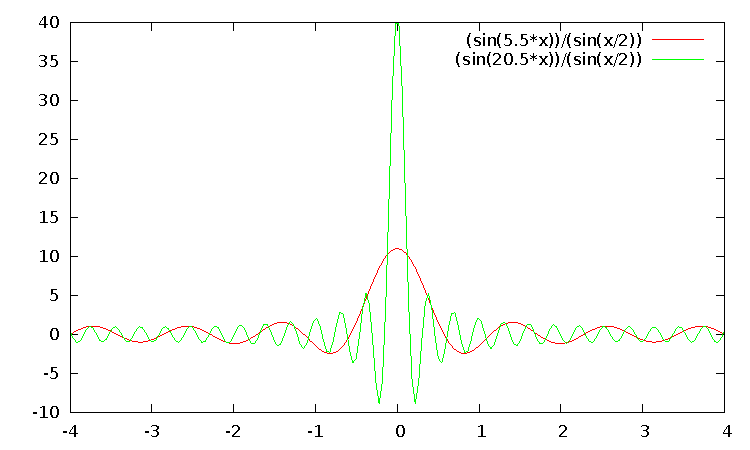
\includegraphics{dirich.pdf}
\end{center}

Note that the central peak will get taller and taller with $N$ being larger,
and the side peaks will stay small (but oscillate wildly).
Again, we are looking at in some sense an approximate delta function,
although it has
all these oscillations away from zero which do not go away.  So we expect that
$s_N$ goes to $f$.  Things are not so simple, but under some conditions on
$f$, such a conclusion holds.

People write
$$
\delta(x) \sim \sum_{n=\infty}^\infty e^{inx}
$$
although we can't say that as
we have not really defined the delta function, no a Fourier series of
whatever kind object it is.


\medskip

\textbf{Theorem 8.14:}
Let $x$ be fixed and let $f$ be Riemann integrable on $[-\pi,\pi]$.  Suppose that there exist $\delta > 0$ and $M$ such that
$$
\abs{f(x+t)-f(x)} \leq M \abs{t}
$$
for all $t \in (-\delta,\delta)$, then
$$
\lim_{N \to \infty} s_N(f;x) = f(x) .
$$

\medskip

In other words, if for example $f$ is differentiable at $x$
then we obtain convergence.  Generally what the result implies is
that if the function is continuous
piecewise smooth, then the Fourier series converges
(pointwise).   By continuous piecewise smooth we mean that $f$
is continuous and periodic so $f(-\pi) = f(\pi)$ and furthermore
that there are points $x_0 = -\pi < x_1 < \cdots < x_k = \pi$
such that $f$ restricted to $[x_j,x_{j+1}]$
is continuously differentiable (up to the endpoints) for all $j$.

\medskip

\begin{proof}
We notice that for all $N$ we get
\begin{equation*}
\frac{1}{2\pi} \int_{-\pi}^\pi D_N = 1 .
\end{equation*}
Write
\begin{equation*}
\begin{split}
s_N(f;x)-f(x) & =
\frac{1}{2\pi} \int_{-\pi}^\pi f(x-t) D_N(t) \, dt 
-
f(x)
\frac{1}{2\pi} \int_{-\pi}^\pi D_N(t) \, dt
\\
& = 
\frac{1}{2\pi} \int_{-\pi}^\pi \bigl( f(x-t) - f(x) \bigr) D_N(t) \, dt 
\\
& = 
\frac{1}{2\pi} \int_{-\pi}^\pi \frac{f(x-t) - f(x)}{\sin(t/2)} \sin\bigl(
(N+\nicefrac{1}{2})t \bigr) \, dt 
\end{split}
\end{equation*}
Now by the hypotheses we obtain that
for small nonzero $t$ we get
\begin{equation*}
\abs{ \frac{f(x-t) - f(x)}{\sin(t/2)} }
\leq
\frac{M\abs{t}}{\abs{\sin(t/2)}}
\end{equation*}
As $\sin(t) = t + h(t)$ where $\frac{h(t)}{t} \to 0$ as $t \to 0$,
we notice that
$\frac{M\abs{t}}{\abs{\sin(t/2)}}$ is continuous at the origin
and hence 
$\frac{f(x-t) - f(x)}{\sin(t/2)}$ must be bounded near the origin.
As $t=0$ is the only place on $[-\pi,\pi]$ where the denominator vanishes,
it is the only place where there could be a problem.  The function is
also Riemann integrable.  Now we use a trigonometric identity
that follows from the definition (and you've seen it on the homework
actually) that 
$$
\sin\bigl( (N+\nicefrac{1}{2})t \bigr)
=
\cos(t/2) \sin(Nt) + 
\sin(t/2) \cos(Nt)
$$
so
\begin{equation*}
\begin{split}
\frac{1}{2\pi} \int_{-\pi}^\pi \frac{f(x-t) - f(x)}{\sin(t/2)} \sin\bigl(
(N+\nicefrac{1}{2})t \bigr) \, dt 
=
&
\frac{1}{2\pi} \int_{-\pi}^\pi
\left( \frac{f(x-t) - f(x)}{\sin(t/2)}
\cos (t/2) \right) \sin (Nt) \, dt
\\
& +
\frac{1}{2\pi} \int_{-\pi}^\pi \bigl( f(x-t) - f(x) \bigr)
\cos (Nt) \, dt
\end{split}
\end{equation*}
Now 
$\frac{f(x-t) - f(x)}{\sin(t/2)} \cos (t/2)$
and
$\bigl( f(x-t) - f(x) \bigr)$ are bounded Riemann integrable functions
and so their Fourier coefficients go to zero by Theorem 8.12.  So the two
integrals on the right hand side, which compute the Fourier coefficients
for the real version of the Fourier series go to 0 as $N$ goes to infinity.
This is because $\sin(Nt)$ and $\cos(Nt)$ are also orthonormal systems.
with respect to the same inner product.
Hence $s_N(f;x)-f(x)$ goes to 0 and so $s_N(f;x)$ goes to $f(x)$.
\end{proof}

\medskip

In particular this has the following corollary:

\medskip

\textbf{Corollary:}
If $f(x) = 0$ on an entire open interval $J$, then $\lim s_N(f;x) = 0$
for all $x \in J$.

\medskip

In other words, if two functions $f$ and $g$
are equal on an open interval $J$, then the
points on $J$ where $\{ s_N(f;x) \}$ and $\{ s_N(g;x) \}$ converge are the same.  That is,
convergence at $x$ is only dependent on the values of the function
near $x$.

\medskip

We have seen Theorem 8.15 as an example for Stone-Weierstrass theorem.
That is, any continuous function on $[-\pi,\pi]$ can be uniformly approximated
by trigonometric polynomials.  However, these trigonometric polynomials need
not be the partial sums $s_N$.  On the other hand, (exercise 15) they can be
explicitly constructed from $s_N$.

\medskip

We have that the convergence always happens in the $L^2$ sense and
furthermore that formal operations on the (infinite) vectors of
Fourier coefficients is the same as the operations using the integral
inner product.

\medskip

We will mostly sketch out the proof and leave some details to the reader
as exercises.  Some of these are exercises in Rudin.

%FIXME: Should we prove $L^2$ triang and CS?  This is just formal nonsense

\medskip

\textbf{Theorem 8.16:} (Parseval)
Let $f$ and $g$ be Riemann integrable $2\pi$-periodic functions
with
$$
f(x) \sim
\sum_{n=-\infty}^\infty c_n e^{inx}
\qquad \text{and} \qquad
g(x) \sim
\sum_{n=-\infty}^\infty d_n e^{inx} .
$$
Then
$$
\lim_{N\to\infty} \snorm{f-s_N(f)}_2^2 = 
\lim_{N\to\infty}
\frac{1}{2\pi}
\int_{-\pi}^\pi
\abs{f(x)-s_N(f;x)}^2 \, dx
=0 .
$$
Also
$$
\langle f , g \rangle =
\frac{1}{2\pi}
\int_{-\pi}^\pi
f(x) \overline{g(x)}\, dx
=
\sum_{n=-\infty}^\infty c_n \overline{d_n} ,
$$
and
$$
\snorm{f}_2^2
=
\frac{1}{2\pi}
\int_{-\pi}^\pi
\abs{f(x)}^2 \, dx
=
\sum_{n=-\infty}^\infty \abs{c_n}^2.
$$

\medskip

We will skip the proof in lecture.

\begin{proof}
It is not hard too prove (Exercise 12 in chapter 6) that there is
a continuous $2\pi$-periodic function $h$ such that
$$
\snorm{f-h}_2 < \epsilon .
$$
Now we know that we can approximate $h$ with a trigonometric polynomial
uniformly, that is there is a trigonometric polynomial $P(x)$
such that
$\abs{h(x) - P(x)} < \epsilon$ for all $x$.
Hence
$$
\snorm{h-P}_2 \leq \epsilon.
$$
If $P$ is of degree $N_0$ then for all $N \geq N_0$ we have
$$
\snorm{h-s_N(h)}_2 \leq \snorm{h-P}_2 \leq \epsilon
$$
as $s_N(h)$ is the best approximation for $h$ in $L^2$ (Theorem 8.11).
Next by the inequality leading up to Bessel we have
$$
\snorm{s_N(h)-s_N(f)}_2
=
\snorm{s_N(h-f)}_2
\leq
\snorm{h-f}_2 \leq \epsilon
$$
It is not difficult (exercise 11 in chapter 6) to show the triangle
inequality for the $L^2$ norm, that is
$$
\snorm{f-s_N(f)}_2
\leq
\snorm{f-h}_2
+
\snorm{h-s_N(h)}_2
+
\snorm{s_N(h)-s_N(f)}_2
\leq 3\epsilon .
$$
For all $N \geq N_0$.

Next
$$
\langle s_N(f) , g \rangle
=
\frac{1}{2\pi}
\int_{-\pi}^\pi
s_N(f;x) \overline{g(x)} \, dx
=
\sum_{k=-N}^N
c_k 
\frac{1}{2\pi}
\int_{-\pi}^\pi
e^{ikx}
\overline{g(x)} \, dx
=
\sum_{k=-N}^N
c_k 
\overline{d_k}
$$
Next we need the Schwarz (or Cauchy-Schwarz)
inequality (left as exercise), that is
$$
{\abs{\int_a^b f\bar{g}}}^2
\leq
\left( \int_a^b \abs{f}^2 \right)
\left( \int_a^b \abs{g}^2 \right)
$$
This is left as an exercise.  It actually follows by purely formal
linear algebra using simple the idea that the integral gives an inner
product.
So
%Next let $M$ be such that $\abs{g(x)} \leq M$ for all $x$,
%($g$ is Riemann integrable so bounded)
$$
\abs{\int_{-\pi}^\pi f\bar{g} - \int_{-\pi}^\pi s_N(f)g}
=
\abs{\int_{-\pi}^\pi (f- s_N(f))g}
\leq
\int_{-\pi}^\pi \abs{f- s_N(f)}\, \abs{g}
\leq
{\left(\int_{-\pi}^\pi \abs{f- s_N(f)}^2 \right)}^{1/2}
{\left( \int_{-\pi}^\pi \abs{g}^2 \right)}^{1/2} .
$$
Now the right hand side goes to 0 as $N$ goes to infinity.
\end{proof}


%%%%%%%%%%%%%%%%%%%%%%%%%%%%%%%%%%%%%%%%%%%%%%%%%%%%%%%%%%%%%%%%%%%%%%%%%%%%%%
%%%%%%%%%%%%%%%%%%%%%%%%%%%%%%%%%%%%%%%%%%%%%%%%%%%%%%%%%%%%%%%%%%%%%%%%%%%%%%
%%%%%%%%%%%%%%%%%%%%%%%%%%%%%%%%%%%%%%%%%%%%%%%%%%%%%%%%%%%%%%%%%%%%%%%%%%%%%%

\chapter{Lebesgue integral} \label{lebesgue:chapter}

%\vspace*{-3in}
%{\large DRAFT~~~~DRAFT~~~~DRAFT~~~~DRAFT~~~~\today}
%\vspace*{2.508in}

%%%%%%%%%%%%%%%%%%%%%%%%%%%%%%%%%%%%%%%%%%%%%%%%%%%%%%%%%%%%%%%%%%%%%%%%%%%%%%

\section{FIXME}
\label{sec:FIXME}

\sectionnotes{FIXME lectures}

We will define a very powerful integral, far better than Riemann in the
sense that it will allow us to integrate pretty much every reasonable
function and we will also obtain strong convergence results.  That is
if we take a limit of integrable functions we will get an integrable
function and the limit of the integrals will be the integral of the limit
under very mild conditions.  We will focus only on the real line, although
the theory easily extends to more abstract contexts.

\medskip

In Riemann integral the basic block was a rectangle.  If we wanted to
integrate a function that was identically 1 on an interval $[a,b]$, then the
integral was simply the area of that rectangle, so $1 \times (b-a) = b-a$.
For Lebesgue integral what we want to do is to replace the interval with a
more general subset of the real line.  That is, if we have a set $S \subset
\R$ and we take the \emph{indicator function} or \emph{characteristic
function} $\chi_S$ defined by
$$
\chi_S (x) =
\begin{cases}
1 & \text{ if $x \in S$,} \\
0 & \text{ else.}
\end{cases}
$$
Then the integral of $\chi_S$ should really be equal to the area under the
graph, which should be equal to the ``size'' of $S$.

\medskip

\textbf{Example:}
Suppose that $S$ is the set of rational numbers between $0$ and $1$.  Let us
argue that its size is 0, and so the integral of $\chi_S$ should be 0.
Let $\{ x_1, x_2, \ldots \} = S$ be an enumeration
of the points of $S$.  Now for any $\epsilon > 0$
take the sets
$$I_j = (x_j - \epsilon 2^{-j-1}, 
x_j + \epsilon 2^{-j-1}),$$
then
$$
S \subset \bigcup_{j=1}^\infty I_j .
$$
The ``size'' of any $I_j$ should be $\epsilon 2^{-j}$, so it seems reasonable
to say that the ``size'' of $S$ is less than the sum of the sizes of the $I_j$'s.
At worst we are grossly overestimating; every $I_j$ contains
infinitely
many other points of $S$, so there is a lot of overlap.  So
$$
\text{``size of $S$''} \leq
\sum_{j=1}^\infty \text{ ``size of $I_j$''} =
\sum_{j=1}^\infty \epsilon 2^{-j} = \epsilon.
$$
So the ``size of $S$'' (whatever that concept should be) seems like it ought
to be 0.  And hence the integral of $\chi_S$ should be 0.

\medskip

So to begin, we want to have a way to ``measure'' sets.  We focus
only on the real numbers and so suppose we wish to measure subsets of the real
numbers.  We would like (our Christmas wish) to have a function
$$
m \colon \sP(\R) \to [0,\infty]
$$
that is a function that takes subsets of the real numbers
and gives nonnegative extended real numbers, such that 
$$
m(\emptyset) = 0
$$
and if $\{ S_j \}$ is a countable collection of pairwise disjoint sets then
$$
\sum_{j=1}^\infty m(S_j) = m\left( \bigcup_{j=1}^\infty S_j \right)
$$
It should also replicate what we normally think of size of intervals,
that is $m( (a,b) ) = m([a,b) ) = m([a,b]) = m((a,b]) = b-a$.

Unfortunately, such a function is impossible.  At least there is
no such function on all of $\sP(\R)$ (the power set of the reals).
We do have such a function on a subset of the powerset.  That is,
we will define a smaller set of subsets called measurable sets
and on these sets we will be able to define such a function.

So let's talk about certain collections of sets.  The collections we will
want are so called $\sigma$-algebras (Rudin talks about $\sigma$-rings, the
idea is very similar, I'll note what the difference is).

\medskip

\textbf{Definition:}
Let $X$ be a set.
A collection of sets $\sM \subset \sP(X)$ is a \emph{$\sigma$-algebra} if
\begin{enumerate}[(i)]
\item $\sM$ is nonempty,
\item $\sM$ is closed under complements, that is, if $A \in \sM$ then
$A^c = X \setminus A \in \sM$,
\item $\sM$ is closed under countable unions, that is if $\{ A_j \}$ is
a countable collection of sets in $\sM$ then
$$
\bigcup_{j=1}^\infty A_j \in \sM .
$$
\end{enumerate}
If $\sM$ is closed only under finite unions, then we say that $\sM$ is an
\emph{algebra}.

\medskip

Most of the time below we will assume that $X=\R$, so you might as well
think of subsets of the real line.

\medskip

Definition of $\sigma$-ring and ring is similar but only needs closure under
relative complements.  A $\sigma$-algebra is always a $\sigma$-ring, and a
$\sigma$-ring is a $\sigma$-algebra if it contains the whole
set $X$ as an element.

The sets in $\sM$ are usually called \emph{measurable sets}.  We will define a
certain function on the powerset and define a certain
$\sigma$-algebra on which it has the desired properties.  Our
$\sigma$-algebra will be so large that we will essentially be able to
integrate anything we want.  It will be very hard to come up with sets that
are not in our $\sigma$-algebra.

\medskip

%FIXME: used $\R^*$ in basic anal
We will work with the \emph{extended real numbers}
$\overline{\R} = \R \cup \{ -\infty, \infty \}$.  We have previously used
really only its order properties such as $-\infty < x < \infty$ for
all $x \in \R$.  Now we will also often use arithmetic on 
$\overline{\R}$.  We have to be careful as
$\overline{\R}$ will not be a field like $\R$.  In fact, some operations are
not even defined.  Let us define
\begin{align*}
& x \cdot \infty = \infty \qquad \text{for all $x > 0$} \\
& x \cdot \infty = -\infty \qquad \text{for all $x < 0$} \\
& x + \infty = \infty \quad \text{and} \quad x - \infty = -\infty \qquad
\text{for all $x \in \R$} \\
&
\frac{x}{\pm\infty} = 0
\qquad \text{for all $x \in \R$}
\end{align*}
and so on.  Everything that is not an indefinite form
$\infty - \infty$, $\frac{\pm \infty}{\pm \infty}$, or $0 \cdot \infty$
has an obvious definition.  It will be convenient for measure theory to define
$$
0 \cdot \infty = 0 .
$$
We will have to avoid $\infty - \infty$ and
$\frac{\pm \infty}{\pm \infty}$.

\medskip

\textbf{Definition:}
Let $\sM$ be a $\sigma$-algebra.  Let
$$
\mu \colon \sM \to \overline{\R} .
$$
We say $\mu$ is \emph{additive} if given $A, B \in \sM$,
disjoint ($A \cap B = \emptyset$) then
$$
\mu ( A \cup B) = \mu (A) + \mu(B) .
$$
We say $\mu$ is \emph{countably additive} if given $\{ A_j \}$ a collection
of sets in $\sM$ such that $A_j \cap A_k = \emptyset$ for all $j\not=k$, then
$$
\mu \left( \bigcup_{j=1}^\infty A_j \right) =
\sum_{j=1}^\infty \mu (A_j) .
$$
Of course the sums have to make sense, so usually we will assume that $\mu$
does not achieve both $-\infty$ and $\infty$.

We will say that $\mu$ is nonnegative or monotonic if $\mu(A) \geq 0$ for all $A \in \sM$.

We also say that
$\mu$ is \emph{countably subadditive} if for every collection
$\{ A_j \}$ we have
$$
\mu \left( \bigcup_{j=1}^\infty A_j \right) \leq
\sum_{j=1}^\infty \mu (A_j) .
$$

\medskip

It is not too hard to show that if $\mu$ is additive then $\mu(\emptyset) =
0$.  We also have additivity for arbitrary finite unions by induction.

If $B \subset A$ and $\mu(B)$ is finite, then
writing $A = B \cup (A\setminus B)$ we obtain that 
$$
\mu(A\setminus B) = \mu(A) - \mu(B) .
$$

Another useful property for additive functions is
$$
\mu(A \cup B) + \mu(A \cap B) = \mu(A) + \mu(B) .
$$
This follows by looking at the disjoint unions
$B = (B \setminus A) \cup (A \cap B)$ and noting that $A \cup B = A \cup (B
\setminus A)$.  So for example a nonnegative additive function is
also (finitely) subadditive:
$$
\mu(A \cup B) \leq \mu(A) + \mu(B) .
$$

Countably additive functions are additive of course.
Also, countably additive $\mu$ play nicely with limits.

\medskip

\textbf{Theorem 11.3:}
Suppose that $\mu$ is a countably additive function on a $\sigma$-algebra
$\sM$ and $A_1 \subset A_2 \subset \cdots$ are sets in $\sM$
and $A = \cup_j A_j$, then
$$
\lim_{n \to \infty} \mu(A_n) = \mu (A) ,
$$
where the limit has the obvious interpretation for $\infty$ (or $-\infty$).

\medskip

\begin{proof}
Write $B_1 = A_1$ and $B_j = A_j \setminus A_{j-1}$.
Then the $B_j$'s are pairwise disjoint and $A = \cup_j B_j$, so
$$
\mu(A) = \sum_{j=1}^\infty \mu(B_j) .
$$
As $A_n = B_1 \cup B_2 \cup \cdots \cup B_n$ then
$$
\mu(A_n) = \sum_{j=1}^n \mu(B_j) ,
$$
and the result follows.
\end{proof}

\medskip

\textbf{Definition:}
If we have a $\sigma$-algebra $\sM$ of measurable sets, then we call a
function
$$
\mu \colon \sM \to \overline{\R}
$$
a \emph{measure} if it is a nonnegative and countably additive.  Sometimes
$\mu(\emptyset) = 0$ is also given as requirement, but that follows from
additivity.  Also some authors require $\mu$ to not be identically zero.

\medskip

It turns out there are many different measures.  The simplest measure can be
defined as follows.  Let $\sM$ be all of $\sP(X)$, and define
$\mu(A) = \abs{A}$, the cardinality of $A$.  This $\mu$ is called the
\emph{counting measure}.  Despite how trivial this example
is, it does happen to be useful; we will see it later on.

\medskip

Let us construct the Lebesgue measure.  What we will actually construct
is a subadditive nonnegative function on all of $\sP(\R)$, which will turn out to be a
measure (so countably additive) on some large $\sigma$-algebra in $\sP(\R)$.

\medskip

Let us define a bounded interval to be a set of the form
$$
\{ x : a < x < b \}
\qquad \text{or} \qquad
\{ x : a \leq x < b \}
\qquad \text{or} \qquad
\{ x : a < x \leq b \}
\qquad \text{or} \qquad
\{ x : a \leq x \leq b \}
$$
for real numbers $a \leq b$.  We allow $a = b$, meaning we allow 
$\emptyset$ and the single point set $\{ x \}$ to also be intervals.
If $I$ is a bounded interval, define
$$
m(I) = b-a .
$$

%Let $\sE$ be the set of finite unions of pairwise disjoint intervals.  If $A = 
%I_1 \cup I_2 \cup \cdots \cup I_n$ is a pairwise disjoint union of intervals
%then define
%$$
%m(A) = m(I_1)+\cdots +m(I_n) .
%$$
%It is not hard to see that $m$ is well defined and
%that $m$ is a nonnegative additive function on the algebra $\sE$
%(not a $\sigma$-algebra).  Also $m$ is finite on $\sE$.
%Sets in $\sE$ are called elementary sets.
%
%\medskip
%
%We claim the function $m$ is a so-called \emph{regular} function on $\sE$.  That is,
%for any $A \in \sE$, and every $\epsilon > 0$ there are
%a closed set $F$ and an open set $G$ in $\sE$, with $F \subset A \subset G$
%such that
%$$
%m(G) - \epsilon \leq m(A) \leq m(F) + \epsilon .
%$$
%The claim follows by noting that the property is not hard to show for an
%interval.

It is easy to see that given any bounded interval $I$
and any $\epsilon > 0$, there are
a closed interval $F$ and an open interval $G$, with $F \subset A \subset G$
such that
$$
m(G) - \epsilon \leq m(I) \leq m(F) + \epsilon .
$$

Now the point is to show that we can extend $m$ to a countably additive
function on a $\sigma$-algebra that contains all the intervals.%$\sE$.

Let $E \subset \R$ be any set.  Let $\{ I_j \}$ be a countable
collection of bounded open intervals covering $E$,
that is
$$
E \subset \bigcup_{j=1}^\infty I_j .
$$
Define the \emph{outer measure}
as
$$
m^*(E) = \inf \sum_{j=1}^\infty m(I_j) ,
$$
where the $\inf$ is taken over all coverings of $E$ by countably many bounded open
intervals.

It is immediate that $m^*$ is nonnegative ($m^*(A) \geq 0$) and monotone (if $A \subset B$
then $m^*(A) \leq m^*(B)$).

\medskip

\textbf{Theorem 11.8:}
If $I$ is a bounded interval, then $m(I) = m^*(I)$.  Also $m^*$ is countably subadditive.

\medskip

That is $m^*$ is a countably subadditive extension of $m$.

\medskip

\begin{proof}
Suppose that $I$ is a bounded interval, and let $\epsilon > 0$ be given.
Then there exists an open bounded interval $G$, $I \subset G$, such that
$m(G) \leq m(I) + \epsilon$.
As $G$ is a covering of $I$ by bounded open intervals,
$$
m^*(I) \leq m(G) .
$$
So $m^*(I) \leq m(G) \leq m(I) + \epsilon$.  As $\epsilon > 0$
was arbitrary we have $m^*(I) \leq m(I)$.
By definition of $m^*$ there exists a sequence
of open bounded intervals $\{ G_j \}$ covering $I$ such that
$$
\sum_{j=1}^\infty m(G_j) \leq m^*(I) + \epsilon .
$$
There also exists a bounded closed interval $F$, $F \subset I$, such that
$m(F) \geq m(I)-\epsilon$.
As $F$ is compact, there is some $N$ such that
$$
F \subset G_1 \cup G_2 \cup \cdots \cup G_N .
$$
and so
$$
m(I) \leq \epsilon+m(F) \leq \epsilon + \sum_{j=1}^N m(G_j)
\leq 
\epsilon + \sum_{j=1}^\infty m(G_j) \leq m^*(I) + 2\epsilon .
$$
So $m(I) \leq m^*(I)$.  Thus $m(I) = m^*(I)$.

\medskip

Let us show countable subadditivity.
Suppose that $A = \cup_{j=1}^\infty A_j$.
If $m^*(A_j) = \infty$ for any $j$, then we are done, so suppose that
$m^*(A_j)$ is finite for every $j$.

Each $A_j$
has a covering $G_{jk}$ of bounded open intervals such that
$$
\sum_{k=1}^\infty m(G_{jk}) \leq m^*(A_j) + \epsilon 2^{-j} .
$$
So as all the $G_{jk}$ together cover $A$
$$
m^*(A)
\leq
\sum_{j=1}^\infty
\sum_{k=1}^\infty
m(G_{jk})
\leq
\sum_{j=1}^\infty
\Bigl( m^*(A_j) + \epsilon 2^{-j} \Bigr)
\leq
\left(
\sum_{j=1}^\infty
m^*(A_j) \right)
+ \epsilon .
$$
\end{proof}

Note that by the same argument as for the example we started the section
with, we have:

\medskip

\textbf{Corollary:}
If $S \subset \R$ is countable, then $m^*(S) = 0$.

\medskip

It will be useful to have the following result about open subsets of $\R$:

\medskip

\textbf{Proposition:}
An open subset $W \subset \R$ is a countable union of pairwise
disjoint open intervals.

\medskip

\begin{proof}
For each point $x \in W$, let $I_x$ be the largest open interval such
that $I_x \subset W$ and $x \in I_x$ (that is, $I_x$ is the union of all
open intervals contained in $W$ that contain $x$).  Every $I_x$ contains
rational points.  Furthermore if $y \in I_x$, then $I_y = I_x$.  So
$$
W = \bigcup_{x \in \Q \cap W} I_x
$$
We take some enumeration of the rationals and pick one rational
point in every $I_x$, then we have $W$ written as a countable union of
pairwise disjoint open intervals.
\end{proof}

\medskip

Here we depart a little from Rudin again to have a simpler definition:

\textbf{Definition:}
A set $E \subset \R$ is said to be \emph{Lebesgue measurable}
if for each subset $A \subset \R$ we get
$$
m^*(A) = m^*(A \cap E) + m^*(A \cap E^c) .
$$
We will denote the measurable sets by $\sM$.  And unless otherwise stated
(that is, when talking about Lebesgue measure $m$ or the associated outer
measure $m^*$) $\sM$ will mean Lebesgue measurable sets.

Note that
$$
m^*(A) \leq m^*(A \cap E) + m^*(A \cap E^c)
$$
is always true by subadditivity of $m^*$.  So to show that $E$ is measurable,
what we need to show is that
$$
m^*(A) \geq m^*(A \cap E) + m^*(A \cap E^c).
$$
Furthermore, this inequality is always true when $m^*(A) = \infty$, so
we only really need to worry about $A$ such that $m^*(A) < \infty$.

If $E$ is measurable then $E^c$ is measurable by symmetry of the
condition.  It is not hard
to see that $\emptyset$ and $\R$ are measurable.

\medskip

\textbf{Proposition:}
If $m^*(E) = 0$, then $E$ is Lebesgue measurable.

\medskip

\begin{proof}
For any set $E$ we have
$$
m^*(A \cap E) \leq m^*(E)
$$
so $m^*(A \cap E) = 0$.  Also
$$
m^*(A \cap E^c) \leq m^*(A) .
$$
So
$$
m^*(A \cap E) + m^*(A \cap E^c) \leq m^*(A) .
$$
\end{proof}

\medskip

So for example countable sets and their complements are Lebesgue measurable.

\medskip

Sets of measure 0 are called \emph{null sets}.  We have seen above that all
countable subsets of $\R$ are null sets, but there exist 
uncountable null sets as well.

\medskip

\textbf{Proposition:}
The set of Lebesgue measurable sets
$\sM$ is an algebra of sets.

\medskip

\begin{proof}
As we said above, $\sM$ is closed under complements.  So we need to show that
it is closed under finite unions.

Let $E$ and $F$ be measurable.
Given any $A$ we have
$$
m^*(A \cap E^c) =
m^*(A \cap E^c \cap F) +
m^*(A \cap E^c \cap F^c)
=
m^*(A \cap E^c \cap F) +
m^*\bigl(A \cap ( E \cup F)^c \bigr)
$$
%and
%$$
%m^*(A \cap F^c) =
%m^*(A \cap F^c \cap E) +
%m^*(A \cap F^c \cap E^c)
%=
%m^*(A \cap E \cap F^c ) +
%m^*(A \cap ( E \cup F)^c ).
%$$
and
$$
m^*(A \cap E^c)
=
m^*(A) -
m^*(A \cap E) .
$$
Also
$A \cap (E \cup F) = (A \cap E) \cup (A \cap E^c \cap F)$ so
$$
m^*\bigl(A \cap (E \cup F) \bigr)
\leq
m^*(A \cap E ) +
m^*(A \cap E^c \cap F ) .
$$
Hence,
\begin{equation*}
\begin{split}
m^*\bigl(A \cap (E \cup F) \bigr) +
m^*\bigl(A \cap (E \cup F)^c \bigr)
& =
m^*\bigl(A \cap (E \cup F) \bigr) +
m^*(A \cap E^c ) -
m^*(A \cap E^c \cap F )
\\
& =
m^*(A)
+
m^*\bigl(A \cap (E \cup F) \bigr)
-
m^*(A \cap E ) -
m^*(A \cap E^c \cap F )
\\
& \leq
m^*(A) .
\end{split}
\end{equation*}
\end{proof}

\medskip

\textbf{Proposition:}
Let $E_1, \ldots, E_n$ be pairwise disjoint and measurable, then
for any set $A$ we have
$$
m^*\left( A \cap \left( \bigcup_{j=1}^n E_j \right) \right)
=
\sum_{j=1}^n
m^*( A \cap  E_j ) .
$$

\medskip

\begin{proof}
The set $E_n$ is measurable and hence
\begin{equation*}
\begin{split}
m^*\left( A \cap \left( \bigcup_{j=1}^n E_j \right) \right)
& =
m^*\left( A \cap \left( \bigcup_{j=1}^n E_j \right) \cap E_n \right)
+
m^*\left( A \cap \left( \bigcup_{j=1}^n E_j \right) \cap E_n^c \right)
\\
& =
m^*( A \cap E_n )
+
m^*\left( A \cap \left( \bigcup_{j=1}^{n-1} E_j \right) \right)
\end{split}
\end{equation*}
and the proof follows by induction.
\end{proof}

\medskip

\textbf{Theorem:}
The set of Lebesgue measurable sets is a $\sigma$-algebra.

\medskip

\begin{proof}
Suppose that $E = \cup_{j=1}^\infty E_j$ where all the $E_j$
are measurable.  Define $F_1 = E_1$ and
$F_j = E_j \setminus \cup_{k=1}^{j-1} E_{k}$.  We have that $F_j$
is measurable for every $j$ as $\sM$ is an algebra.  We have that $F_j \cap F_k = \emptyset$
if $j \not= k$, and also that $E = \cup_{j=1}^\infty F_j$.

Let $A$ be any set.  Then,
\begin{equation*}
\begin{split}
m^*(A)
& =
m^*\left(A \cap \bigcup_{j=1}^n F_j\right)
+
m^*\left(A \cap {\left(\bigcup_{j=1}^n F_j\right)}^c\,\right)
\\
& \geq
m^*\left(A \cap \bigcup_{j=1}^n F_j\right)
+
m^*(A \cap E^c)
\\
& =
\sum_{j=1}^n
m^*(A \cap F_j)
+
m^*(A \cap E^c) .
\end{split}
\end{equation*}
Taking limits we have
\begin{equation*}
\begin{split}
m^*(A)
\geq
\sum_{j=1}^\infty
m^*(A \cap F_j)
+
m^*(A \cap E^c)
\geq
m^*\left(A \cap \bigcup_{j=1}^\infty F_j\right)
+
m^*(A \cap E^c)
=
m^*(A \cap E)
+
m^*(A \cap E^c) .
\end{split}
\end{equation*}
So $E$ is measurable.
\end{proof}

\medskip

\textbf{Theorem:}
All intervals are Lebesgue measurable, and hence all open sets are
measurable.

\medskip

\begin{proof}
Let $I$ be an interval of the form
$(-\infty,x)$, $(-\infty,x]$,
$(x,\infty)$, or $[x,\infty)$.
Let $\epsilon > 0$ be given and
$A$ be an arbitrary set such that
$m^*(A) < \infty$.  Let $\{ I_n \}$
be a countable collection of open bounded intervals such that
$$
A \subset \bigcup_{j=1}^\infty I_j ,
$$
and such that
$$
\sum_{j=1}^\infty m(I_j) \leq m^*(A) + \epsilon .
$$
Note that $I_j \cap I$ and
$I_j \cap I^c$ are bounded intervals (could be empty).
We have
\begin{align*}
m^*(A \cap I)
& \leq
\sum_{j=1}^\infty m(I_j \cap I) , \qquad \text{and}
\\
m^*(A \cap I^c)
& \leq
\sum_{j=1}^\infty m(I_j \cap I^c) .
\end{align*}
We have that $m(I_j) = m(I_j \cap I) + m(I_j \cap I^c)$.
So
$$
m^*(A \cap I)
+
m^*(A \cap I^c)
\leq
\sum_{j=1}^\infty m(I_j)
\leq m^*(A) + \epsilon .
$$
As $\epsilon > 0$ was arbitrary we obtain the required inequality.
If $m^*(A) = \infty$ the inequality was trivial.

Any bounded interval is an intersection of two half infinite intervals as
above, and so is measurable.
Any open set is a countable union of open intervals, and so it is also
measurable.
\end{proof}

\medskip

We of course also get that all closed sets are measurable.  But we get a lot
more.  We get that countable unions of closed sets are measurable, and so are
countable intersections of open sets, and so on and so forth.

It is not hard to prove that an intersection of $\sigma$-algebras is
still a $\sigma$-algebra.  Therefore, there exists a smallest
$\sigma$-algebra that contains the open sets (it's the intersection of all
$\sigma$-algebras containing the open sets).  This $\sigma$-algebra
is denoted by $\sB$ and the sets in it are called
the \emph{Borel sets}.  As $\sB \subset \sM$, we have that all Borel sets
are measurable.  Sometimes it is just convenient to talk about
$\sB$ rather than $\sM$.

\medskip

Let us now define 
$$
m \colon \sM \to [0,\infty]
$$
by defining $m(E) = m^*(E)$.  As $m^*$ agreed with the earlier definition of
$m$ on intervals,
this new $m$ agrees with our earlier definition of $m$ (on intervals).
We have still not shown that $m$ is a measure on $\sM$.
We call $m$ the \emph{Lebesgue measure} (we will show momentarily that it
really is a measure, so the name is justified).

\medskip

\textbf{Theorem (like 11.10 in Rudin):}
$m$ is countably additive, and hence a measure.

\medskip

\begin{proof}
Let $\{E_j\}$ be a family of pairwise disjoint Lebesgue measurable sets
and let $E = \cup_{j=1}^\infty E_j$.
If $m(E_j) = \infty$ for any $j$, then $m(E) = \infty$ and additivity
is trivial.  So assume that
$m(E_j) < \infty$ for all $j$.

Using $A=\R$ with an above proposition we have for any $n$
$$
m( E)
=
m\left( \bigcup_{j=1}^\infty E_j  \right)
\geq
m\left( \bigcup_{j=1}^n E_j  \right)
=
\sum_{j=1}^n
m( E_j ) .
$$
Taking limits we have
$$
m( E)
\geq
\sum_{j=1}^\infty
m( E_j ) .
$$
The opposite inequality follows by subadditivity.
\end{proof}

\medskip

\textbf{Proposition:}
If $E \subset \R$ is Lebesgue measurable, then for every $\epsilon > 0$
there exist an open set $G$ and a closed set $F$
such that $F \subset E \subset G$,
$$
m(E \setminus F) < \epsilon , \qquad \text{and} \qquad
m(G \setminus E) < \epsilon .
$$

\medskip

\begin{proof}
If $m(E) < \infty$ then $G$ is found directly by definition of $m^*$.
If $m(E) = \infty$, then we have to work a little harder.  So look at the
sets $E_j = E \cap [j,j+1)$.  We have that $m(E_j) \leq m\bigl([j,j+1)\bigr)
< 1 < \infty$, and $E = \cup_{j=-\infty}^\infty E_j$.  For every $j$ we can find an open set
$G_j$ such that, $E_j \subset G_j$ and $m(G_j \setminus E_j) < \epsilon
2^{-\abs{j}}$.
Let $G = \cup_{j=-\infty}^\infty G_j$.
So
$$
m(G \setminus E)
=
m\left( \bigcup_{j=-\infty}^\infty ( G_j\setminus E) \right)
\leq
m\left( \bigcup_{j=-\infty}^\infty ( G_j\setminus E_j) \right)
\leq
\sum_{j=-\infty}^\infty
m( G_j\setminus E_j)
<
\sum_{j=-\infty}^\infty
\epsilon 2^{-\abs{j}}
=
3\epsilon .
$$

Then to
find $F$, take the complement $E^c$ and find an open set that covers it
and take a complement of that.  Details are left to student.
\end{proof}

\medskip

We remark that by letting $\epsilon$ go to 0, we can show (left to
students) that there exists a Borel set $G$ that is a countable intersection
of open sets, and a Borel set $F$ that is a countable union of closed sets,
such that $F \subset E \subset G$
$$
m(E \setminus F) = m(G \setminus E) = 0 .
$$
Note that, of course, $m(E)=m(F)=m(G)$.
So every Lebesgue measurable set is almost like a Borel set; the difference
is a null set.
 
\medskip

\textbf{Measurable functions}

\medskip

If we want to integrate functions, we want to know which functions play
nicely with the measure, or actually with the measurable sets.
For example if $S$ is a nonmeasurable set, then we don't expect
to be able to integrate the characteristic function $\chi_S$, as its integral
should be the measure of $S$.

\medskip

Let us work in a general \emph{measurable space}
$(X,\sM)$, that is, a set $X$ and a $\sigma$-algebra of sets $\sM$.
If you want to, you can think of $(\R,\sM)$, where $\sM$ are the Lebesgue
measurable sets.  Note that we will not worry about the actual measure.

\medskip

\textbf{Definition 11.13:}
Let $(X,\sM)$ is a measurable space.  $f \colon X \to \overline{\R}$ is said
to be \emph{measurable} %(or measurable with respect to $\sM$)
if
$$
f^{-1} \bigl( (a,\infty] \bigr)
=
\{ x \in X : f(x) > a \}
\in \sM
$$
for all $a \in \R$.

\medskip

If $X=\R$ and $\sM$ is the set of Lebesgue measurable sets, then
we say that $f$ is said to be \emph{Lebesgue measurable}.  If $X=\R$ and
$\sM =\sB$ is the $\sigma$-algebra of Borel sets, then
$f$ is said to be \emph{Borel measurable}.  Note that if a function is
Borel measurable then it is, of course, Lebesgue measurable.

When people speak of just ``measurable'' functions on the real line, they will
generally mean Lebesgue measurable.

\medskip

\textbf{Proposition:}
If $f \colon \R \to \R$ is continuous, then 
it is Borel measurable
(and hence Lebesgue measurable).

\medskip

\begin{proof}
The interval $(a,\infty)$ is open and so
$f^{-1}\bigl( (a,\infty) \bigr)$ is open and so Borel (and so Lebesgue
measurable as well).
\end{proof}

\medskip

\textbf{Theorem 11.15:}
Let $(X,\sM)$ is a measurable space and $f \colon X \to \overline{\R}$ 
a function.
The following are equivalent:
\begin{enumerate}[(i)]
\item $f$ is measurable, that is $\{ x \in X : f(x) > a \}$ is measurable for
all $a \in \R$.
\item $\{ x \in X : f(x) \geq a \}$ is measurable for all $a \in \R$.
\item $\{ x \in X : f(x) < a \}$ is measurable for all $a \in \R$.
\item $\{ x \in X : f(x) \leq a \}$ is measurable for all $a \in \R$.
\end{enumerate}

\medskip

\begin{proof}
The implications (i) implies (ii) implies (iii) implies (iv) implies (i)
are shown by the following equalities:
\begin{align*}
& \{ x \in X : f(x) \geq a \} = \bigcap_{n=1}^\infty
\{ x \in X : f(x) > a - \nicefrac{1}{n} \} ,
\\
&
\{ x \in X : f(x) < a \} = X \setminus \{ x \in X : f(x) \geq a \} ,
\\
&
\{ x \in X : f(x) \leq a \} = \bigcap_{n=1}^\infty
\{ x \in X : f(x) < a  + \nicefrac{1}{n} \} ,
\\
&
\{ x \in X : f(x) > a \} = X \setminus \{ x \in X : f(x) \leq a \} .
\end{align*}
\end{proof}

\medskip

Similarly we also can prove that $f^{-1} (\{\infty\})$ and
$f^{-1}(\{-\infty\})$ are measurable.  So we could let $a$ vary over all of
$\overline{\R}$.

\medskip

\textbf{Theorem 11.16 (and corollary):}
Let $(X,\sM)$ is a measurable space and $f \colon X \to \overline{\R}$
and $g \colon X \to \overline{\R}$ are measurable then
\begin{enumerate}[(i)]
\item $\abs{f}$ is measurable.
\item $\max(f,g)$ and $\min(f,g)$ are measurable.
\item $f^+ = \max(f,0)$ and $f^-=-\min(f,0)$ are measurable.  (Note that
$f = f^+ - f^-$ and $\abs{f} = f^+ + f^-$)
\end{enumerate}

\begin{proof}
First item follows by
$
\{ x : \abs{f(x)} < a \} = \{ x : f(x) < a \} \cap \{ x : f(x) > -a \}
$

Second item follows by writing
$
\{ x : \max(f,g) (x) < a \} = \{ x : f(x) < a \} \cap \{ x : g(x) < a \}
$
and
$
\{ x : \min(f,g) (x) < a \} = \{ x : f(x) < a \} \cup \{ x : g(x) < a \}
$.

Last item follows by the second item.
\end{proof}

\medskip

In fact essentially any reasonable (see below about composition) operation we do to measurable functions
lands us back in the set of measurable functions.

\medskip

\textbf{Theorem 11.17:}
Let $(X,\sM)$ is a measurable space and
let $\{ f_n \}$ be a sequence of measurable functions defined on $X$.  
Define
\begin{align*}
& g_1(x) = \sup_{n \in \N} f_n(x) , \\
& g_2(x) = \inf_{n \in \N} f_n(x) , \\
& g_3(x) = \limsup_{n \to \infty} f_n(x) , \\
& g_4(x) = \liminf_{n\to\infty} f_n(x) .
\end{align*}
Then $g_1$, $g_2$, $g_3$, and $g_4$ are all measurable.   In particular, if
$\{f_n\}$ converges pointwise to $f$, then $f$ is measurable.

\medskip

\begin{proof}
If $g_1(x) > a$, then there is some $n$ such that
$f_n(x) > a$.  Similarly, if $f_n(x) > a$ for some $n$,
then obviously $g_1(x) > a$.  So
$$
\{ x : g_1(x) > a \}
=
\{ x : \sup_{n \in \N} f_n(x) > a \}
= \bigcup_{n=1}^\infty \{ x : f_n(x) > a \} .
$$
In other words $g_1$ is measurable.

Similarly,
$$
\{ x : g_2(x) < a \}
=
\{ x : \inf_{n \in \N} f_n(x) < a \}
= \bigcup_{n=1}^\infty \{ x : f_n(x) < a \} .
$$
So $g_2$ is measurable.

Next notice that
\begin{align*}
& g_3(x) =
\limsup_{n \to \infty} f_n(x)
=
\inf_{m \in \N} \left( \sup_{n \geq m} f_n(x) \right) ,
\\
& g_4(x) =
\liminf_{n \to \infty} f_n(x)
=
\sup_{m \in \N} \left( \inf_{n \geq m} f_n(x) \right) .
\end{align*}
So $g_3$ and $g_4$ are also measurable.

If the sequence is convergent, then limit is equal to limsup (or liminf) and
hence $f$ is measurable.
\end{proof}

Composition is somewhat tricky.  Even if $f \colon \R \to \R$ and
$g \colon \R \to \R$ are Lebesgue
measurable, doesn't mean that $f \circ g$ is measurable.
First we notice that what really happens is that a Lebesgue
measurable function
is a function that takes Borel sets on $\R$ into Lebesgue measurable
sets, that is, if $A$ is a Borel set
then $g^{-1}(A)$ is Lebesgue measurable.
The inverse image of a Lebesgue measurable set need not be Lebesgue measurable
for a Lebesgue measurable function.  We would need something stronger:

\medskip

\textbf{Proposition:}
If $f \colon \R \to \R$ and
$g \colon \R \to \R$ are both Borel measurable, then $f \circ g$
is Borel measurable.

\medskip

The proof is left to student.
%You can also prove that if $f$
%is Borel measurable and $g$ is Lebesgue measurable then
%$f \circ g$ is Lebesgue measurable.
On the other hand there exist
examples of even a continuous $g$ and Lebesgue measurable $f$
so that $f \circ g$ is not Lebesgue measurable.

\medskip

\textbf{Theorem 11.18:}
Let $(X,\sM)$ is a measurable space,
$f \colon X \to \R$ and $g \colon X \to \R$ be measurable functions,
and $F \colon \R^2 \to \R$ be a continuous function, then
$h(x) = F\bigl(f(x),g(x)\bigr)$ is a measurable function.

In particular $f+g$ and $fg$ are measurable.

\medskip

\begin{proof}
Fix $a \in \R$, then look at the open set
$$
G = \{ (y_1,y_2) : F(y_1,y_2) > a \} .
$$
An open set contains a whole ball around every 
point.  So for every point $y=(y_1,y_2)$ in $G$
there is a $\delta > 0$ such that
$$
\{ (z_1,z_2) : y_1 - \delta < z_1 < y_1 +\delta, ~
y_2 - \delta < z_2 < y_2 +\delta \} \subset G .
$$
Since $\R^2$ contains a dense countable subset (the set of points with
rational coordinates), there are countably
many such sets whose union is $G$.  That is, there exist
sequences $\{ a_n\}$, $\{b_n\}$, $\{c_n\}$, and $\{d_n\}$ and
$$
I_n = \{ (z_1,z_2) : a_n < z_1 < b_n, 
c_n < z_2 < d_n \} ,
$$
such that
$$
G = \bigcup_{n=1}^\infty I_n .
$$
Then
\begin{equation*}
\begin{split}
\{ x : h(x) > a \} & =
\{ x : (f(x),g(x)) \in G \}
\\
& =
\bigcup_{n=1}^\infty
\{ x : a_n < f(x) < b_n, ~c_n < g(x) < b_n \}
\\
& =
\bigcup_{n=1}^\infty
\bigl(
\{ x : a_n < f(x) \}
\cap
\{ x : f(x) < b_n \}
\cap
\{ x : c_n < g(x) \}
\cap
\{ x : g(x) < b_n \} \bigr).
\end{split}
\end{equation*}
And so $\{ x : h(x) > a \}$ is measurable.
\end{proof}

\medskip

Let us motivate what we will do next.  For Riemann integral (using the
Darboux approach) we really took
step functions that were less than the function, integrated those and took
their supremum (that was the lower Darboux integral).  A step function is
a function that is constant on intervals, that is a function such that if
$I_1, I_2, \ldots, I_n$ are disjoint intervals and $c_1, \ldots, c_n$
are numbers then a step function is a function of the form
$$
s(x) = \sum_{j=1}^n c_j \chi_{I_j} (x) ,
$$
where $\chi_{I_j}$ is the characteristic function of $I_j$ (the function
that is 1 on $I_j$ and 0 elsewhere).  The integral of $s$ was easy to
define then
$$
\int s(x) \, dx = \sum_{j=1}^n c_j m(I_j) ,
$$
and $m(I_j)$ is just the length of the $j$th interval.
Then if we take the supremum of those sums, that is the integrals of those step
functions less than $f$, we get the integral of $f$.

For the Lebesgue approach we will do something very similar, except that
we now know how to measure a lot more sets, so we we can replace the $I_j$
with arbitrary measurable sets.  Let us first see what we replace the step
function with.

\medskip

\textbf{Definition:}
Let $(X,\sM)$ is a measurable space.
A function $s \colon X \to \R$ is said to be a \emph{simple function}
if the range is finite.  In other words, $s$ is simple if
it attains only finitely many values.

\medskip

Suppose that $s$ is a simple function and $s(X) = \{ c_1, c_2, \ldots, c_n
\}$.  Then let
$$
E_j = \{ x : s(x) = c_j \} ,
$$
and we can write
$$
s(x) = \sum_{j=1}^n c_j \chi_{E_j} (x) ,
$$
where $\chi_{E_j}$ is the characteristic function of $E_j$ (the function
that is 1 on $E_j$ and 0 elsewhere).
We note that $s$ is measurable if and only if $E_1$, $E_2$, \ldots, $E_n$
are measurable.

Be careful though, just because $s$ has this form and is measurable
doesn't mean that the $E_j$ are measurable.  For example if
$E$ is a nonmeasurable set then $1 = \chi_E + \chi_{E^c}$, which is a
measurable simple function.
The reason we made the ``if and only if'' statement is because the $c_j$
are all distinct numbers and the $E_j$ are disjoint.

It turns out that every function can be approximated by simple functions.

\medskip

\textbf{Theorem 11.20:}
Let $(X,\sM)$ is a measurable space.
Let $f \colon X \to \R$ be a function.  Then there is a sequence
$\{ s_n \}$ of simple functions converging pointwise to $f$.
If $f \geq 0$, we can choose $\{ s_n \}$ to be monotonically
increasing, that is $\{ s_n(x) \}$ is a monotonically increasing sequence
for every $x$.
Finally, if $f$ is measurable, then we can choose all the $s_n$ to be
measurable.

\medskip

\begin{proof}
First 
suppose that $f \geq 0$ and define for each $n \in \N$, and all
$j=1,2,\ldots,n2^n$, define
$$
E_{n,j}
=
\left\{ x : \frac{j-1}{2^n} \leq f(x) < \frac{j}{2^n} \right\} ,
$$
and
$$
F_n = \{ x : f(x) \geq n \} .
$$
Let
$$
s_n
=
\sum_{j=1}^{n2^n}
\frac{j-1}{2^n} \chi_{E_n,j}
\,
+
\,
n
\chi_{F_n} .
$$
A moment's reflection will show that $\{ s_n(x) \}_{n=1}^\infty$ really does converge
to $f(x)$.  Furthermore, by construction all the sets
are measurable if $f$ is measurable.

Finally if $f$ is not nonnegative, write $f = f^+ - f^-$ and
apply the above construction to $f^+$ and $f^-$ separately.
\end{proof}

Note that in the proof, if the function $f$ is bounded, then
beyond a certain $n$, the $F_n$ are all empty.  Then we must be at most
$2^{-n}$ from the value.  That means that the sequence $s_n$ converges
uniformly to $f$ in this case (only if $f$ is bounded).

\medskip

\textbf{The integral}

\medskip

Let $X$ be a set and
$\sM$ a $\sigma$-algebra, and $\mu$ a measure.
The triple $(X,\sM,\mu)$ is then called
a \emph{measure space}.
We will from now work in such an abstract measure space.
Again, if you wish, you can
just think of $X=\R$, $\sM$ the Lebesgue measurable sets and $\mu=m$, the
Lebesgue measure, but most of what we prove will work for an arbitrary
measure space.

\textbf{Definition:}
Suppose that
$$
s(x) = \sum_{j=1}^n c_j \chi_{E_j} (x)
$$
is measurable (and all the $E_j$'s are measurable) and suppose that $c_j >
0$.  Then define
$$
\int s\, d\mu =
\sum_{j=1}^n c_j \mu(E_j) .
$$
Given a measurable nonnegative function $f$, let $\sS$ be the set
of measurable nonnegative simple functions $s$ such that $0 \leq s \leq f$
$$
\int f\, d\mu = \sup_{s \in \sS} \int s\, d\mu .
$$
We leave it to the student to check that this is well defined if $f$ is a simple
function.
We call $\int f \,d\mu$ the \emph{Lebesgue integral} with respect to $\mu$.
We sometimes write
$$
\int f(x) \,d\mu(x) ,
$$
in case the variable is important.  If the set $X$ needs to be emphasized
we write
$$
\int_X f\, d\mu .
$$
And for a measurable subset $E$ we can define
$$
\int_E f\, d\mu = \int f \chi_E\, d\mu .
$$

In the special case of Lebesgue measure we may write
$$
\int_{-\infty}^\infty f(x)\, dx = \int_\R f\, dm ,
\qquad
\int_a^b f(x)\, dx = \int_{[a,b]} f\, dm .
$$
We will later prove that the notation is justified as we will obtain
the same values as the Riemann integral for Riemann integrable functions.

Also note that we could take $X \subset \R$ to be a measurable subset, and then we could let
$\mu$ be the restriction of $m$ to the measurable subsets of $X$.  Then
$$
\int_X f|_X \, d\mu
=
\int_\R f \chi_X \, dm ,
$$
where one integral exists if and only if the other one does.

\medskip

\textbf{Definition:}
For an arbitrary measurable function $f$ write $f = f^+-f^-$ and if at least
one of the integrals
$$
\int f^+\, d\mu \qquad \text{and} \qquad
\int f^-\, d\mu 
$$
is finite, we define
$$
\int f\, d\mu =
\int f^+\, d\mu - \int f^-\, d\mu  .
$$
If both 
$\int f^+\, d\mu$ and $\int f^-\, d\mu$ are finite then we
say $f$ is \emph{integrable} (or \emph{summable}) or perhaps
more precisely $f$ is Lebesgue integrable with respect to $\mu$ and we
write $f \in L^1(\mu)$ or $f \in L^1(X,\mu)$.  If $E \subset X$ is
measurable, then $L^1(E,\mu)$ has the obvious meaning.
We may write $L^1$ or $L^1(X)$ if the measure is clear from context.
%When the measure is the Lebesgue
%measure we might just write $L^1$, or perhaps $L^1(\R)$.

Note that we require both of the integrals to be finite to say integrable.

\medskip

\textbf{Proposition:}
\begin{enumerate}[(i)]
\item If $a \leq f(x) \leq b$ for all $x \in E$ and $\mu(E) < \infty$, then
$$
a \mu(E) \leq \int_E f\, d\mu \leq b \mu(E) .
$$
In particular, if $\mu(E) < \infty$ and a real-valued $f$ is bounded on $E$, then $f \in
L^1(E,\mu)$.
\item Suppose that $f, g$ are either integrable or $f,g$ are nonnegative and measurable.  If $f(x) \leq g(x)$ for all $x$, then
$$
\int f \, d\mu \leq \int g \, d\mu .
$$
\item If $f \geq 0$ is measurable, and $A$ and $B$ are
disjoint and measurable then
$$
\int_{A \cup B} f \, d\mu =
\int_{A} f \, d\mu +
\int_{B} f \, d\mu.
$$
\end{enumerate}

\medskip

\begin{proof}
For part (i) note that $a \chi_E(x) \leq f(x) \chi_E(x) \leq b
\chi_E(x)$ and $a \chi_E$ and $b \chi_E$ are simple functions.
Without loss of generality assume that $E = X$.
If $a \geq 0$, then $f = f^+$ and $f^- = 0$,
and also $a \leq f$.  So the first inequality follows.
Any simple function less than $f$ is also
less than $b$ showing the second inequality.  The cases $b \leq 0$
and $a < 0 < b$ follow similarly.

Part (ii) can be proved by noting that $f^+ \leq g^+$ and
$f^- \geq g^-$.  So we only need to prove the result for nonnegative
measurable functions.  If $s$ is simple and $s \leq f$, then $s \leq g$ and
the result follows.

Let us prove part (iii).
Let $s \leq f \chi_{A \cup B}$ be a nonnegative measurable simple
function $s = \sum_{j=1}^n c_j \chi_{E_j}$ then
$$
\int_{A \cup B} s \, d\mu
=
\sum_{j=1}^n c_j \mu(E_j)
=
\sum_{j=1}^n c_j \mu(E_j \cap A)
+
\sum_{j=1}^n c_j \mu(E_j \cap B)
=
\int_A s \, d\mu
+
\int_B s \, d\mu .
$$
Note that if $0 \leq s \leq f \chi_{A\cup B}$ then $s\chi_A \leq f\chi_A$
and $s\chi_A \leq f\chi_A$.  Therefore taking suprema over all such $s$
we get
$$
\int_{A \cup B} f \, d\mu
\leq
\int_A f \, d\mu
+
\int_B f \, d\mu .
$$
If $\int_A f \, d\mu = \infty$ or
$\int_B f \, d\mu = \infty$, then $\int_{A\cup B} f \, d\mu = \infty$ and
equality follows.  So let's assume that all 3 are finite.  Given $\epsilon >
0$ find a measurable simple $s\leq f \chi_{A\cup B}$ such that
$$
\int_A s \, d\mu
\geq
\int_A f \, d\mu - \epsilon
\qquad \text{and} \qquad
\int_B s \, d\mu 
\geq
\int_B f \, d\mu - \epsilon .
$$
This is not hard to do as $A$ and $B$ are disjoint, so just find $s_1$ that
works on $A$ (and is zero outside of $A$) and $s_2$ that works for $B$ (and
is zero outside of $B$) and let $s = s_1 + s_2$.
Then
$$
\int_{A \cup B} f \, d\mu
\geq
\int_{A \cup B} s \, d\mu
=
\int_A s \, d\mu
+
\int_B s \, d\mu 
\geq
\int_A f \, d\mu
+
\int_B f \, d\mu
- 2 \epsilon .
$$
\end{proof}

\medskip

Let us integrate complex valued functions.

\medskip

\textbf{Definition:}
Suppose that $f \colon X \to \C$ is a function.
If $f = u+iv$ where $u$ and $v$ are real-valued, then we say
that $f$ is \emph{measurable} if $u$ and $v$ are.

If $u$ and $v$ are integrable, then we say that $f$ is \emph{integrable}
and we write
$$
\int f \, d\mu = \int u \,d\mu + i \int v \,d\mu .
$$

\medskip

Note that
if $f$ is measurable then $\abs{f} = \sqrt{u^2+v^2}$ is also measurable.

In general when we write $L^1(X,\mu)$ from now on we will mean complex valued
functions.  It turns out there is no loss in generality by not allowing the
values $\pm\infty$ for integrable functions.  The set where an $L^1$
function could be $\infty$ must be a null set.

\medskip

\textbf{Proposition:}
\begin{enumerate}[(i)]
\item 
If $\mu(E) < \infty$ and $f \colon X \to \C$ is measurable and bounded on $E$, then $f \in
L^1(E,\mu)$.
\item If $f \in L^1(\mu)$ and $A$ and $B$ are
disjoint and measurable, then
$$
\int_{A \cup B} f \, d\mu =
\int_{A} f \, d\mu +
\int_{B} f \, d\mu.
$$
\item If $f \in L^1(\mu)$ and $c \in \C$, then $cf \in L^1(\mu)$ and
$$
\int cf \, d\mu = c \int f \, d\mu .
$$
\item If $\mu(E) = 0$ and $f \colon X \to \C$ is measurable then $f \in L^1(E,\mu)$ and
$$
\int_E f \, d\mu = 0 .
$$
\item If $f \in L^1(\mu)$ and $A$ and $B$ are measurable with $B \subset A$
and $\mu(A \setminus B) = 0$ then
$$
\int_A f \, d\mu = \int_B f \, d\mu .
$$
\item If $f \in L^1(X,\mu)$ and $E \subset X$ is measurable, then
$f \in L^1(E,\mu)$.
\end{enumerate}

\medskip

\begin{proof}
We leave the proof to the reader.
Note that for example parts (i) and (ii) follow almost trivially from parts (i) and
(iii) of the proposition for real functions.
\end{proof}

\medskip

We note that the above proposition, among other things shows that 
measure zero sets are not relevant to integration, that is the integral
doesn't see something that happens on a measure zero set.
This leads us to the following definition.

\medskip

\textbf{Definition:}
Let $(X,\sM,\mu)$ be a measure space as above and
let $f$ and $g$ be functions defined on $X$.  We write
$$
f = g \quad \text{\emph{almost everywhere}}
$$
if the set
$$
E = \{ x : f(x) \not= g(x) \}
$$
is a null set, that is $\mu(E) = 0$.  We will say that
$f = g$ \emph{almost everywhere on $A$}, where $A \subset X$, if $f|_A = g|_A$
almost everywhere, or in other words if
$$
\mu (\{ x : f(x) \not= g(x) \} \cap A) = 0 .
$$
If something happens outside of a measure zero set we
say it happens almost everywhere.  For example, we write
$$
f \leq g \qquad \text{almost everywhere},
$$
if the set where $f(x) \not\leq g(x)$ is of measure zero.
Sometimes we just write
$$
f = g ~ \text{a.e.} \qquad \text{or} \qquad
f(x) = g(x) ~ \text{a.e.}
$$

\medskip

\textbf{Proposition:}
\begin{enumerate}[(i)]
\item
The relation $f = g$ almost everywhere is an equivalence relation.
\item
If $f = g$ almost everywhere, then
$$
\int f \, d\mu = \int g \, d\mu .
$$
\end{enumerate}

\medskip

The proof is easy.  For equivalence relation you must prove that
First, we have that $f = f$ a.e.  Further,
if $f = g$ a.e., then $g = f$ a.e.  Finally, if $f = g$ a.e.\ and $g = h$
a.e.,
then $f = h$ a.e.
The second item follows by integrating only on the set where
$f$ and $g$ are equal.

\medskip

When talking about $L^1(X,\mu)$, we usually talk about the equivalence
class of functions under equality almost everywhere.  That is, if $f=g$ a.e., then
we just consider $f$ and $g$ the same element of $L^1(X,\mu)$.
It is a common abuse of notation to consider $L^1(X,\mu)$ to be
either the set of integrable functions or the set of equivalence classes.
So we write $f \in L^1$ even though we really mean that $f$ is a member of
an equivalence class that itself is a member of $L^1$.
Notice also that when talking about $L^1(X,\mu)$, we only need
to consider complex-valued (or real-valued) functions, and ignore where the set
where the function is infinite; if a function is integrable and has values
in the extended reals, then it is equal almost everywhere to a function
that is just real-valued.

Many results involving the integral only require a hypothesis that holds
almost everywhere.  It is generally very easy to see when this is possible,
for example suppose that
$f \leq g$ almost everywhere and $f$ and $g$
are either nonnegative or in $L^1$ (so that the integral is defined).  Then
using the proposition above we obtain
$$
\int f \, d\mu \leq \int g \, d\mu .
$$

\medskip

\textbf{Theorem 11.24:}
Suppose that $(X,\sM,\mu)$ is a measure space, $f$ is measurable and
$f \geq 0$.
The function $\varphi \colon \sM \to \overline{\R}$ defined by
$$
\varphi(A) = \int_A f\, d\mu
$$
is countably additive.
Furthermore, if $f \in L^1(X,\mu)$ then 
$\varphi \colon \sM \to \C$ defined in the same way is also countably
additive.

\medskip

\begin{proof}
If the theorem is true for $f \geq 0$, then it follows for $f \in L^1$
by writing $f = u+iv$, $u=u^+-u^-$,
and $v=v^+-v^-$.
So let us just assume that $f \geq 0$.
Notice that this makes $\varphi$ nonnegative as well.

Let $\{ E_n \}$ be a countable collection of pairwise disjoint measurable sets
and let $E = \cup_{n=1}^\infty E_n$.
If $\varphi(E_n) = \infty$ for any $n$, then as
$$
\varphi(E_n) =
\int \chi_{E_n} f \, d\mu
\leq
\int \chi_{E} f \, d\mu
=
\varphi(E)
$$
we also get that $\varphi(E) = \infty$.  So countable additivity follows trivially.
So from now on assume that $\varphi(E_n) < \infty$ for all $n$.

%If $f = \chi_A$ is a characteristic function of a measurable set, then
%\begin{equation*}
%\begin{split}
%\varphi(E) & = 
%\int_{E} \chi_A \, d\mu
%=
%\int \chi_A \chi_E \, d\mu
%=
%\int \chi_{A \cap E} \, d\mu
%=
%\mu(A \cap E)
%\\
%& =
%\mu\bigl(A \cap ( \cup_{n=1}^\infty E_n) \bigr)
%=
%\mu\bigl(\cup_{n=1}^\infty (A \cap E_n)\bigr)
%=
%\sum_{n=1}^\infty
%\mu(A \cap E_n)
%=
%\sum_{n=1}^\infty
%\varphi(E_n)
%\end{split}
%\end{equation*}
%
If $f = \sum_{j=1}^m c_j \chi_{A_j}$ is a measurable nonnegative simple function
(all the $c_j \geq 0$ and all the $A_j$ are measurable) then
\begin{equation*}
\begin{split}
\varphi(E) & = 
\int_{E} \sum_{j=1}^m c_j \chi_{A_j} \, d\mu
=
\int \sum_{j=1}^m c_j \chi_{A_j} \chi_E \, d\mu
=
\int \sum_{j=1}^m c_j \chi_{A_j \cap E} \, d\mu
\\
& =
\sum_{j=1}^m c_j 
\mu\bigl(A_j \cap ( \cup_{n=1}^\infty E_n) \bigr)
=
\sum_{j=1}^m c_j 
\mu\bigl(\cup_{n=1}^\infty (A_j \cap E_n)\bigr)
=
\sum_{j=1}^m c_j 
\sum_{n=1}^\infty
\mu(A \cap E_n)
\\
& =
\sum_{n=1}^\infty
\sum_{j=1}^m c_j 
\mu(A \cap E_n)
=
\sum_{n=1}^\infty
\int \sum_{j=1}^m c_j \chi_{A_j \cap E_n} \, d\mu
=
\sum_{n=1}^\infty
\int_{E_n} \sum_{j=1}^m c_j \chi_{A_j} \, d\mu
=
\sum_{n=1}^\infty
\varphi(E_n) .
\end{split}
\end{equation*}

So suppose that $f \geq 0$ is any measurable function.
If $0 \leq s \leq f$ and $s$ is simple then
\begin{equation*}
\int_E s \, d\mu
=
\sum_{n=1}^\infty
\int_{E_n} s \, d\mu
\leq
\sum_{n=1}^\infty
\int_{E_n} f \, d\mu
=
\sum_{n=1}^\infty
\varphi(E_n) .
\end{equation*}
By definition of the integral when we take the supremum of the
simple functions less than $f$ we get
\begin{equation*}
\varphi(E) =
\int_E f \, d\mu
\leq
\sum_{n=1}^\infty
\varphi(E_n) .
\end{equation*}

Remember that
$\varphi(E_n) < \infty$ for all $n$.  Let $\epsilon > 0$ be
given.  Find a measurable simple $s \geq 0$ such that for all $j=1,\ldots,n$ we have
$$
\int_{E_j} s \, d\mu
\geq
\int_{E_j} f \, d\mu - \epsilon
=
\varphi(E_j) - \epsilon .
$$
Again this is easy directly from the definition as all the $E_j$ are pairwise
disjoint.
$$
\varphi(\cup_{j=1}^n E_j) \geq
\int_{\cup_{j=1}^n E_j} s \, d\mu
=
\sum_{j=1}^n
\int_{E_j} s \, d\mu
\geq
\sum_{j=1}^n
\bigl( \varphi(E_j) - \epsilon \bigr)
=
\left(\sum_{j=1}^n
\varphi(E_j) \right)  - n\epsilon.
$$
As $\epsilon > 0$ we obtain 
$$
\varphi\left(\bigcup_{j=1}^n E_j\right) \geq
\sum_{j=1}^n
\varphi(E_j) .
$$

Next,
$$
\varphi(E) \geq 
\varphi\left(\bigcup_{j=1}^n E_j\right) \geq
\sum_{j=1}^n
\varphi(E_j) .
$$
Taking limits we get
$$
\varphi(E) \geq 
\sum_{j=1}^\infty
\varphi(E_j) .
$$
And we obtain countable additivity.
\end{proof}

\medskip

\textbf{Theorem (Triangle inequality for the integral):} (extended 11.26 from Rudin)
For a measurable function $f$ on a measure space $(X,\sM,\mu)$ we have
$f \in L^1(X,\mu)$ if and only if $\abs{f} \in L^1(X,\mu)$, and
in this case,
$$
\abs{\int f \, d\mu} \leq
\int \abs{f} \, d\mu.
$$

\medskip

Often we write
$$
\snorm{f}_{L^1} = \snorm{f}_{L^1(X,\mu)} = \int \abs{f} \, d\mu .
$$
This \emph{norm} provides the ``distance from the origin'' for the space
$L^1$, and will actually make $L^1$ into a complete metric space
(this will be an exercise) if we consider elements of $L^1$ to be the
equivalence classes of functions under equality almost everywhere as we
mentioned above.  The proposition gives a way of testing that $f$ is in
$L^1$ by testing that $\snorm{f}_{L^1} < \infty$.  The left hand side
of the inequality in the theorem does not always make sense, but
the right hand side makes sense for any measurable function if we allow it
to be infinite.

\medskip

\begin{proof}
First suppose that $f$ is real-valued and write
$f = f^+ - f^-$.
Let $A = \{ x : f(x) \geq 0 \}$ and
$B = \{ x : f(x) < 0 \}$.  Then $A$ and $B$ are measurable and disjoint and
$X = A \cup B$.  So
$$
\int \abs{f} \, d\mu = 
\int_A \abs{f} \, d\mu +
\int_B \abs{f} \, d\mu
=
\int_A f^+ \, d\mu +
\int_B f^- \, d\mu
=
\int f^+ \, d\mu +
\int f^- \, d\mu .
$$
If $f \in L^1$, then the right hand side is finite and so $\abs{f}$ (which
is a nonnegative function) must be in $L^1$.  Similarly if the left hand
side is finite then the right hand side must be finite, because a sum of two
nonnegative extended real numbers is finite if and only if they are both
finite.

Now assume that $f$ complex valued.
First suppose that $\abs{f} \in L^1$.  Then
$\bigl(\Re(f)\bigr)^+ \leq \abs{f}$ and
$\bigl(\Re(f)\bigr)^- \leq \abs{f}$.  As
$$
\int \bigl(\Re(f)\bigr)^+ \, d\mu \leq
\int \abs{f} \, d\mu < \infty
\qquad \text{and} \qquad
\int \bigl(\Re(f)\bigr)^- \, d\mu \leq
\int \abs{f} \, d\mu < \infty ,
$$
we have that
$\Re(f)$ is integrable.  Similarly, $\Im(f)$ is
integrable and therefore $f$ itself is integrable.

Next suppose that $f \in L^1$.  That means that if $f=u+iv$, then
$u$ and $v$ are in $L^1$ and so
$\abs{u}$ and $\abs{v}$ are in $L^1$ as we saw above.  By triangle inequality we have
$\abs{f} \leq \abs{u}+\abs{v}$.  Let $A = \{ x : \abs{u(x)} \geq \abs{v(x)}  \}$ and
$B = \{ x : \abs{u(x)} < \abs{v(x)} \}$.
Then $A$ and $B$ are measurable and disjoint and
$X = A \cup B$.  On $A$ we have $\abs{f} \leq 2\abs{u}$ and on $B$ we have
$\abs{f} \leq 2\abs{v}$ and
$$
\int \abs{f} \, d\mu = 
\int_A \abs{f} \, d\mu +
\int_B \abs{f} \, d\mu
\leq
2 \int_A \abs{u} \, d\mu +
2 \int_B \abs{v} \, d\mu .
$$
And that's finite.  Note that the argument could be somewhat simpler if we
already knew linearity of the integral; we will prove linearity little later.

To show the inequality in case $f \in L^1$, we find
a $c \in \C$ such that
$\abs{c}=1$ and
$$
\abs{\int f \, d\mu} = 
c \int f \, d\mu =
\int cf \, d\mu .
$$
And $cf$ is also $L^1$.
Next, the integral of $cf$ is real so
$$
\int cf \, d\mu =
\int \Re(cf) \, d\mu + i \int \Im(cf) \, d\mu
=
\int \Re(cf) \, d\mu .
$$
And finally we have that for every $x$
$$
\Re\bigl(cf(x)\bigr) \leq \abs{cf(x)} = \abs{f(x)} . 
$$
So
$$
\abs{\int f \, d\mu} = 
\int \Re(cf) \, d\mu  \leq
\int \abs{f} \, d\mu .
$$
\end{proof}

\medskip

One way the theorem sometimes arises is that if we find a $g \in L^1(X,\mu)$
such that $\abs{f} \leq g$ almost everywhere (or perhaps even everywhere),
then $f \in L^1(X,\mu)$ (see Theorem 11.27 in Rudin).  This just follows
trivially.

We now get to one of the main theorems in the theory of
the Lebesgue integral, one of those that make the Lebesgue
theory so useful.  The three theorems I am talking about is
Lebesgue's monotone convergence theorem, Fatou's lemma (Rudin calls it a
theorem), and Lebesgue's dominated convergence theorem.
(This is a hint: these theorems will almost surely (look up
``almost surely'' on wikipedia) be on the exam).

\medskip

\textbf{Theorem 11.28 (Lebesgue's monotone convergence theorem):}
Let $(X,\sM,\mu)$ be a measure space and let $\{ f_n \}$
be a sequence of nonnegative measurable functions such that
$$
0 \leq f_1(x) \leq f_2(x) \leq \cdots
$$
for all $x$.  Let
$$
f(x) = \lim_{n \to \infty} f_n(x) \quad \left( = \sup_{n\in \N} f_n(x)
\right) .
$$
Then
$$
\lim_{n\to\infty} \int f_n \, d\mu = \int f \, d\mu .
$$

\medskip

That is, for a monotone sequence of functions we can always swap the limit
and the integral.

\medskip

\begin{proof}
The sequence $\int f_n \, d\mu$ is monotone, so there is some $L$
(possibly infinity) with
$$
L = \lim_{n\to\infty} \int f_n \, d\mu .
$$
We also have by monotonicity that $\int f_n\, d\mu \leq \int f\, d\mu$, so
$$
L \leq \int f\, d\mu .
$$

Let $c \in (0,1)$ be a number and let $s$ be a measurable simple function
such that $0 \leq s \leq f$.  Further, let
$$
E_n = \{ x : f_n(x) \geq c s(x) \} .
$$
It is clear that $E_1 \subset E_2 \subset \cdots$ by monotonicity of the
sequence $\{ f_n \}$.  As $s(x) \leq f(x)$ we have $cs(x) < f(x)$ and
so eventually for any $x$, there is an $n$ such that $f_n(x) \geq cs(x)$.
Hence, $X = \cup_{n=1}^\infty E_n$.
$$
L \geq \int f_n\, d\mu \geq \int_{E_n} f_n\, d\mu \geq c \int_{E_n} s\, d\mu .
$$
The integral of $s$ over a set is a countably additive function by Theorem
11.24, and so by Theorem 11.3.  So the right hand side converges to
$c\int s\,d\mu$, and hence
$$
L \geq c \int s\, d\mu .
$$
As this is true for arbitrary $c \in (0,1)$ we get $L \geq \int s\, d\mu$.
This was an arbitrary simple measurable function $s$ less than $f$, so
$$
L \geq \int f\, d\mu .
$$
And we are done.
\end{proof}

\medskip

Let us use the monotone convergence theorem to prove linearity of
the integral.

\pagebreak[1]
\medskip

\textbf{Theorem 11.29:}
Let $(X,\sM,\mu)$ be a measure space.
Suppose $f, g$ are nonnegative and measurable then
\begin{equation*}
\int (f+g) \, d\mu = \int f \, d\mu + \int g \, d\mu .
\end{equation*}
\nopagebreak[4]
Furthermore, if
$f, g \in L^1(X,\mu)$, then $h = f+g$ is also in $L^1$ and
we also get
\begin{equation*}
\int (f+g) \, d\mu = \int f \, d\mu + \int g \, d\mu .
\end{equation*}

\medskip

\begin{proof}
First suppose that $f, g$ are nonnegative.  It is not hard to see linearity
for simple functions, so the result holds for simple functions.  Now
choose a monotone sequences of simple functions $\{ s_n \}$ and $\{ r_n \}$
converging to $f$ and $g$ from below (Theorem 11.20).
We have
$$
\int (s_n+r_n) \, d\mu = 
\int s_n \, d\mu +
\int r_n \, d\mu .
$$
Note that $\{s_n + r_n\}$ is a monotone sequence approaching $f+g$ from
below.  So by monotone convergence theorem we can take the limit to get
$$
\int h \, d\mu = 
\int f \, d\mu +
\int g \, d\mu .
$$
Now suppose that $f \geq 0$ and $g \leq 0$.  Let $A = \{ x : h(x) \geq 0 \}$
and $B = \{ x : h(x) < 0$.  Then on $A$, $h$, $-g$, and $f$ are nonnegative
and so
$$
\int_A f \, d\mu =
\int_A \bigl(h+(-g)\bigr) \, d\mu = 
\int_A h \, d\mu +
\int_A (-g) \, d\mu = 
\int_A h \, d\mu -
\int_A g \, d\mu .
$$
On $B$, $-h$, $-g$, and $f$ are nonnegative.
$$
- \int_B g \, d\mu =
\int_B (-g) \, d\mu =
\int_B \bigl(f+(-h)\bigr) \, d\mu =
\int_B f \, d\mu -
\int_B h \, d\mu .
$$
We now can write
\begin{equation*}
\int h\, d\mu = 
\int_A h\, d\mu 
+
\int_B h\, d\mu = 
\int_A f\, d\mu 
+
\int_A g\, d\mu 
+
\int_B f\, d\mu 
+
\int_B g\, d\mu 
=
\int f\, d\mu 
+
\int g\, d\mu  .
\end{equation*}
We divide the space into 4 pairwise disjoints sets where $f$ and $g$
have constant sign.  We apply the two above cases to get the result
in each of the four sets and we put them together just like above.
We leave the details to the reader.

Similarly, if $f$ and $g$ are complex valued, then we just apply the result to
the real and imaginary parts.
\end{proof}

In other words for any finite sum of nonnegative or integrable functions we
have
$$
\int \sum_{j=1}^n f_j(x) \, d\mu
=
\sum_{j=1}^n \int f_j(x) \, d\mu .
$$
Therefore we have a corollary of the monotone convergence theorem.

\medskip

\textbf{Corollary 11.30:}
Let $(X,\sM,\mu)$ be a measure space.
Suppose $\{ f_n \}$ are nonnegative and measurable functions.  Then
$$
\int \sum_{n=1}^\infty f_n(x) \, d\mu
=
\sum_{n=1}^\infty \int f_n(x) \, d\mu .
$$

\medskip

What can we say if we don't have monotonicity?  The following is classically
called the Fatou Lemma, though Rudin calls it the Fatou Theorem.

\medskip

\textbf{Theorem 11.31 (Fatou's lemma):}
Let $(X,\sM,\mu)$ be a measure space.
If $\{ f_n \}$ is a sequence of nonnegative measurable functions then
$$
\int \liminf_{n\to\infty} f_n(x) \, d\mu(x) \leq
\liminf_{n\to\infty} \int f_n(x) \, d\mu(x)  .
$$

\medskip

\textbf{Example:}
The way to remember which way the inequality goes (and to see why we really
need an inequality) is to think of the
following example:  Let $f_n = \chi_{[n,n+1]}$.  Then 
$\liminf_{n\to\infty} f_n(x) = 0$ for all $x$, but 
$\int f_n dm = 1$ for all $n$.

\medskip

\begin{proof}
For any $n$ let
$$
g_n(x) = \inf_{k \geq n} f_k(x)
$$
The $g_n$ are measurable and now they are also monotone increasing
$$
0 \leq g_1(x) \leq g_2(x) \leq \cdots .
$$
Furthermore $\lim_{n\to\infty} g_n(x) = \liminf_{n\to\infty} f_n(x)$ by
definition of $\liminf$.  So using the monotone convergence theorem,
$$
\int
\liminf_{n\to\infty} f_n \, d\mu
=
\int
\lim_{n\to\infty} g_n \, d\mu
=
\lim_{n\to\infty} 
\int g_n \, d\mu
=
\liminf_{n\to\infty} 
\int g_n \, d\mu
\leq
\liminf_{n\to\infty} 
\int f_n \, d\mu .
$$
The last inequality because $g_n \leq f_n$ for all $n$.
\end{proof}

\medskip

\textbf{Theorem 11.32 (Lebesgue's dominated convergence theorem):}
Let $(X,\sM,\mu)$ be a measure space.
Let $\{ f_n \}$ be a sequence of measurable functions
converging pointwise almost everywhere to a function $f
\colon X \to \C$, and suppose that there exists a function $g \in L^1(X,\mu)$
such that
$$
\abs{f_n(x)} \leq g(x)
$$
for almost every $x$ and all $n$.  Then
$$
\lim_{n\to\infty} \int f_n \, d\mu = 
\int f \, d\mu .
$$

\medskip

It is instructive to think about why the dominated convergence theorem does
not apply to the sequence in the example after Fatou's lemma, that is
$f_n = \chi_{[n,n+1]}$.  We see that a $g$ would have to be at least
identically 1 from some point onwards, and such a $g$ would never be
integrable.

Another sequence that is useful to think about is
$f_n = n\chi_{(0,\nicefrac{1}{n}]}$.  $\{ f_n \}$ goes pointwise to 0, but
$\int_0^1 f_n(x) \,dx = 1$ for all $n$.  Note that there is no $g$ again.
This time because the sequence ``blows up'' too quickly near the origin.

These two behaviours are the two things that can in general ``go wrong.''
Either the set where all the action happens is ``escaping to infinity,'' 
or the sequence ``blows up'' somewhere.  Having a dominating
$g \in L^1$ avoids both of these types of behaviours.

\medskip

\begin{proof}
First we note that by changing $f_n$'s and $g$ on a set of measure zero
doesn't change their integrals.  Therefore, if we redefine $f_n(x) = f(x) = g(x) =
0$ for all the $x$ where convergence did not happen, we can just assume
without loss of generality that $f_n$ goes to $f$ pointwise everywhere, and
furthermore we can for the same reason assume that $\abs{f_n(x)} \leq g(x)$
for all $x$.

We have that $f_n \in L^1$ and by taking a limit we have
that $\abs{f(x)} \leq g(x)$ and so $f \in L^1$.

Also note that $\abs{\Re\bigl(f_n(x)\bigr)} \leq \abs{f_n(x)} \leq g(x)$
for all $x$,
and same for the imaginary part.  Therefore the hypotheses apply to
the real and imaginary part of $f_n$ and $f$.  If we prove the theorem for
real functions, it is easy to see that the theorem applies for complex valued
functions.
So assume from now on that $\{ f_n \}$ and $f$ are all real-valued.

Now $f_n + g \geq 0$, so apply Fatou's lemma to get
$$
\int (f+g) \,d\mu \leq \liminf_{n\to\infty} \int (f_n+g)\, d\mu .
$$
By linearity we get
$$
\int f \,d\mu \leq \liminf_{n\to\infty} \int f_n \, d\mu .
$$
Similarily $g-f_n \geq 0$ and so by Fatou,
$$
\int (g-f) \,d\mu \leq \liminf_{n\to\infty} \int (g-f_n)\, d\mu .
$$
Again by linearity we get
$$
- \int f \,d\mu \leq \liminf_{n\to\infty} \left( - \int f_n \, d\mu \right) ,
$$
or
$$
\int f \,d\mu \geq \limsup_{n\to\infty} \int f_n \, d\mu .
$$
In other words
$$
\int f \,d\mu \geq \limsup_{n\to\infty} \int f_n \, d\mu \geq
\liminf_{n\to\infty} \int f_n \, d\mu \geq \int f\, d\mu .
$$
This implies the theorem.
\end{proof}

\medskip

\textbf{Exercise:}
Prove reverse Fatou:
Let $(X,\sM,\mu)$ be a measure space.
If $\{ f_n \}$ is a sequence of measurable functions and $g \in L^1(\mu)$
such that $f_n \leq g$ for all $n$, then
$$
\limsup_{n\to\infty} \int f_n(x) \, d\mu(x)  \leq
\int \limsup_{n\to\infty} f_n(x) \, d\mu(x) .
$$

\medskip

Define
$$
f_n = \nicefrac{1}{n}\chi_{[n,2n]} .
$$
Then $f_n$'s go to 0 uniformly on $\R$, yet $\int f_n = 1$ for all $n$.  But
we do have the following.  If the space is of finite measure though, we can
in fact swap limits.

\medskip

\textbf{Exercise:}
Let $(X,\sM,\mu)$ be a measure space with $\mu(X) < \infty$.
Let $\{ f_n \}$ be a sequence of measurable functions that converges
uniformly to $f \colon X \to \C$.  Then show that
$$
\lim_{n\to\infty} \int f_n \, d\mu =
\int f \, d\mu .
$$

\medskip

In fact a far stronger result is true.

\medskip

\textbf{Exercise:}
Let $(X,\sM,\mu)$ be a measure space with $\mu(X) < \infty$.
Let $\{ f_n \}$ be a uniformly bounded (there exists an $M$ such that
$\abs{f_n(x)} \leq M$ for all $x$ and all $n$) sequence of measurable
functions that converges
pointwise to $f \colon X \to \C$.  Then show that
$$
\lim_{n\to\infty} \int f_n \, d\mu =
\int f \, d\mu .
$$

\medskip

\textbf{Exercise:}
Let $L^1(X,\mu)$ denote the equivalence classes of functions equal almost
everywhere.  Prove that $L^1(\mu)$ is a complete metric space
with the metric
$$
d(f,g) = \snorm{f-g}_{L^1} = \int \abs{f-g}\, d\mu ,
$$
where we take any representative $f$ and $g$ of the equivalence class.

\medskip

Let us prove a strong version of the ``differentiate under the integral
sign'' theorem.

\medskip

\textbf{Corollary:}
Let $I \subset \R$ be an open interval and let $(Y,\sM,\mu)$ be a measure
space.
Suppose $f\colon I \times Y \to \C$ satisfies all of the following:
\begin{enumerate}[(i)]
\item
For every fixed $x \in I$, the function
$y \mapsto f(x,y)$ is in $L^1(Y,\mu)$.
\item
For almost every
$y \in Y$, the derivative $\frac{\partial f}{\partial x}(x,y)$ exists for all $x \in I$.
\item
There is a $g \in L^1(Y,\mu)$ such that
$\abs{\frac{\partial f}{\partial x}(x,y)} \leq g(y)$
for all $x \in I$ and almost every $y \in Y$ (in particular only when the
derivative is defined).
\end{enumerate}
Then 
$$
\frac{\partial}{\partial x} \left[\int_Y f(x,y) \, d\mu(y) \right] =
\int_Y \frac{\partial f}{\partial x}(x,y) \, d\mu(y)
$$
for all $x \in I$.

\medskip

Here we may be committing a slight abuse of notation
$\frac{\partial f}{\partial x}(x,y)$ is defined almost everywhere only.  But
since we are integrating it, this doesn't matter, we can just set it
to whatever we wish on the set where it is not defined.

\medskip

\begin{proof}
Fix $x \in I$.  Pick $\{ x_n \}$ in $I$ such that $\lim x_n = x$.
Now for any $y \in Y$ take
$$
\varphi_n(y) = \frac{f(x_n,y)-f(x,y)}{x_n-x} .
$$
We have that $\varphi_n$ goes to
$\frac{\partial f}{\partial x}(x,y)$ pointwise almost everywhere.
So suppose that $y$ is such that the derivative exists.  Then
by mean value theorem there is a $t$ between $x_n$ and $x$ such that
$$
\varphi_n(y) = \frac{\partial f}{\partial x}(t,y) .
$$
So
$$
\abs{\varphi_n(y)} = \abs{\frac{\partial f}{\partial x}(t,y)} \leq g(y)
$$
almost everywhere.
We can now apply dominated convergence theorem to
$$
\frac{\int f(x_n,y) \, d\mu(y) -\int f(x,y) \, d\mu(y) }{x_n-x} =
\int \frac{f(x_n,y)  - f(x,y)}{x_n-x} \, d\mu(y) =
\int \varphi_n \, d\mu .
$$
\end{proof}

To avoid the ``almost everywhere''s in the argument, we could have also only taken the subset of
$Y$ for which the derivative exists to begin with, and just work there.  The
result would be the same.



\medskip

\textbf{Exercise:}
Prove the following generalization:
Let $I \subset \R$ be an open interval and let $(Y,\sM,\mu)$ be a measure
space.
Suppose $f\colon I \times Y \to \C$ satisfies all of the following:
\begin{enumerate}[(i)]
\item
For every fixed $x \in I$, the function
$y \mapsto f(x,y)$ is in $L^1(Y,\mu)$.
\item
There is an $x_0 \in I$ such that
for almost every
$y \in Y$, there exists an $\epsilon_y > 0$, such that the derivative
$\frac{\partial f}{\partial x}(x,y)$ exists for all $x \in
(x_0-\epsilon_y,x_0+\epsilon_y) \subset I$.
\item
There is a $g \in L^1(Y,\mu)$ such that
for almost every $y \in Y$, the inequality
$\abs{\frac{\partial f}{\partial x}(x,y)} \leq g(y)$
holds for all $x \in (x_0-\epsilon_y,x_0+\epsilon_y)$.
\end{enumerate}
Then
$$
\frac{\partial}{\partial x} \Bigr|_{x=x_0} \left[\int_Y f(x,y) \, d\mu(y) \right] =
\int_Y \frac{\partial f}{\partial x}(x_0,y) \, d\mu(y) .
$$
Note: By
$\frac{\partial}{\partial x} \bigr|_{x=x_0}$ we mean the derivative at $x_0$.

\medskip

\textbf{Exercise:}
Prove the following classical version:
If $f \colon [a,b]
\times [c,d] \to \C$ is continuous, and $\frac{\partial f}{\partial x}(x,y)$
exists and is continuous on $[a,b] \times [c,d]$, then
$$
\frac{\partial}{\partial x} \left[\int_c^d f(x,y) \, dy \right] =
\int_c^d \frac{\partial f}{\partial x}(x,y) \, dy .
$$

\medskip

\textbf{The Riemann integral via the Lebesgue integral}

\medskip

We still have not shown that the Lebesgue integral is an integral in the
sense that we are used to.  That is, that the Lebesgue integral and the
Riemann integral agree on Riemann integrable functions.

To distinguish the Riemann and the Lebesgue integral, let us write
$$
\sR \!\! \int_a^b f(x)\, dx
$$
for the Riemann integral.
In the following we use the Lebesgue measure $m$ on $\R$ and we 
write
$$
\int_a^b f(x) \, dx = \int_{[a,b]} f\,dm .
$$

\medskip

\pagebreak[2]

\textbf{Theorem 11.33:}
\nopagebreak
\begin{enumerate}[(i)]
\item If $f \colon [a,b] \to \C$ is Riemann integrable, then it is Lebesgue
integrable on $[a,b]$ and
$$
\int_a^b f(x)\, dx = \sR \!\! \int_a^b f(x)\, dx .
$$
\item The function $f \colon [a,b] \to \C$ is Riemann integrable if and only
if $f$ is bounded and continuous almost everywhere on $[a,b]$.
\end{enumerate}

\medskip

\begin{proof}
If we prove the result for real-valued functions it is easy to extend it to
complex valued functions.
Let $f \colon [a,b] \to \R$ be a bounded function.
Let $P = \{ x_0,\ldots,x_n \}$ be a partition of $[a,b]$, that is a finite
set of points such that
$a = x_0 < x_1 < \cdots < x_n = b$.  Define
$$
m_j = \inf \{ f(x) : x \in [x_{j-1},x_j] \}
\qquad \text{and} \qquad
M_j = \sup \{ f(x) : x \in [x_{j-1},x_j] \}.
$$
Define the step functions
$$
s = m_1 \chi_{[x_0,x_1]}+\sum_{j=2}^n m_j \chi_{(x_{j-1},x_j]}
\qquad \text{and} \qquad
r = M_1 \chi_{[x_0,x_1]}+\sum_{j=2}^n M_j \chi_{(x_{j-1},x_j]} .
$$
Note that for all $x \in [a,b]$ we have $s(x) \leq f(x) \leq r(x)$.

It is not hard to see that we can pick
a sequence $\{ P_k \}$
of partitions with $P_k \subset P_{k+1}$ (a sequence of refinements) and
such that
$$
\underline{\int_a^b} f(x)\,dx = \lim_{k\to\infty} L(P_k,f)
\qquad \text{and} \qquad
\overline{\int_a^b} f(x)\,dx = \lim_{k\to\infty} U(P_k,f) ,
$$
where $L(P_k,f)$ and $U(P_k,f)$ are the lower and upper Darboux sums,
and
$\underline{\int_a^b}$ and
$\overline{\int_a^b}$ are the lower and the upper Darboux integrals.

Let $s_k$ and $r_k$ be the step functions corresponding to $P_k$.  It is
easy
to see that
$$
\int_a^b s_k(x) \, dx = L(P_k,f) \qquad \text{and} \qquad
\int_a^b r_k(x) \, dx = U(P_k,f) .
$$

Because the $P_k$ are successive refinements, we have that $s_k(x) \leq
s_{k+1}(x) \leq f(x) \leq r_{k+1}(x) \leq r_k(x)$ for all $x$.
We have that $\{ s_k \}$ and $\{ r_k \}$ are monotone and pointwise bounded and
so they
have a pointwise limit.  Let
$$
g(x) = \lim_{k\to\infty} s_k(x) \qquad \text{and} \qquad
h(x) = \lim_{k\to\infty} r_k(x) .
$$
By monotone convergence theorem we have that 
$$
\underline{\int_a^b} f(x)\,dx = \int_a^b g(x) \,dx
\qquad \text{and} \qquad
\overline{\int_a^b} f(x)\,dx = \int_a^b h(x) \,dx .
$$

Recall $f$ is Riemann integrable if and only if
$\underline{\int_a^b} f(x)\,dx = \overline{\int_a^b} f(x)\,dx$.  Or in other
words if and only if
$$
\int_a^b h(x)-g(x) \, dx = 0 .
$$
As $h(x) \geq g(x)$ for all $x$, we have (by an exercise) that
$h(x) = g(x)$ a.e.  Now suppose that $h(x) = g(x)$ a.e.  Then as $g(x) \leq f(x)
\leq g(x)$ a.e., we have $g(x) = f(x)$ a.e.  So $f(x) \in L^1$ (in particular
it is measurable), and
$$
\int_a^b f(x)\, dx =
\int_a^b g(x)\, dx =
\underline{\int_a^b} f(x)\,dx
=
\sR \!\! \int_a^b f(x)\, dx .
$$
This proves the first part of the theorem.

Now suppose that $h(x) = g(x)$ a.e.
Fix $x$ such that $x \notin P_k$ for all $k$, and such that
$h(x) = g(x)$.
It is not hard to see that $f$
must be continuous at $x$:  Given an $\epsilon > 0$, simply
choose $k$ large enough
such that for the $s_k$ and $r_k$
the interval that contains $x$ satisfies
$M_j - m_j < \epsilon$.
Then we must have that $f$ is stuck between
$m_j$ and $M_j$ for a whole interval around $x$ (because $x$ is not
an endpoint of one of the subintervals of the partition $P_k$).

For the opposite direction let us make a further assumption that
$P_k$ has width at most $\nicefrac{1}{k}$, that is, the size of the
largest interval in $P_k$ is at most $\nicefrac{1}{k}$.  Suppose that
$f$ is bounded and continuous almost everywhere.  Let $x$ be a point
where $f$ is continuous and $x \notin P_k$ for all $k$.  Then given $\epsilon
> 0$ find a $K > 0$ such that $\abs{f(x) - f(y)} < \epsilon$ for all
$y$ such that $\abs{x-y} < \nicefrac{1}{k}$ for all $k \geq K$.  If $k \geq
K$, and $x \in [x_{j-1},x_j]$ in the partition $P_k$, then
from continuity we conclude that $f(x)-s_k(x) = f(x) - m_j \leq \epsilon$ and
$r_k(x) - f(x) = M_j - f(x) \leq \epsilon$.   Hence $g(x) = h(x)$.

Now note that $f$ is Riemann integrable if and only if $f$
is bounded and $h(x) = g(x)$ a.e.
The union of all the $P_k$ is still only a countable
(and hence measure zero) set.  So $f$ is Riemann integrable if
and only if it is bounded and continuous almost everywhere.
\end{proof}

\medskip

Notice a funky thing: we have proved a result about Riemann integral
(classification of Riemann integrable functions)
using the Lebesgue integral machinery.  For example, we have seen
last semester that the popcorn function defined on $(0,1)$
$$
f(x) =
\begin{cases}
0 & \text{if $x$ is irrational} \\
\nicefrac{1}{n} & \text{if $x = \nicefrac{m}{n}$ in lowest terms}
\end{cases}
$$
is continuous at all the irrational points, and hence is continuous almost
everywhere.  So as an immediate consequence we obtain that $f$
is Riemann integrable, and furthermore since it equals 0
almost everywhere, then
$$
\int_0^1 f(x)\, dx = 0 .
$$

\medskip

Anything we know about the Riemann integral carries over
to Lebesgue integral.  Although some theorems do require a bit
more work if we want to state them in full generality.
For example, we leave it to the reader to prove that
if $f \in L^1(\R)$ then the function
$$
F(x) = \int_{-\infty}^x f(x)\, dx
$$
is continuous.  The proofs are often similar to those for
the Riemann integral.

\medskip

Be careful about using this theorem and improper Riemann integrals.  For
example,
$$
\int_{0}^\infty \frac{\sin(x)}{x} \, dx
= \lim_{b\to\infty}\int_{0}^b \frac{\sin(x)}{x} \, dx
= \frac{\pi}{2} 
$$
when thought of as an improper Riemann integral.  Let's not worry now about
how to prove that, a proof requires complex analysis.  It is not too
difficult to show that the limit exists by explicit estimation.  But 
$\frac{\sin(x)}{x}$ is not in $L^1$ as
$$
\int_{0}^\infty \abs{\frac{\sin(x)}{x}} \, dx = \infty.
$$
Which is also not too hard to show.  We leave it as an exercise to show the
two facts we mentioned.  The hint is to use the harmonic series.

\medskip

\textbf{Examples of Lebesgue integration over other measures.}
\nopagebreak

\medskip

\textbf{Example:}
Suppose that $(\N,\sP(\N),\mu)$ is a measure space where $\mu$
is the counting measure (that is $\mu(A) = \abs{A}$).  Then
for $f \colon \N \to \C$ is integrable if and only if
$\sum f(n)$ is absolutely summable, and in this case we have,
$$
\int_{\N} f(n) \, d\mu =
\sum_{n=1}^\infty f(n) .
$$

\medskip

\textbf{Example:}
The $\delta$-function that we have mentioned before is also a measure.
Take the set $\R$ with the $\sigma$-algebra $\sP(\R)$ of all
subsets of $\R$.
The $\delta$-function is really the measure
defined by
$$
\delta(A) =
\begin{cases}
1 & \text{ if $0 \in A$,} \\
0 & \text{ if $0 \notin A$.}
\end{cases} 
$$
We leave it to the reader that this really is a measure.  Note that
all functions are measurable, and all functions where $\abs{f(0)} < \infty$
are integrable, and we get that
$$
\int f\, d\delta = f(0) .
$$
This is usually written as
$$
\int_{-\infty}^\infty f(x) \delta(x) \, dx = f(0) ,
$$
although that is somewhat of an abuse of notation as $\delta(x)$
is not a function.
There is no need to only use $0$.  We could define $\delta_y$ to be the
measure that tests if $y \in A$, and then
$\int f \, d\delta_y = f(y)$.

\medskip

\textbf{Example:}
You could also combine measures.  The measure $\mu = m + \delta$
is a measure such that
$$
\int f \, d\mu = \int f \, dm + f(0) .
$$

\medskip

\textbf{Example:}
Another example is the measure defined by $d\mu(x) = f(x)\,dm(x)$ (that is,
$\mu(A) = \int_A f \, dm)$ for some measurable $f \geq 0$.  Then $\int g \,
d\mu = \int g(x) f(x) \, dm(x)$.

\medskip

\textbf{Exercise:}
Let $\{ f_n \}$ be a sequence of measurable functions converging uniformly to 0, show
that
$$
\lim_{n\to \infty} \int_{-\infty}^\infty \frac{f_n(x)}{1+x^2} \, dx = 0.
$$




\end{document}
